\documentclass[aspectratio=169,c]{beamer}
\usetheme{default}
\usecolortheme{dove}
\setbeamertemplate{navigation symbols}{}

% ── Fonts ───────────────────────────────────────────────────────
\usepackage{lmodern}
\usepackage{microtype}

% ── Color palette ───────────────────────────────────────────────
\definecolor{primary}{RGB}{23,63,95}
\definecolor{medgray}{RGB}{140,140,140}
\definecolor{accent}{RGB}{180,40,40}

\setbeamercolor{title}{fg=primary}
\setbeamercolor{subtitle}{fg=medgray}
\setbeamercolor{frametitle}{fg=primary}
\setbeamercolor{structure}{fg=primary}

% ── Frame titles ────────────────────────────────────────────────
\setbeamertemplate{frametitle}[default][center]

% ── Title page ──────────────────────────────────────────────────
\setbeamertemplate{title page}{
  \vfill
  \centering
  {\color{primary!40}\rule{0.45\textwidth}{0.4pt}}\\[1.5em]
  {\usebeamerfont{title}\usebeamercolor[fg]{title}\inserttitle}\\[0.8em]
  {\usebeamerfont{subtitle}\usebeamercolor[fg]{subtitle}\insertsubtitle}\\[1.5em]
  {\color{primary!40}\rule{0.45\textwidth}{0.4pt}}
  \vfill
}

% ── Footline ────────────────────────────────────────────────────
\newcommand{\defaultfootline}{%
  \setbeamertemplate{footline}{%
    \hfill{\color{medgray}\scriptsize\insertframenumber\kern14pt}\vskip6pt%
  }%
}
\defaultfootline
\newcommand{\hideframenumber}{%
  \setbeamertemplate{footline}{}%
  \addtocounter{framenumber}{-1}%
}
\newcommand{\showframenumber}{\defaultfootline}

% ── Section pages ───────────────────────────────────────────────
\setbeamertemplate{section page}{
  \centering\vfill
  {\color{primary!40}\rule{0.35\textwidth}{0.4pt}}\\[1.2em]
  {\LARGE\bfseries\color{primary}\thesection.~\insertsection}\\[1.2em]
  {\color{primary!40}\rule{0.35\textwidth}{0.4pt}}
  \vfill
}

% ── Spacing ─────────────────────────────────────────────────────
\setbeamertemplate{itemize/enumerate body begin}{\setlength\itemsep{6pt}}
\setbeamertemplate{itemize/enumerate subbody begin}{\setlength\itemsep{4pt}}
\renewcommand{\arraystretch}{1.25}
\setbeamertemplate{footline}[frame number]

% ── Math / tables ───────────────────────────────────────────────
\usepackage{amsmath, amssymb}
\usepackage{booktabs}

% ===============================================================
\title{Direct vs.\ Indirect Cyclone Losses}
\subtitle{Measurement, Geography, and Damage-Conditioned GDP Responses}

\begin{document}

{\hideframenumber\begin{frame}\titlepage\end{frame}\showframenumber}

% ===============================================================
\section{Motivation \& Data}
% ===============================================================
{\hideframenumber\begin{frame}\sectionpage\end{frame}\showframenumber}

\begin{frame}{Research Questions}
\begin{enumerate}
  \item How large are \textbf{direct physical losses} (property damage, deaths)
        relative to wind intensity, and how do they vary by storm category
        and country characteristics?
  \smallskip
  \item How does the \textbf{indirect GDP growth} response differ across
        cyclone intensity thresholds?
  \smallskip
  \item Does the \textbf{magnitude of direct damage} amplify the indirect
        GDP loss --- i.e.\ does $\log(\text{damage}/\text{GDP}_{t-1})$ moderate the
        wind--GDP impulse response?
\end{enumerate}

\medskip
\textbf{Data:}
\begin{itemize}
  \item EMDAT tropical cyclone damage \& deaths, 1970--2015
  \item IBTrACS maximum wind speeds (m/s); PWT 9.0 macro panel
  \item 150+ countries; country-year panel
\end{itemize}
\end{frame}

\begin{frame}{Econometric Specifications}

\textbf{Direct damage (static OLS with FE):}
\[
  \log\!\left(\frac{\text{damage}_{it}}{\text{GDP}_{i,t-1}}\right)
  = \alpha + \beta\,\text{shock}_{it} + \mu_i + \delta_t + \varepsilon_{it}
\]
\emph{Shock}: continuous max wind (m/s) or category indicators
(Cat~1 only: 33--43\,m/s; Cat~2 only: 43--50\,m/s; Cat~3$+$: $\geq$50\,m/s).
Country-clustered SE.

\medskip
\textbf{GDP local projection (LP):}
\[
  \log y_{i,t+h} - \log y_{i,t-1}
  = \beta_h\,D_{it} + \gamma'\mathbf{X}_{it} + \mu_i^{(1)}t
    + \mu_i^{(2)}t^2 + \delta_{rt} + \varepsilon_{iht}
\]
$D_{it}$: Cat~1$+$/2$+$/3$+$ binary. $\mathbf{X}_{it}$: two lags of shock + two lags of $\Delta\log y$.
FE: country quadratic trends $+$ region$\times$year. Driscoll--Kraay SE. $h=0,\ldots,8$.

\medskip
\textbf{State-dependent LP:}
\[
  \log y_{i,t+h} - \log y_{i,t-1}
  = \beta_h\,D_{it}
    + \gamma_h\,D_{it}\times\log\!\left(\frac{\text{damage}_{it}}{\text{GDP}_{i,t-1}}\right)
    + \cdots
\]
Marginal effect of $D_{it}$ evaluated at $p_{10}$, $p_{50}$, $p_{90}$ of
$\log(\text{damage}_t/\text{GDP}_{t-1})$; delta-method SE.
\end{frame}

% ===============================================================
\section{Direct Damage: Measurement}
% ===============================================================
{\hideframenumber\begin{frame}\sectionpage\end{frame}\showframenumber}

\begin{frame}{Geography of Direct Losses}
\centering
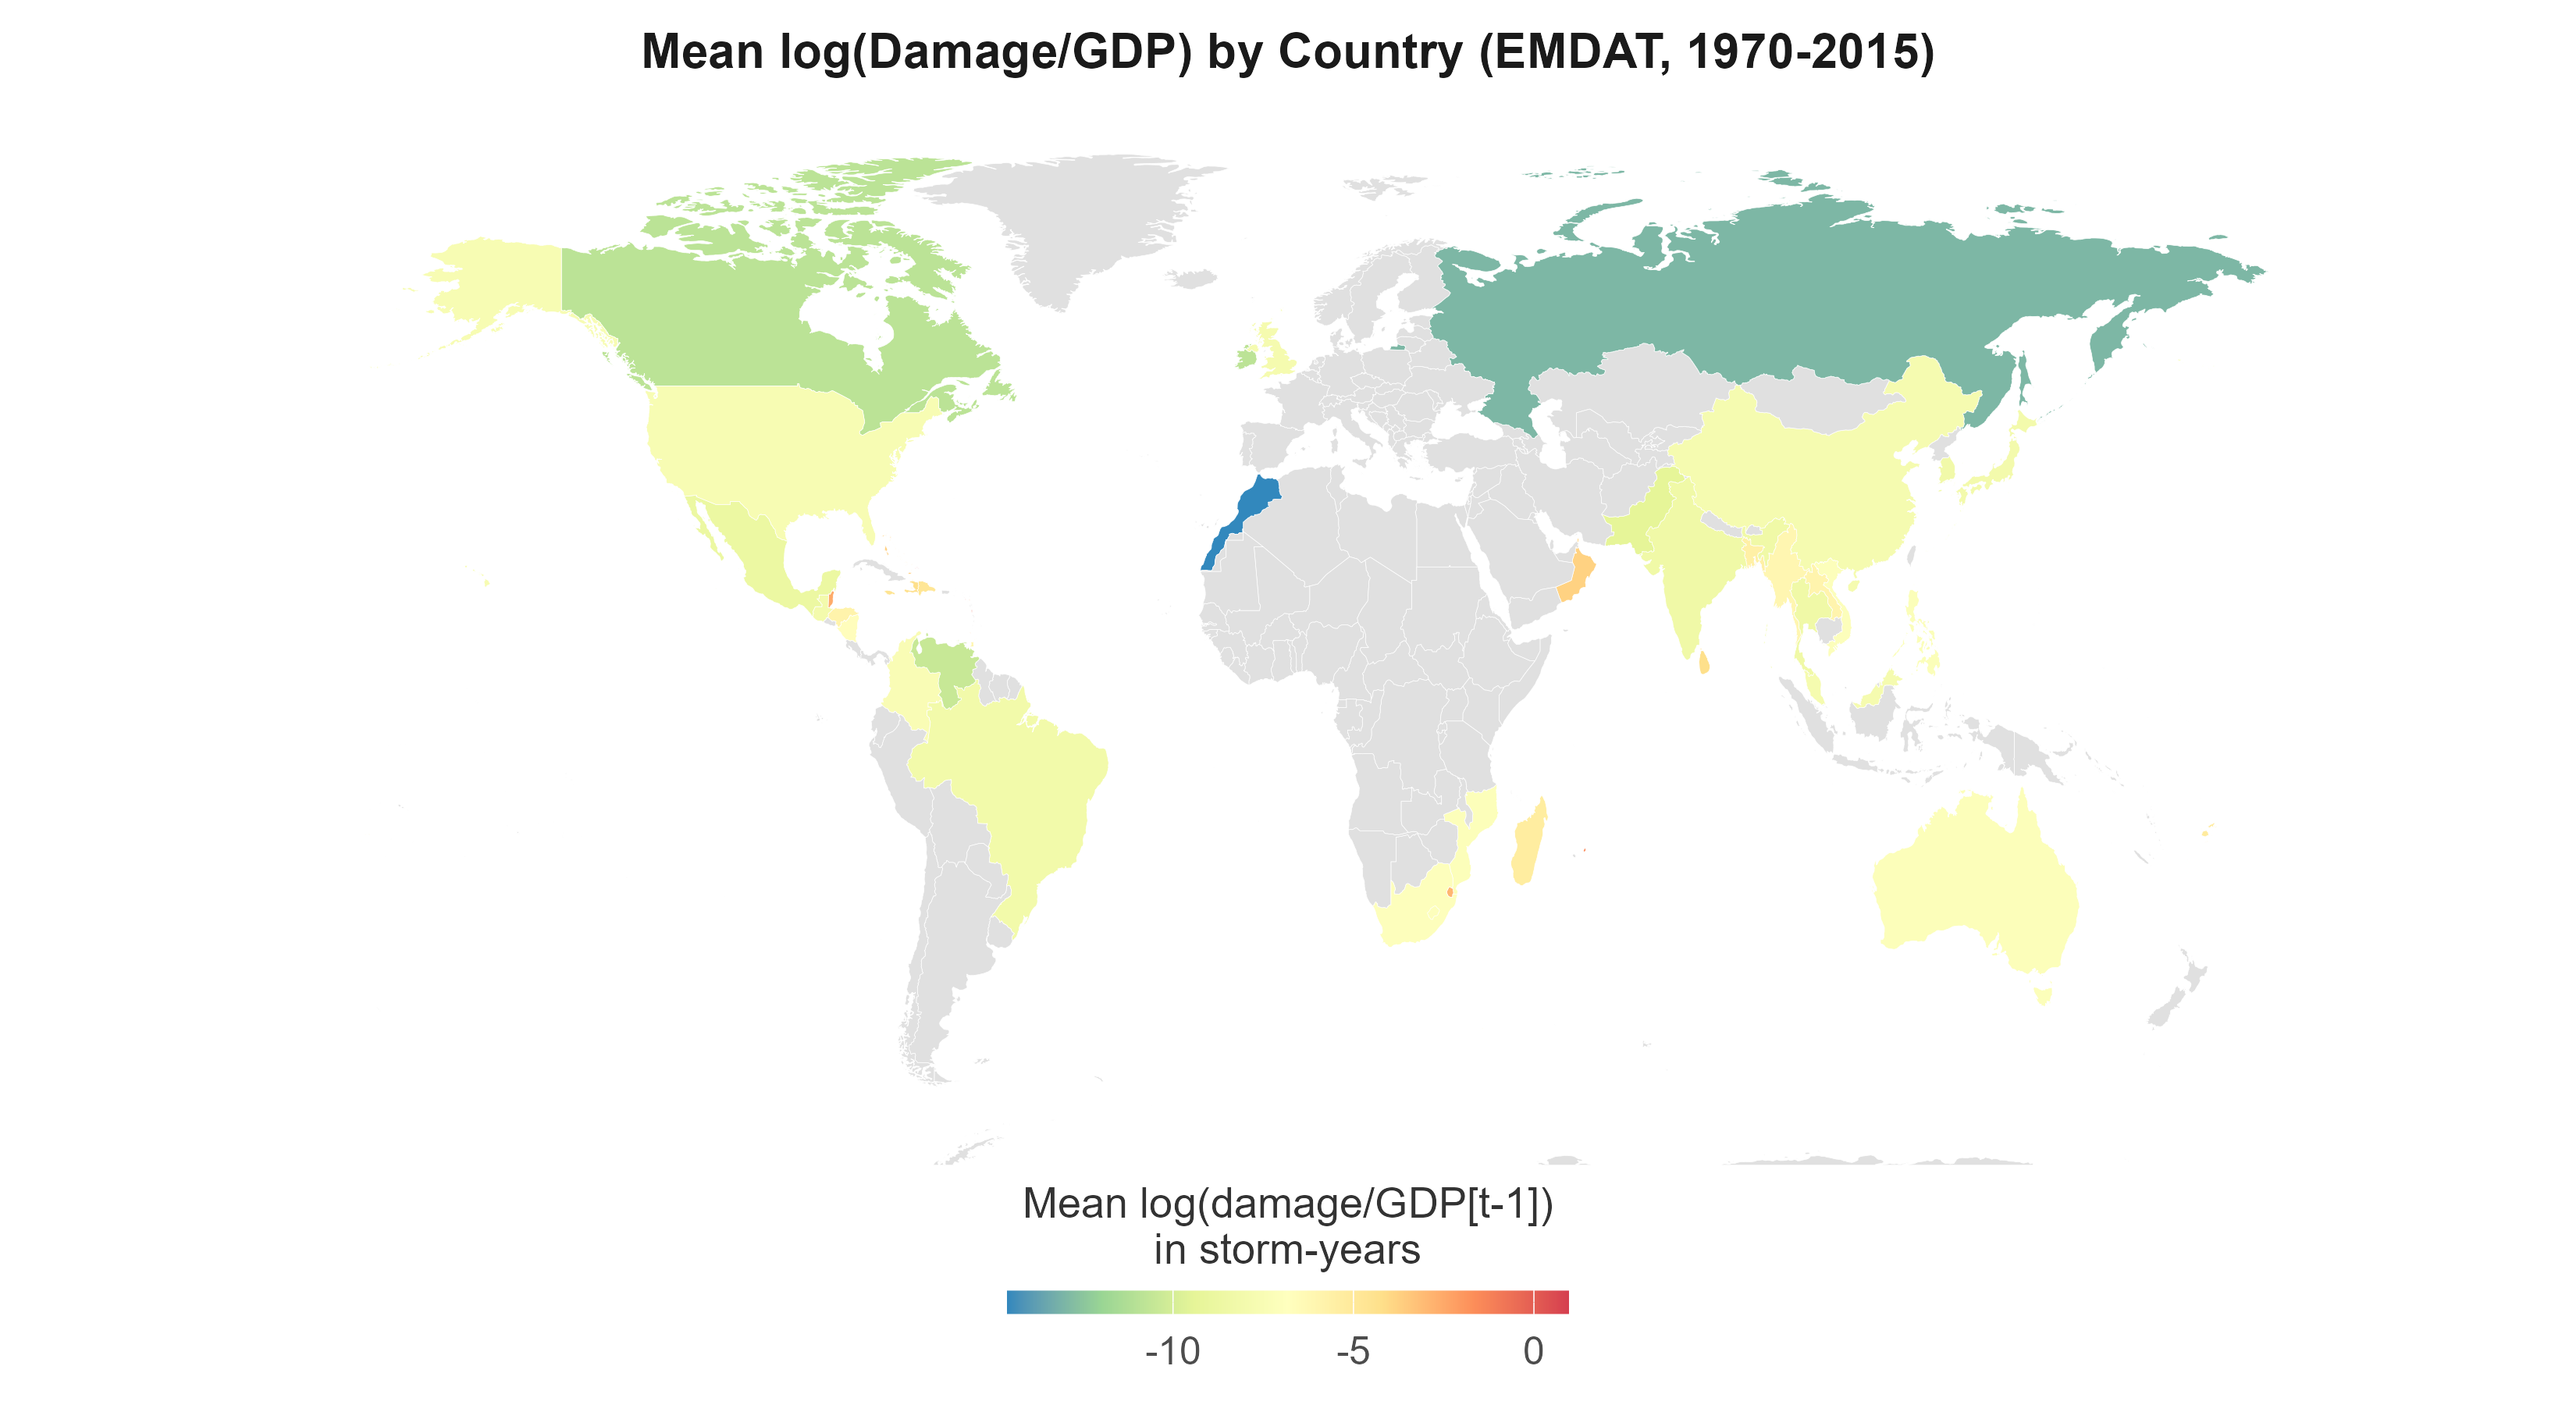
\includegraphics[width=0.92\textwidth,height=0.70\textheight,keepaspectratio]{figures/map_direct_damage.png}

\smallskip\small
Mean $\log(\text{EMDAT damage}/\text{GDP}_{t-1})$ across storm-years by country.
Small island states and South/South-East Asia concentrate the highest
normalised losses; North America and Europe show comparatively low ratios.
\end{frame}

\begin{frame}{Damage Increases with Wind Speed}
\centering
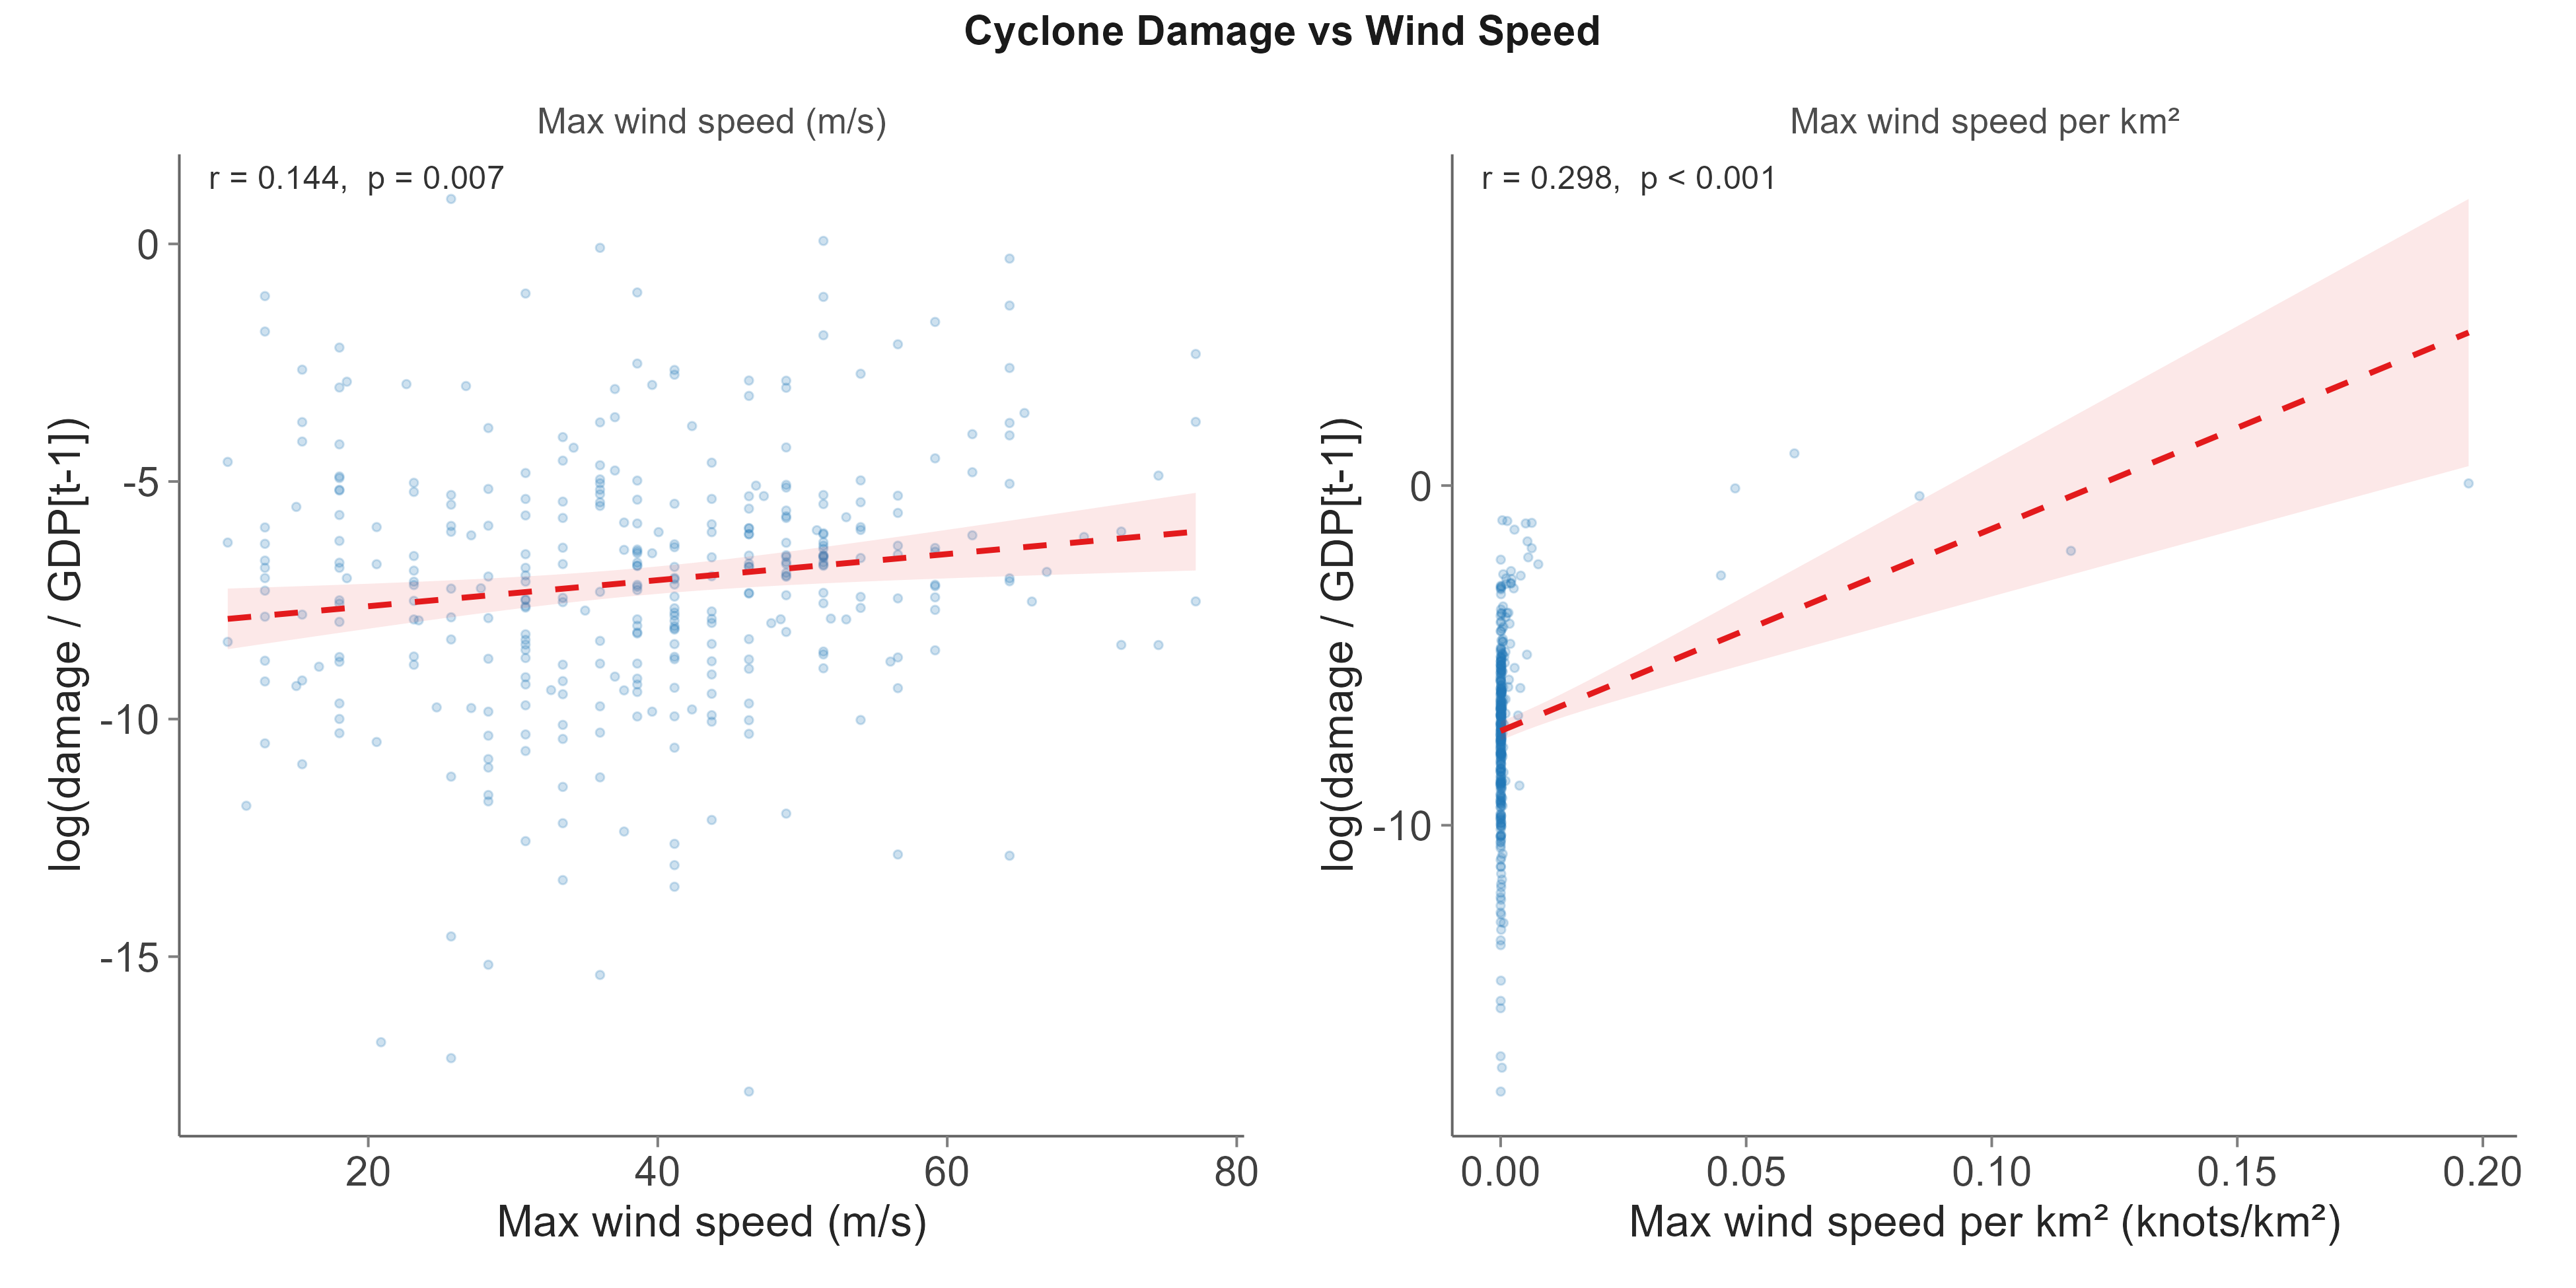
\includegraphics[width=0.92\textwidth,height=0.70\textheight,keepaspectratio]{figures/damage_vs_wind_scatter.png}

\smallskip\small
Left: max wind speed (m/s). Right: max wind per km$^2$ (knots/km$^2$).
Both measures show a significant positive relationship with $\log(\text{damage}/\text{GDP}_{t-1})$.
Pearson $r$ and $p$-value annotated; dashed line is the OLS fit.
\end{frame}

\begin{frame}{Predicted Damage \& Mortality vs Wind Speed}
\centering
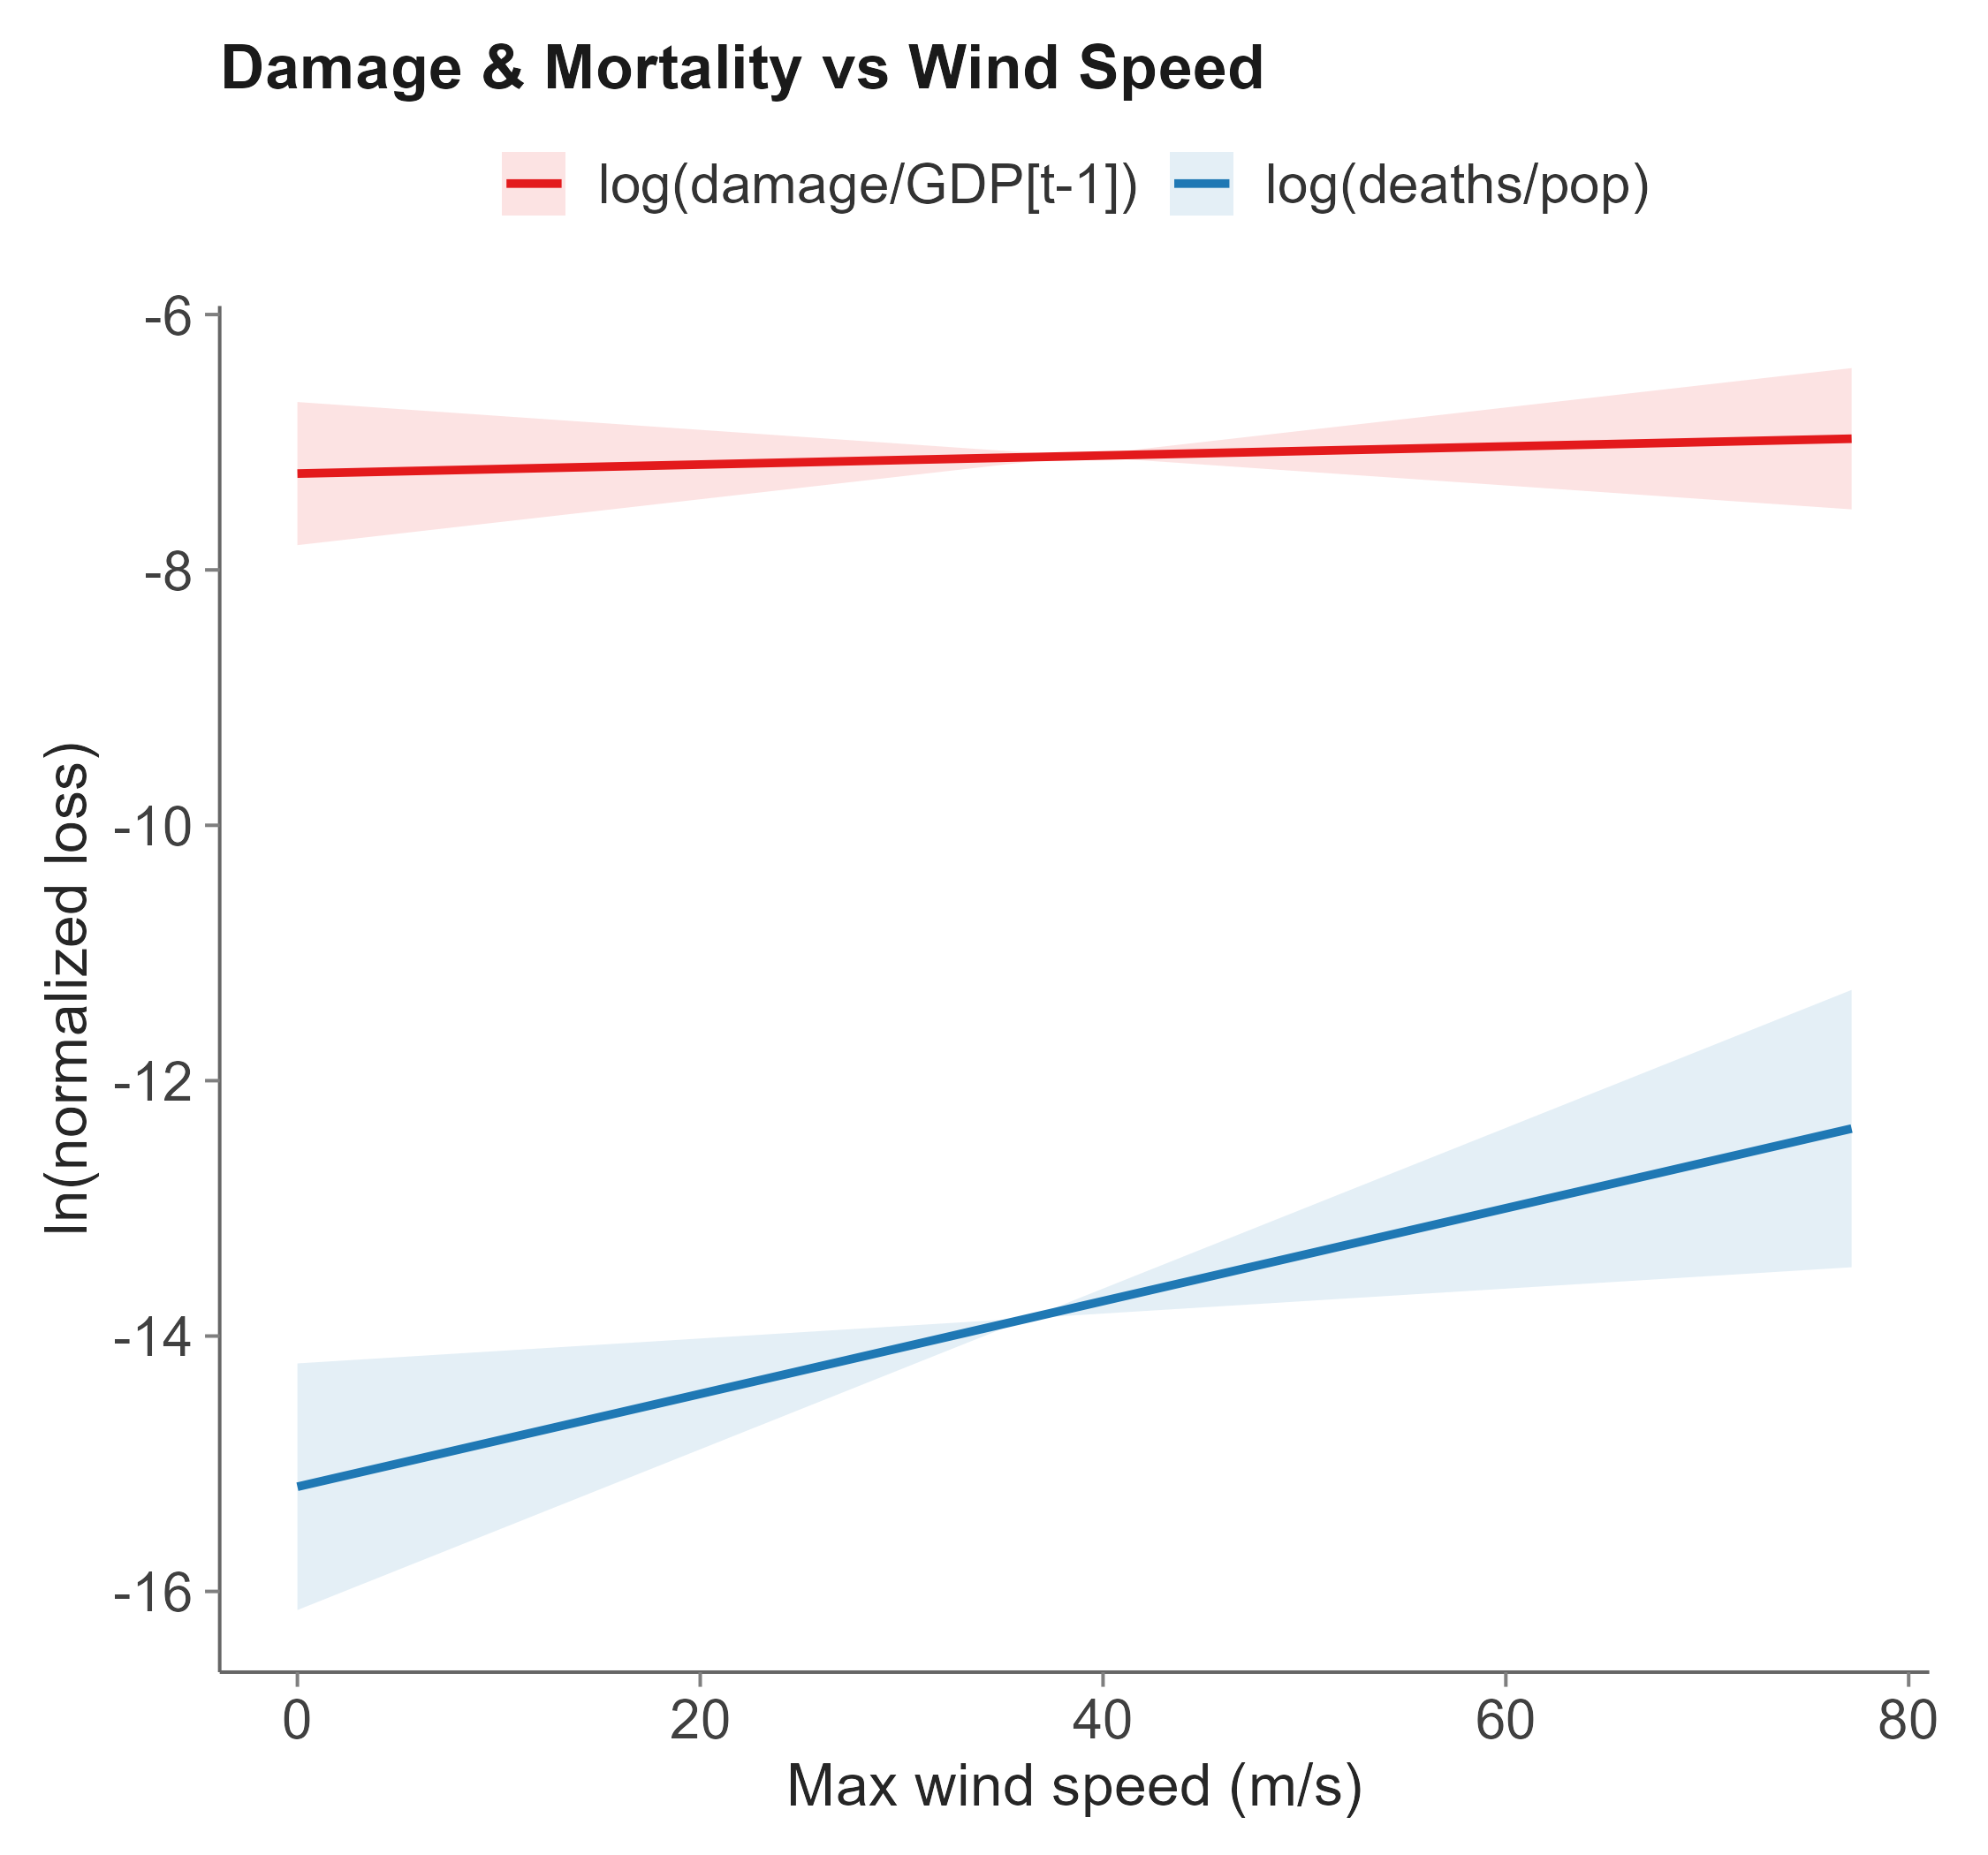
\includegraphics[width=0.82\textwidth,height=0.70\textheight,keepaspectratio]{figures/damage_deaths_vs_maxwind_feols.png}

\smallskip\small
Predicted $\ln(\text{normalised loss})$ as a function of max wind speed,
OLS with country quadratic trends and region$\times$year FE.
Both $\log(\text{damage}/\text{GDP}_{t-1})$ and $\log(\text{deaths/pop})$ rise with wind,
with mortality losses steeper at high intensities.
\end{frame}

\begin{frame}{Category-Specific Damage Coefficients}
\centering
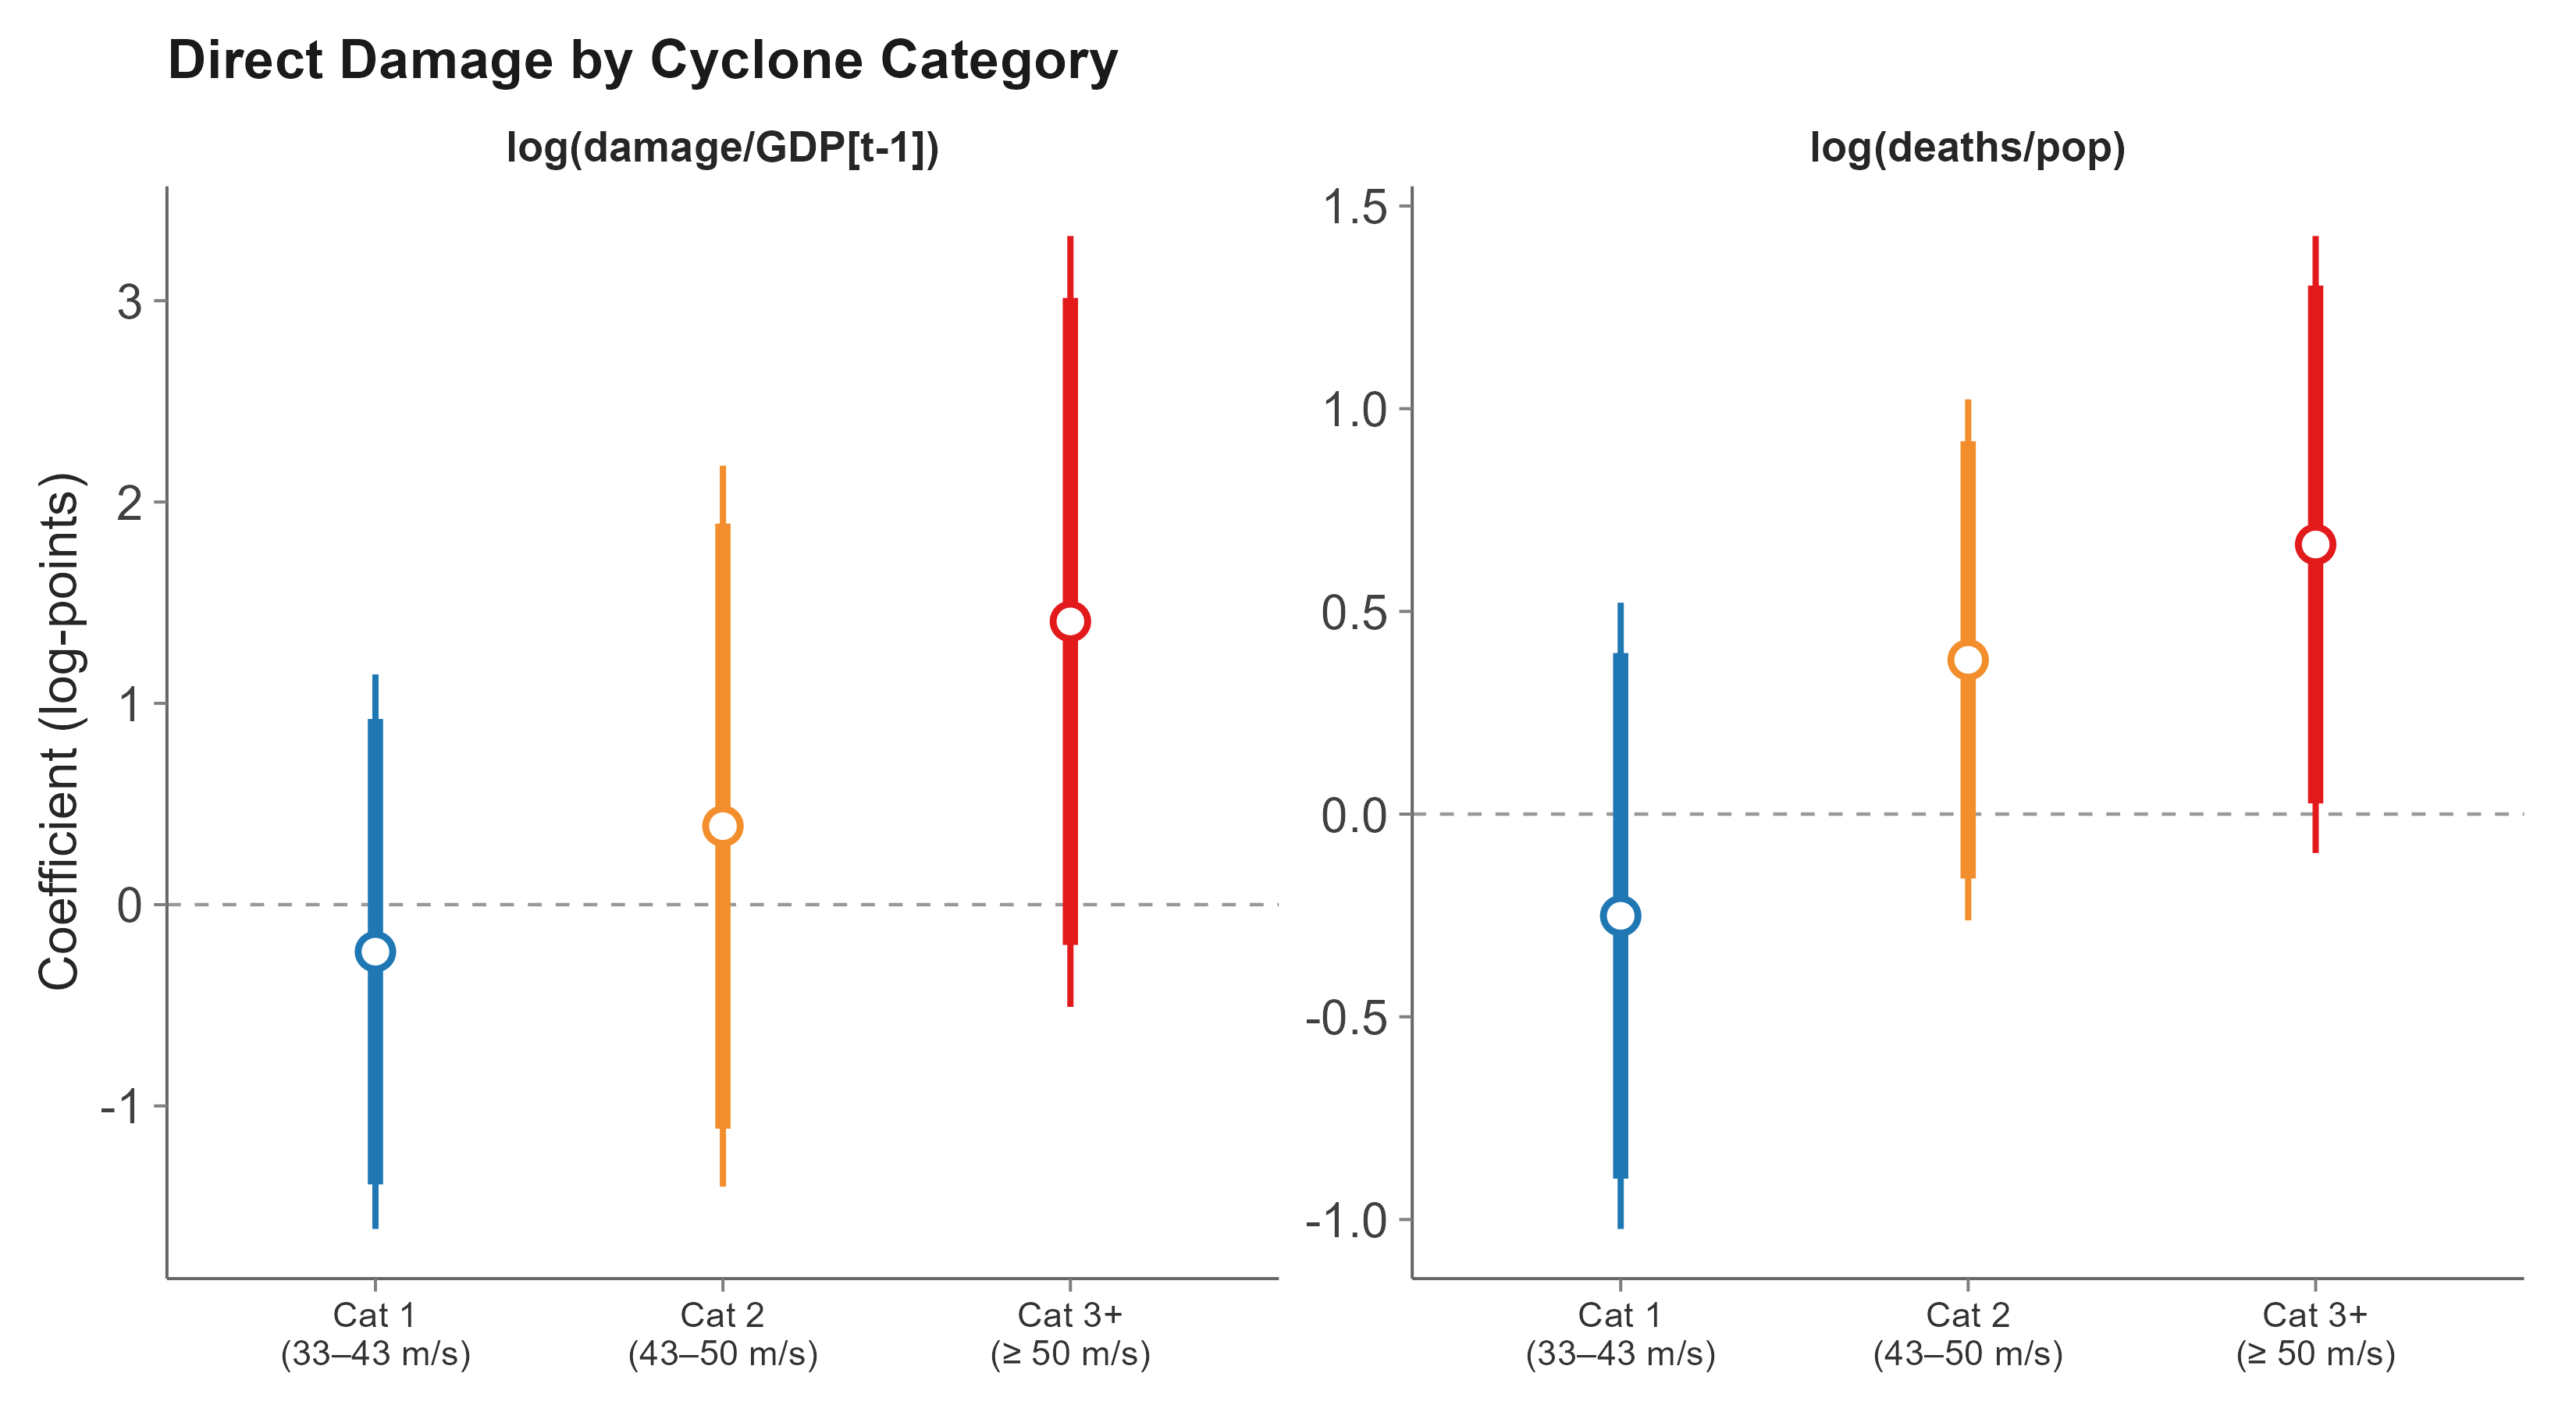
\includegraphics[width=0.92\textwidth,height=0.70\textheight,keepaspectratio]{figures/direct_damage_coef.png}

\smallskip\small
Contemporaneous OLS coefficient (country-clustered SE) on three
\emph{mutually exclusive} category indicators.
Left panel: $\log(\text{damage}/\text{GDP}_{t-1})$; right panel: $\log(\text{deaths/pop})$.
Thick bar = 90\,\% CI; thin bar = 95\,\% CI.
Both damage and mortality rise monotonically with storm intensity.
\end{frame}

% ===============================================================
\section{GDP Growth Response}
% ===============================================================
{\hideframenumber\begin{frame}\sectionpage\end{frame}\showframenumber}

\begin{frame}{GDP LP IRF by Cyclone Intensity}
\centering
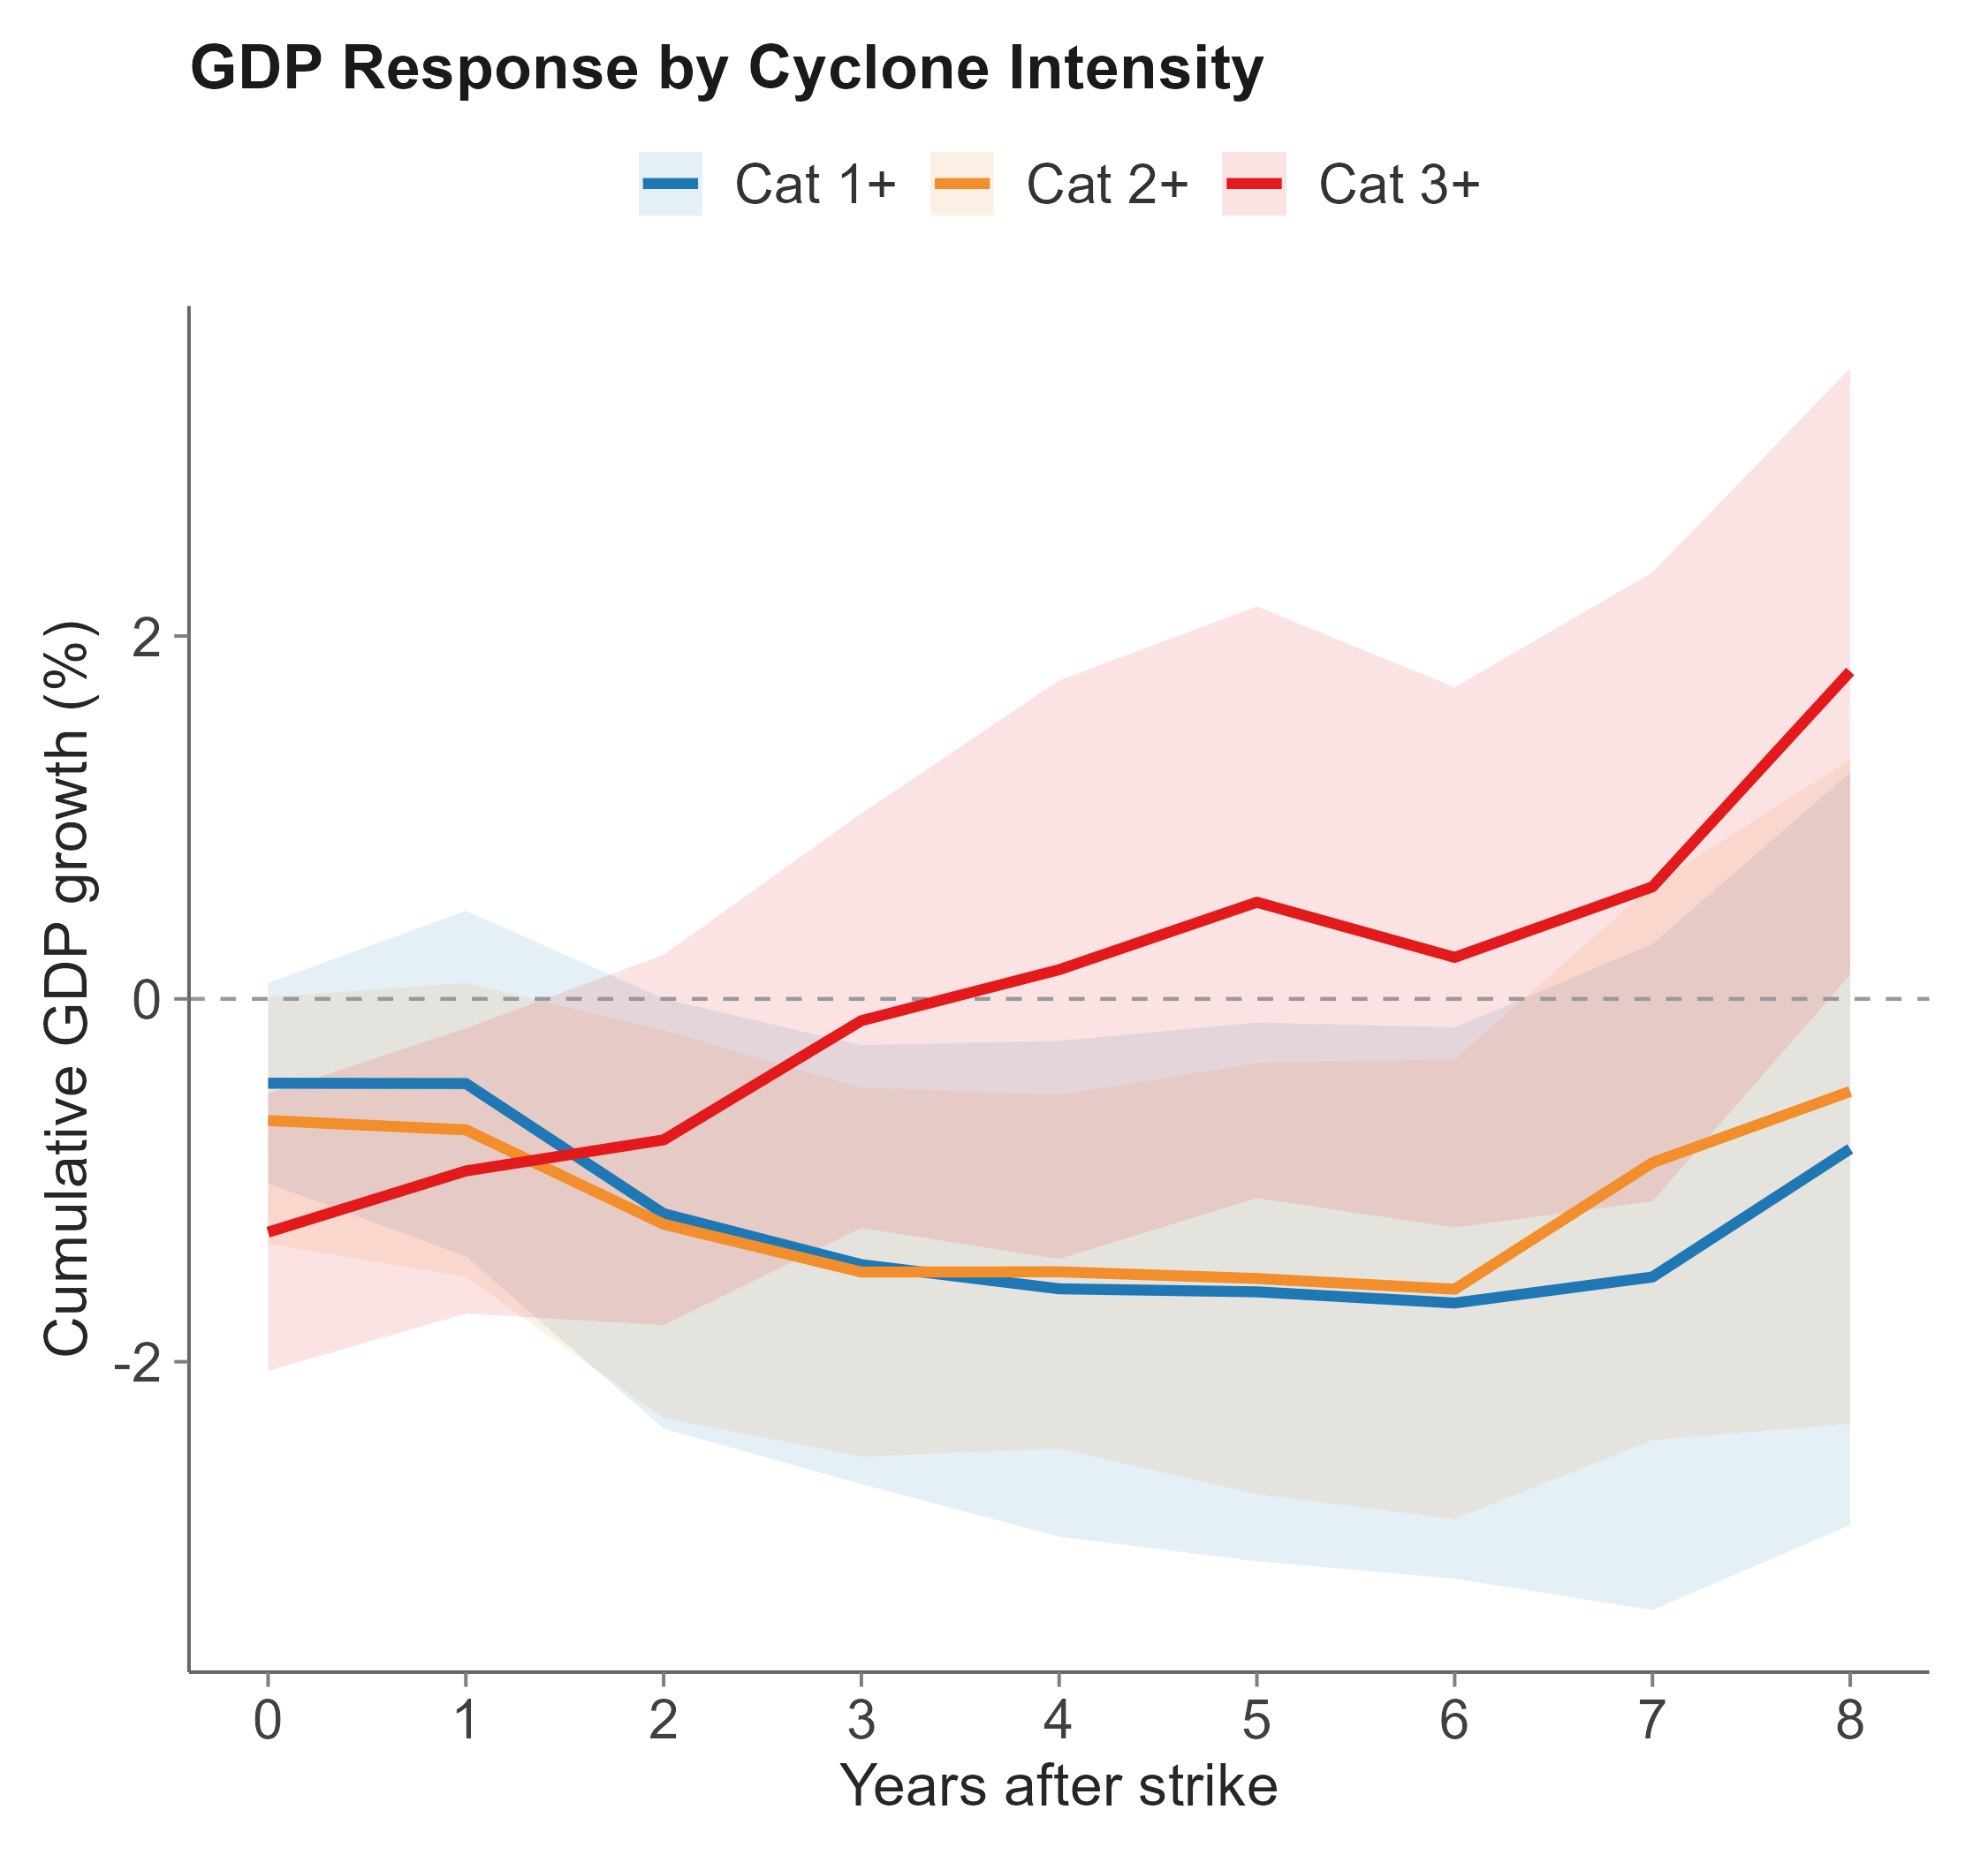
\includegraphics[width=0.82\textwidth,height=0.70\textheight,keepaspectratio]{figures/irf_gdp_by_category.png}

\smallskip\small
LP impulse responses of $\log$ GDP per capita to Cat~1$+$, Cat~2$+$, and
Cat~3$+$ binary shocks. Cat~3$+$ strikes produce the largest and most
persistent growth drag; Cat~1$+$ effects are smaller and recover faster.
Shaded bands: 95\,\% Driscoll--Kraay confidence intervals.
\end{frame}

% ===============================================================
\section{Damage-Conditioned GDP Response}
% ===============================================================
{\hideframenumber\begin{frame}\sectionpage\end{frame}\showframenumber}

\begin{frame}{Does Higher Prior Damage Amplify GDP Losses?}

If direct physical damage \emph{mediates} the wind--GDP transmission:
\begin{itemize}
  \item Countries with larger $\log(\text{damage}/\text{GDP}_{t-1})$ in previous years
        are more vulnerable and should exhibit \textbf{deeper} GDP losses
        from the same cyclone shock
  \item The state-dependent LP isolates this channel, holding wind intensity
        (Cat~1$+$ indicator) constant
\end{itemize}

\medskip
\textbf{Specification:}
\[
  \Delta_h\log y_{it}
  = \underbrace{\beta_h + \gamma_h\,\log\!\left(\frac{\text{damage}_{it}}{\text{GDP}_{it}}\right)}_{\text{ME}(D_{it}=1)}
  \times \mathbf{1}[\text{Cat\,1}+]_{it} + \cdots
\]
Marginal effect evaluated at $p_{25}$ and $p_{75}$ of
contemporaneous $\log(\text{damage}/\text{GDP}_{t-1})$ via delta method.
\end{frame}

\begin{frame}{State-Dependent LP: GDP Response Conditional on Damage Level}
\centering
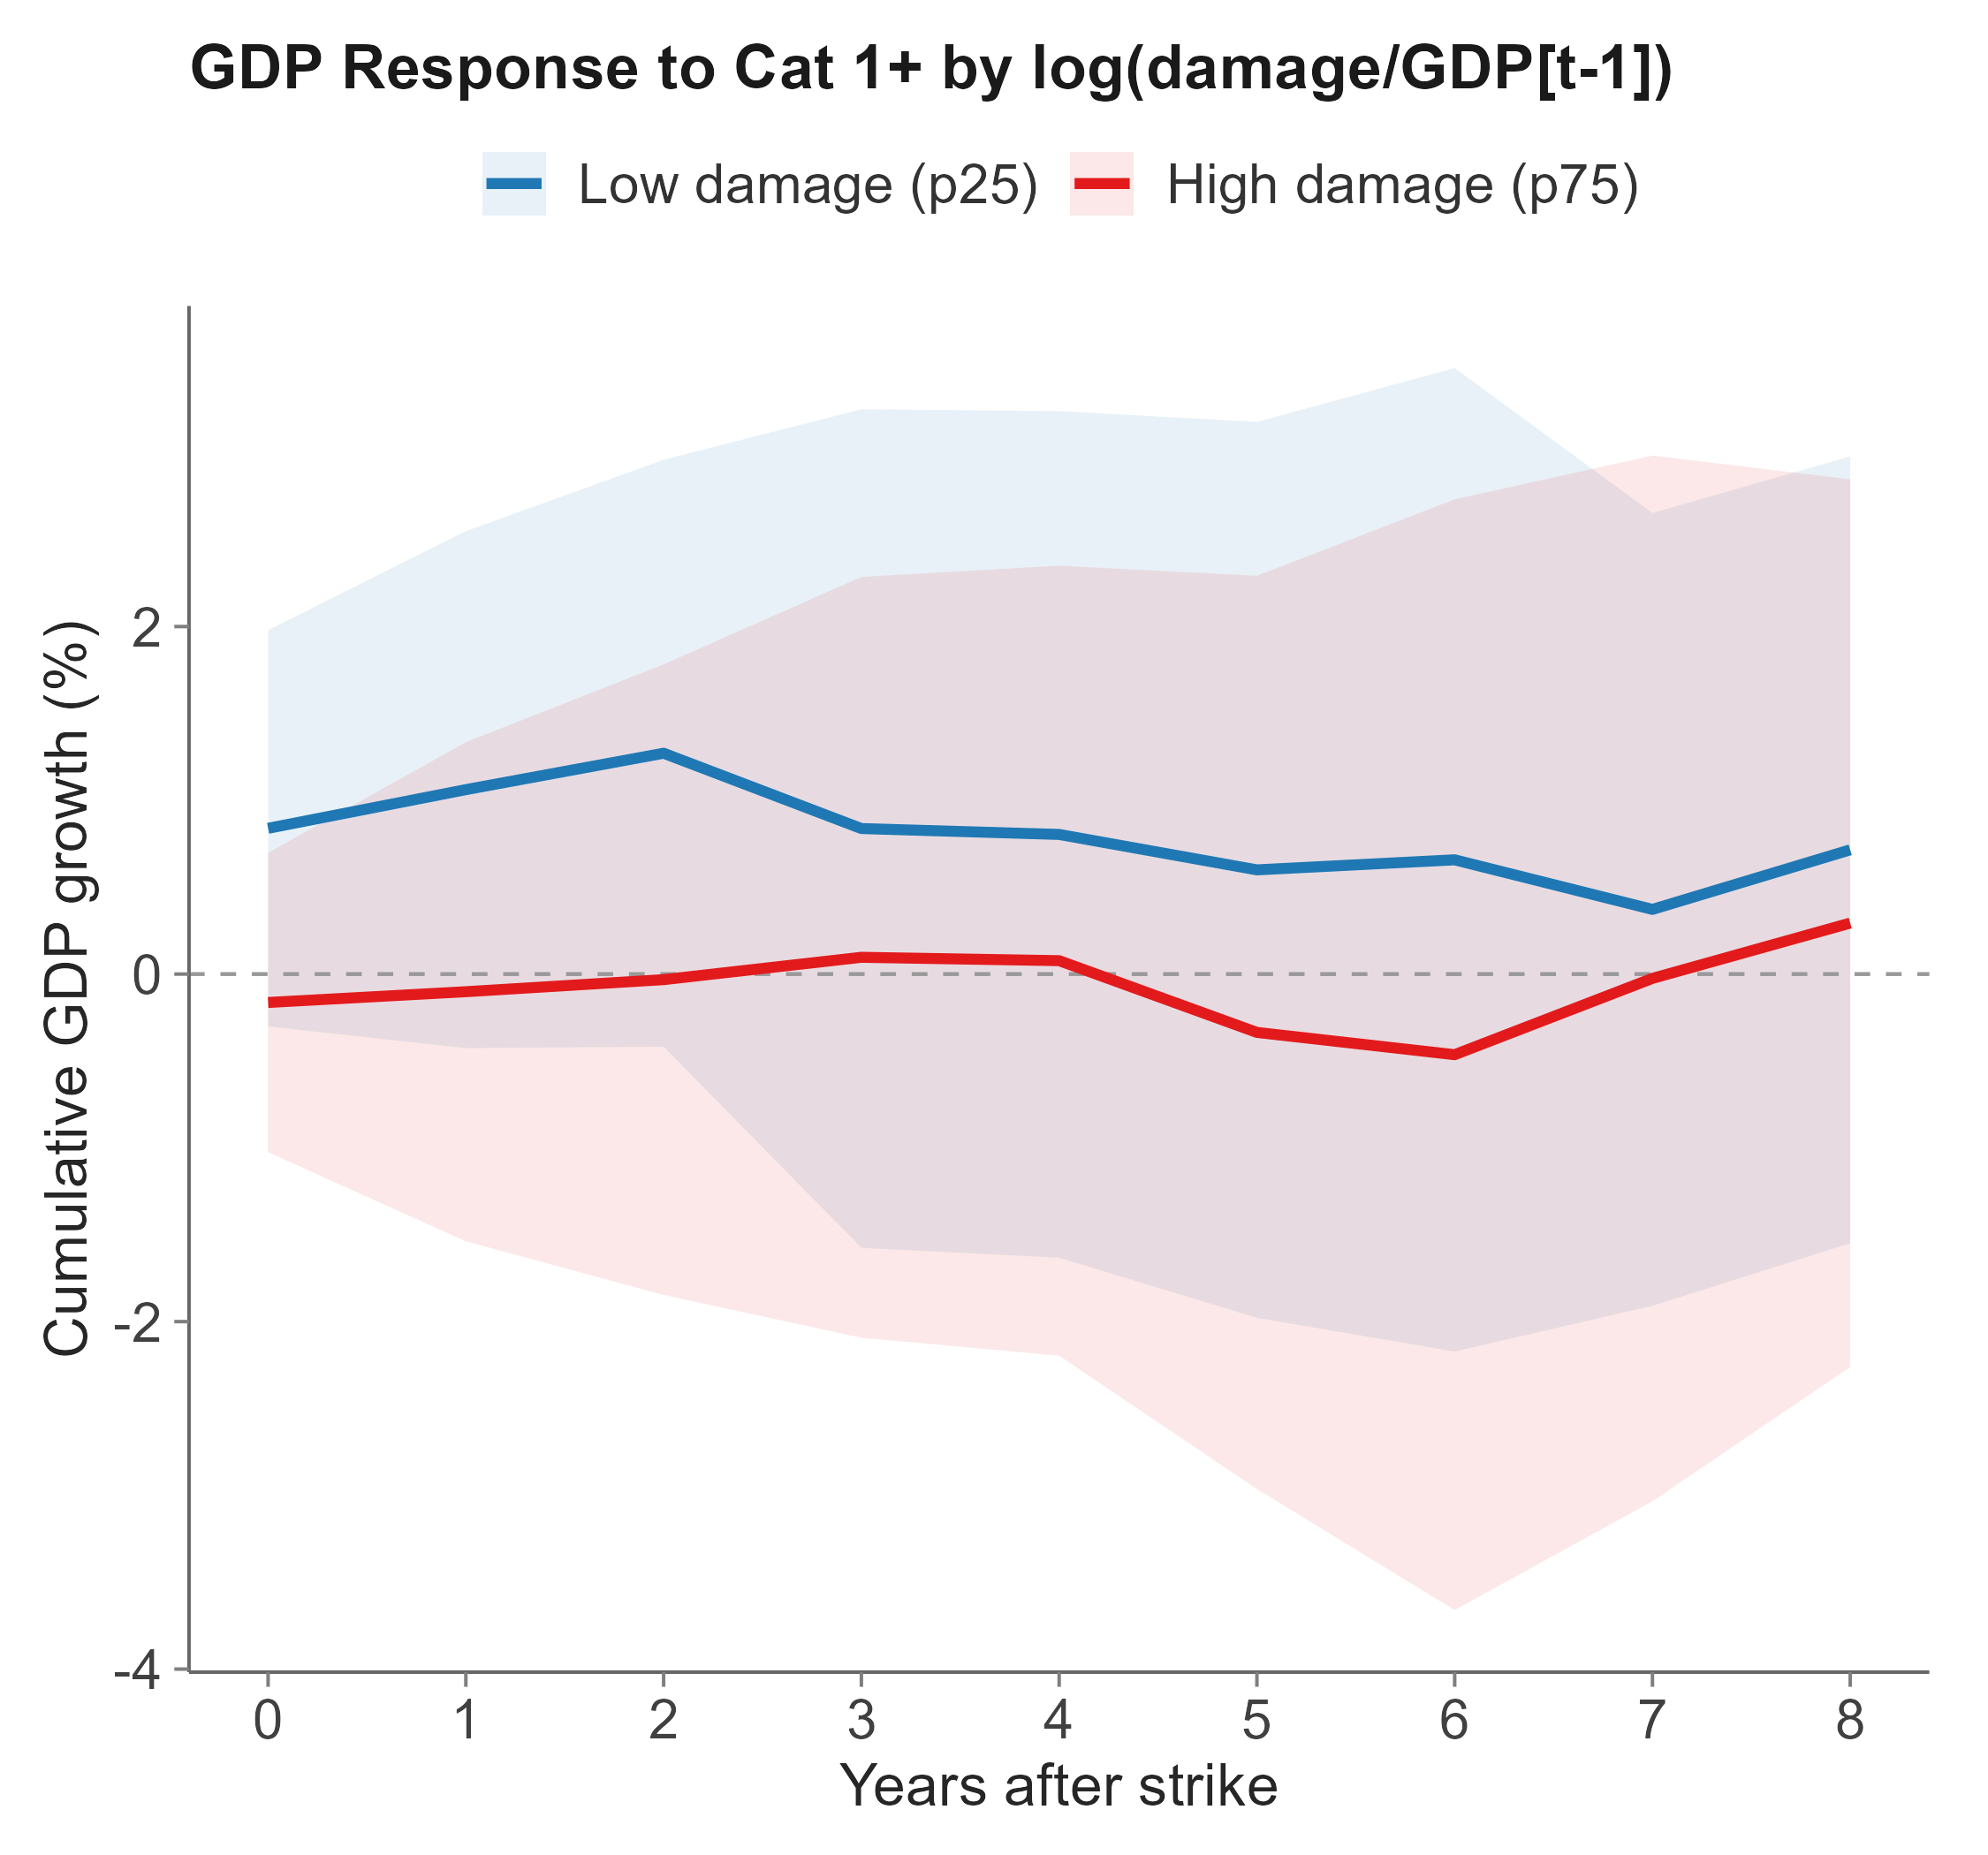
\includegraphics[width=0.82\textwidth,height=0.70\textheight,keepaspectratio]{figures/irf_gdp_state_dep_damage.png}

\smallskip\small
Countries at the \textbf{75th percentile} of prior $\log(\text{damage}/\text{GDP}_{t-1})$
suffer larger and more persistent GDP losses from a Cat~1$+$ strike.
Countries at the \textbf{25th percentile} show a muted response.
Evaluation at p25/p75 matches the binary vulnerability split used in the sub-sample LP.
\end{frame}

\begin{frame}{Sub-Sample LP: GDP IRF by Damage-Vulnerability (Binary)}
\centering
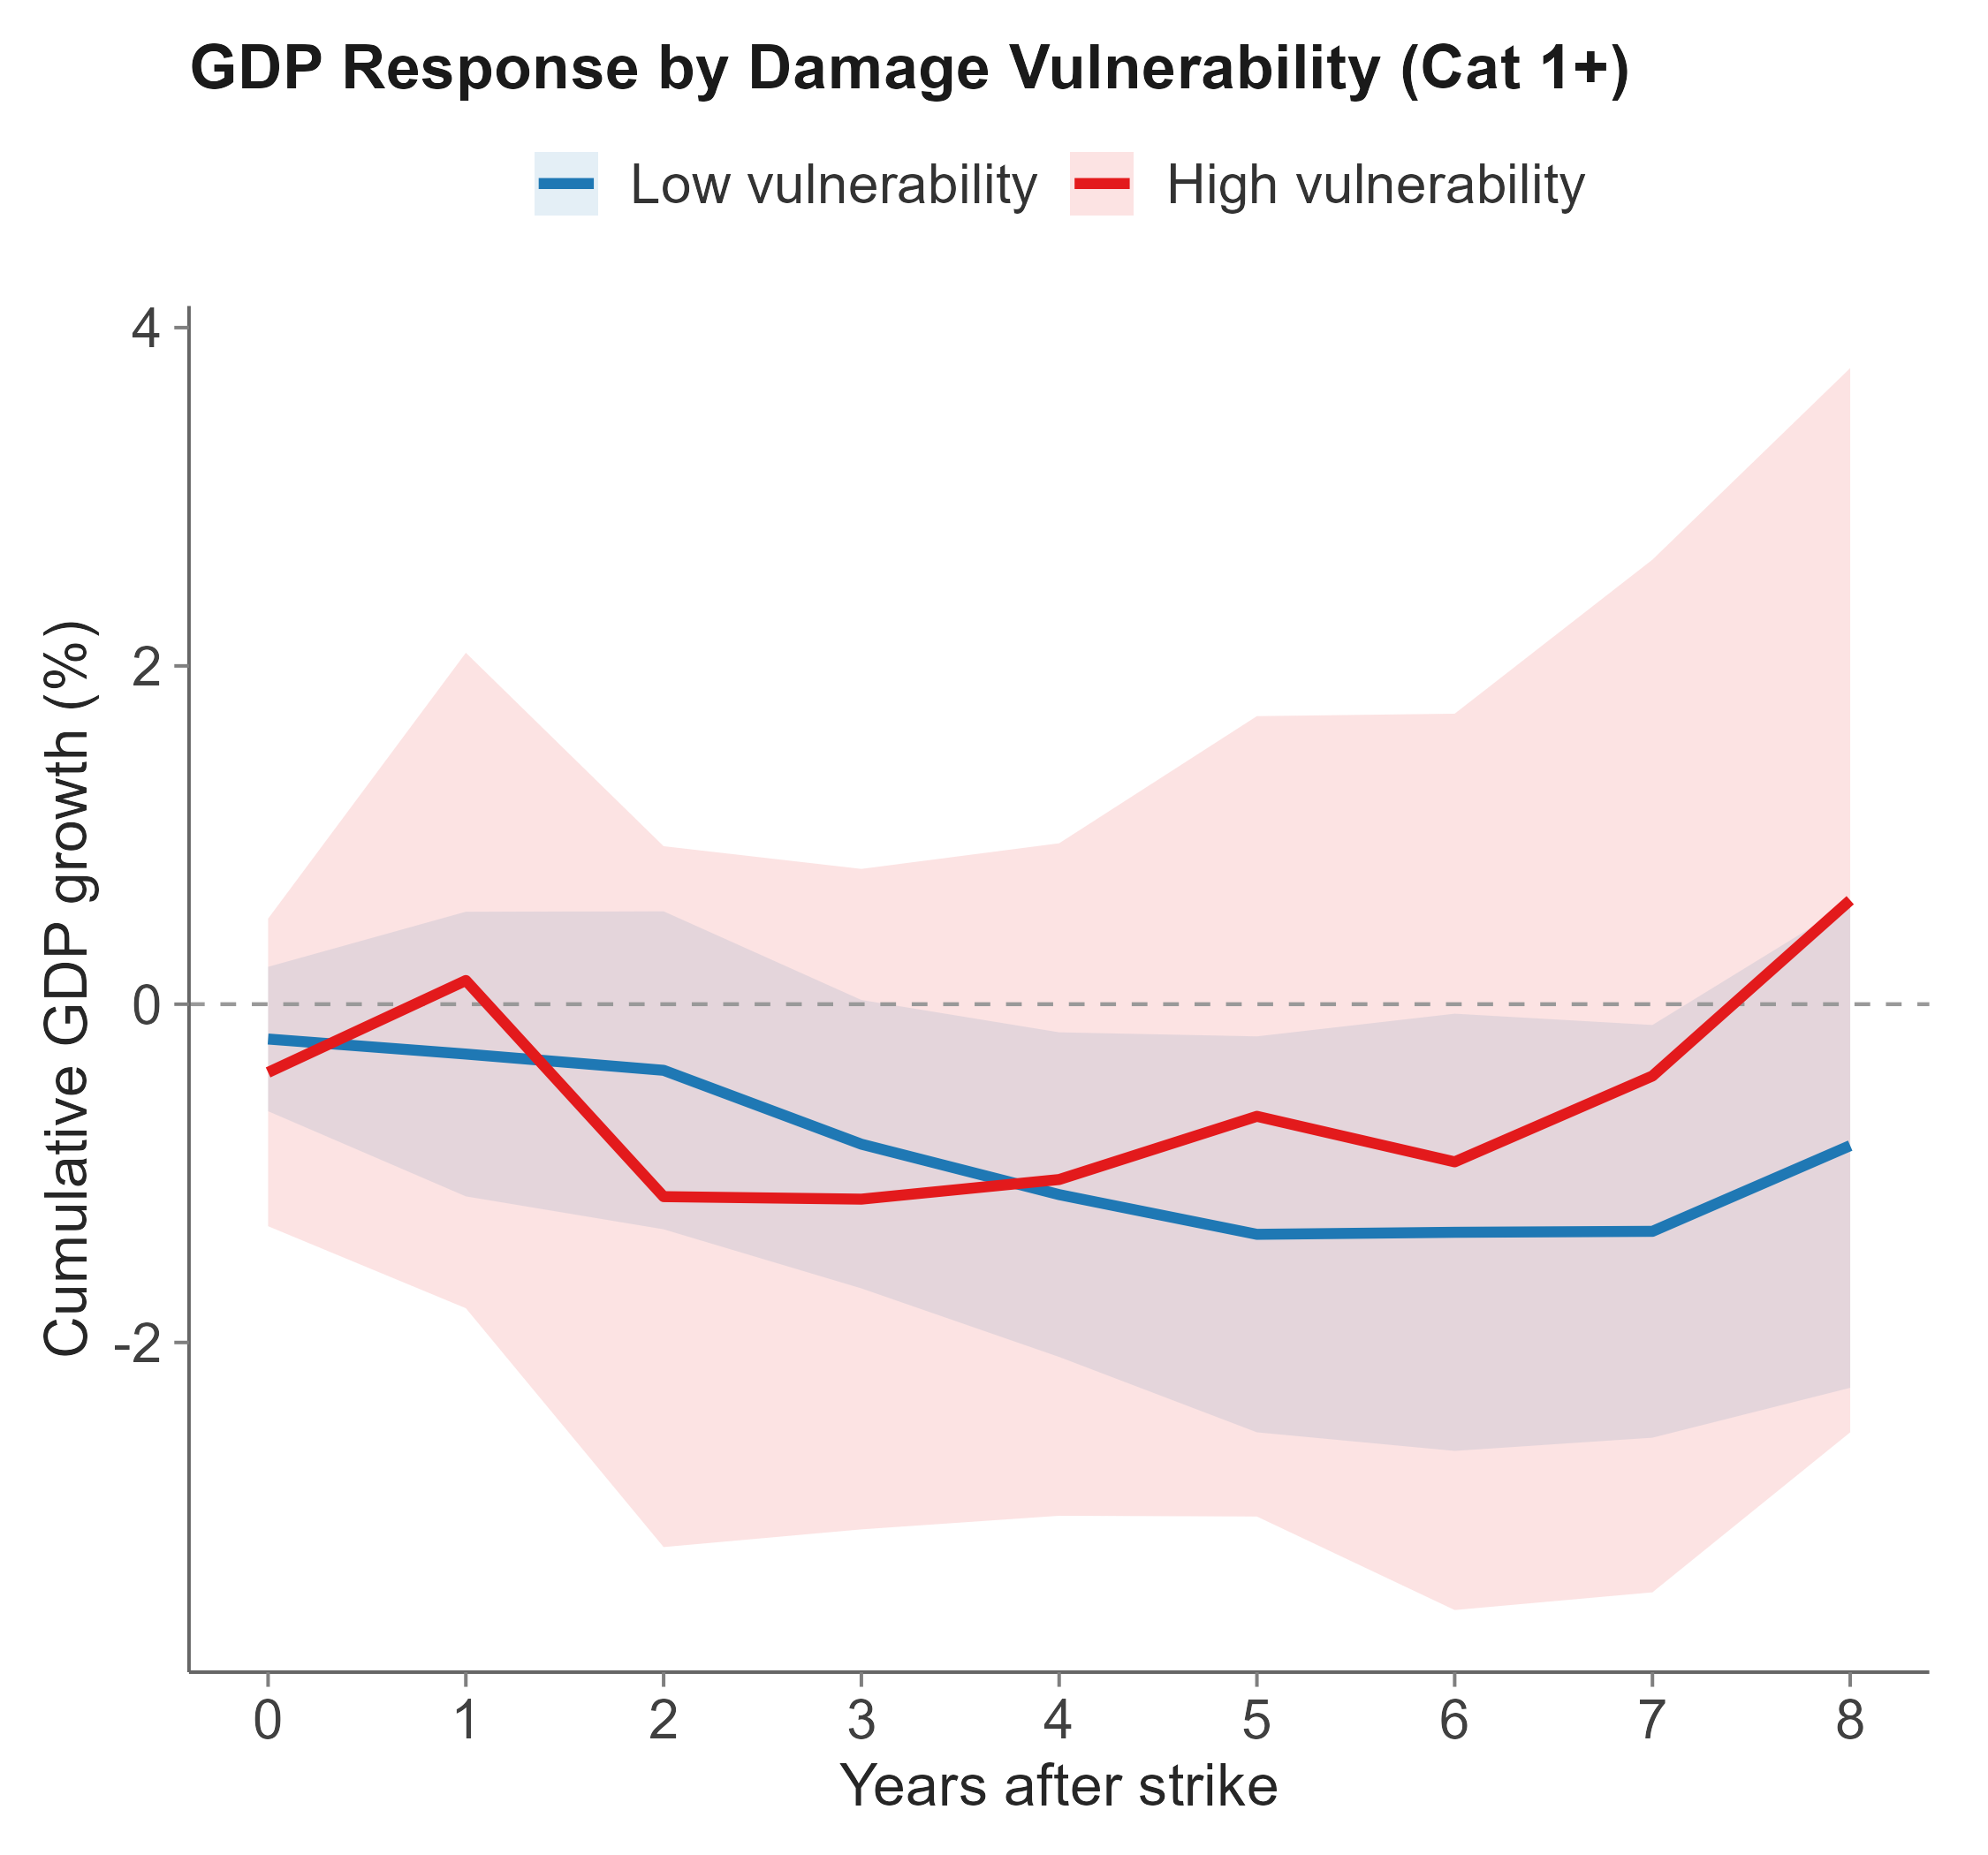
\includegraphics[width=0.82\textwidth,height=0.70\textheight,keepaspectratio]{figures/irf_gdp_by_damage_vuln.png}

\smallskip\small
\textbf{Vulnerability index:} country-mean of $\log(\text{damage}_{t}/\text{GDP}_{t-1})$
in storm-years with positive EMDAT damage.
Countries split at the median into Low and High vulnerability; LP estimated
separately within each sub-sample (all country-years).
\textbf{High-vulnerability} countries show larger GDP losses,
corroborating the state-dependent result with a fully separate estimation sample.
\end{frame}

% ===============================================================
\section{Reconciling the Two Approaches}
% ===============================================================
{\hideframenumber\begin{frame}\sectionpage\end{frame}\showframenumber}

\begin{frame}{Why Do the Two Approaches Differ?}

Both approaches test damage heterogeneity but differ in design:

\medskip
\begin{tabular}{lll}
\toprule
 & \textbf{State-dep LP} & \textbf{Binary sub-sample} \\
\midrule
Variation & Within-country & Between-country \\
State var & Contemporaneous $D_t$ & Long-run mean $\bar{D}_i$ \\
Sample & Damage-positive obs & All country-years \\
Functional form & Linear at p25/p75 & Discrete binary split \\
\bottomrule
\end{tabular}

\medskip
\textbf{Three hypotheses:}
\begin{description}
  \item[H1 Baseline comparison] Full-panel interaction LP (\texttt{lp\_panel\_inter}) as the discrete counterpart to the continuous state-dep LP.
  \item[H2 Within vs.\ between] State-dep exploits annual fluctuations in damage;
        binary split exploits permanent country differences.
  \item[H3 Functional form] Linear interaction at p25/p75 vs.\ discrete binary split.
\end{description}
\end{frame}

\begin{frame}{EDA: Contemporaneous Damage by Vulnerability Group}
\centering
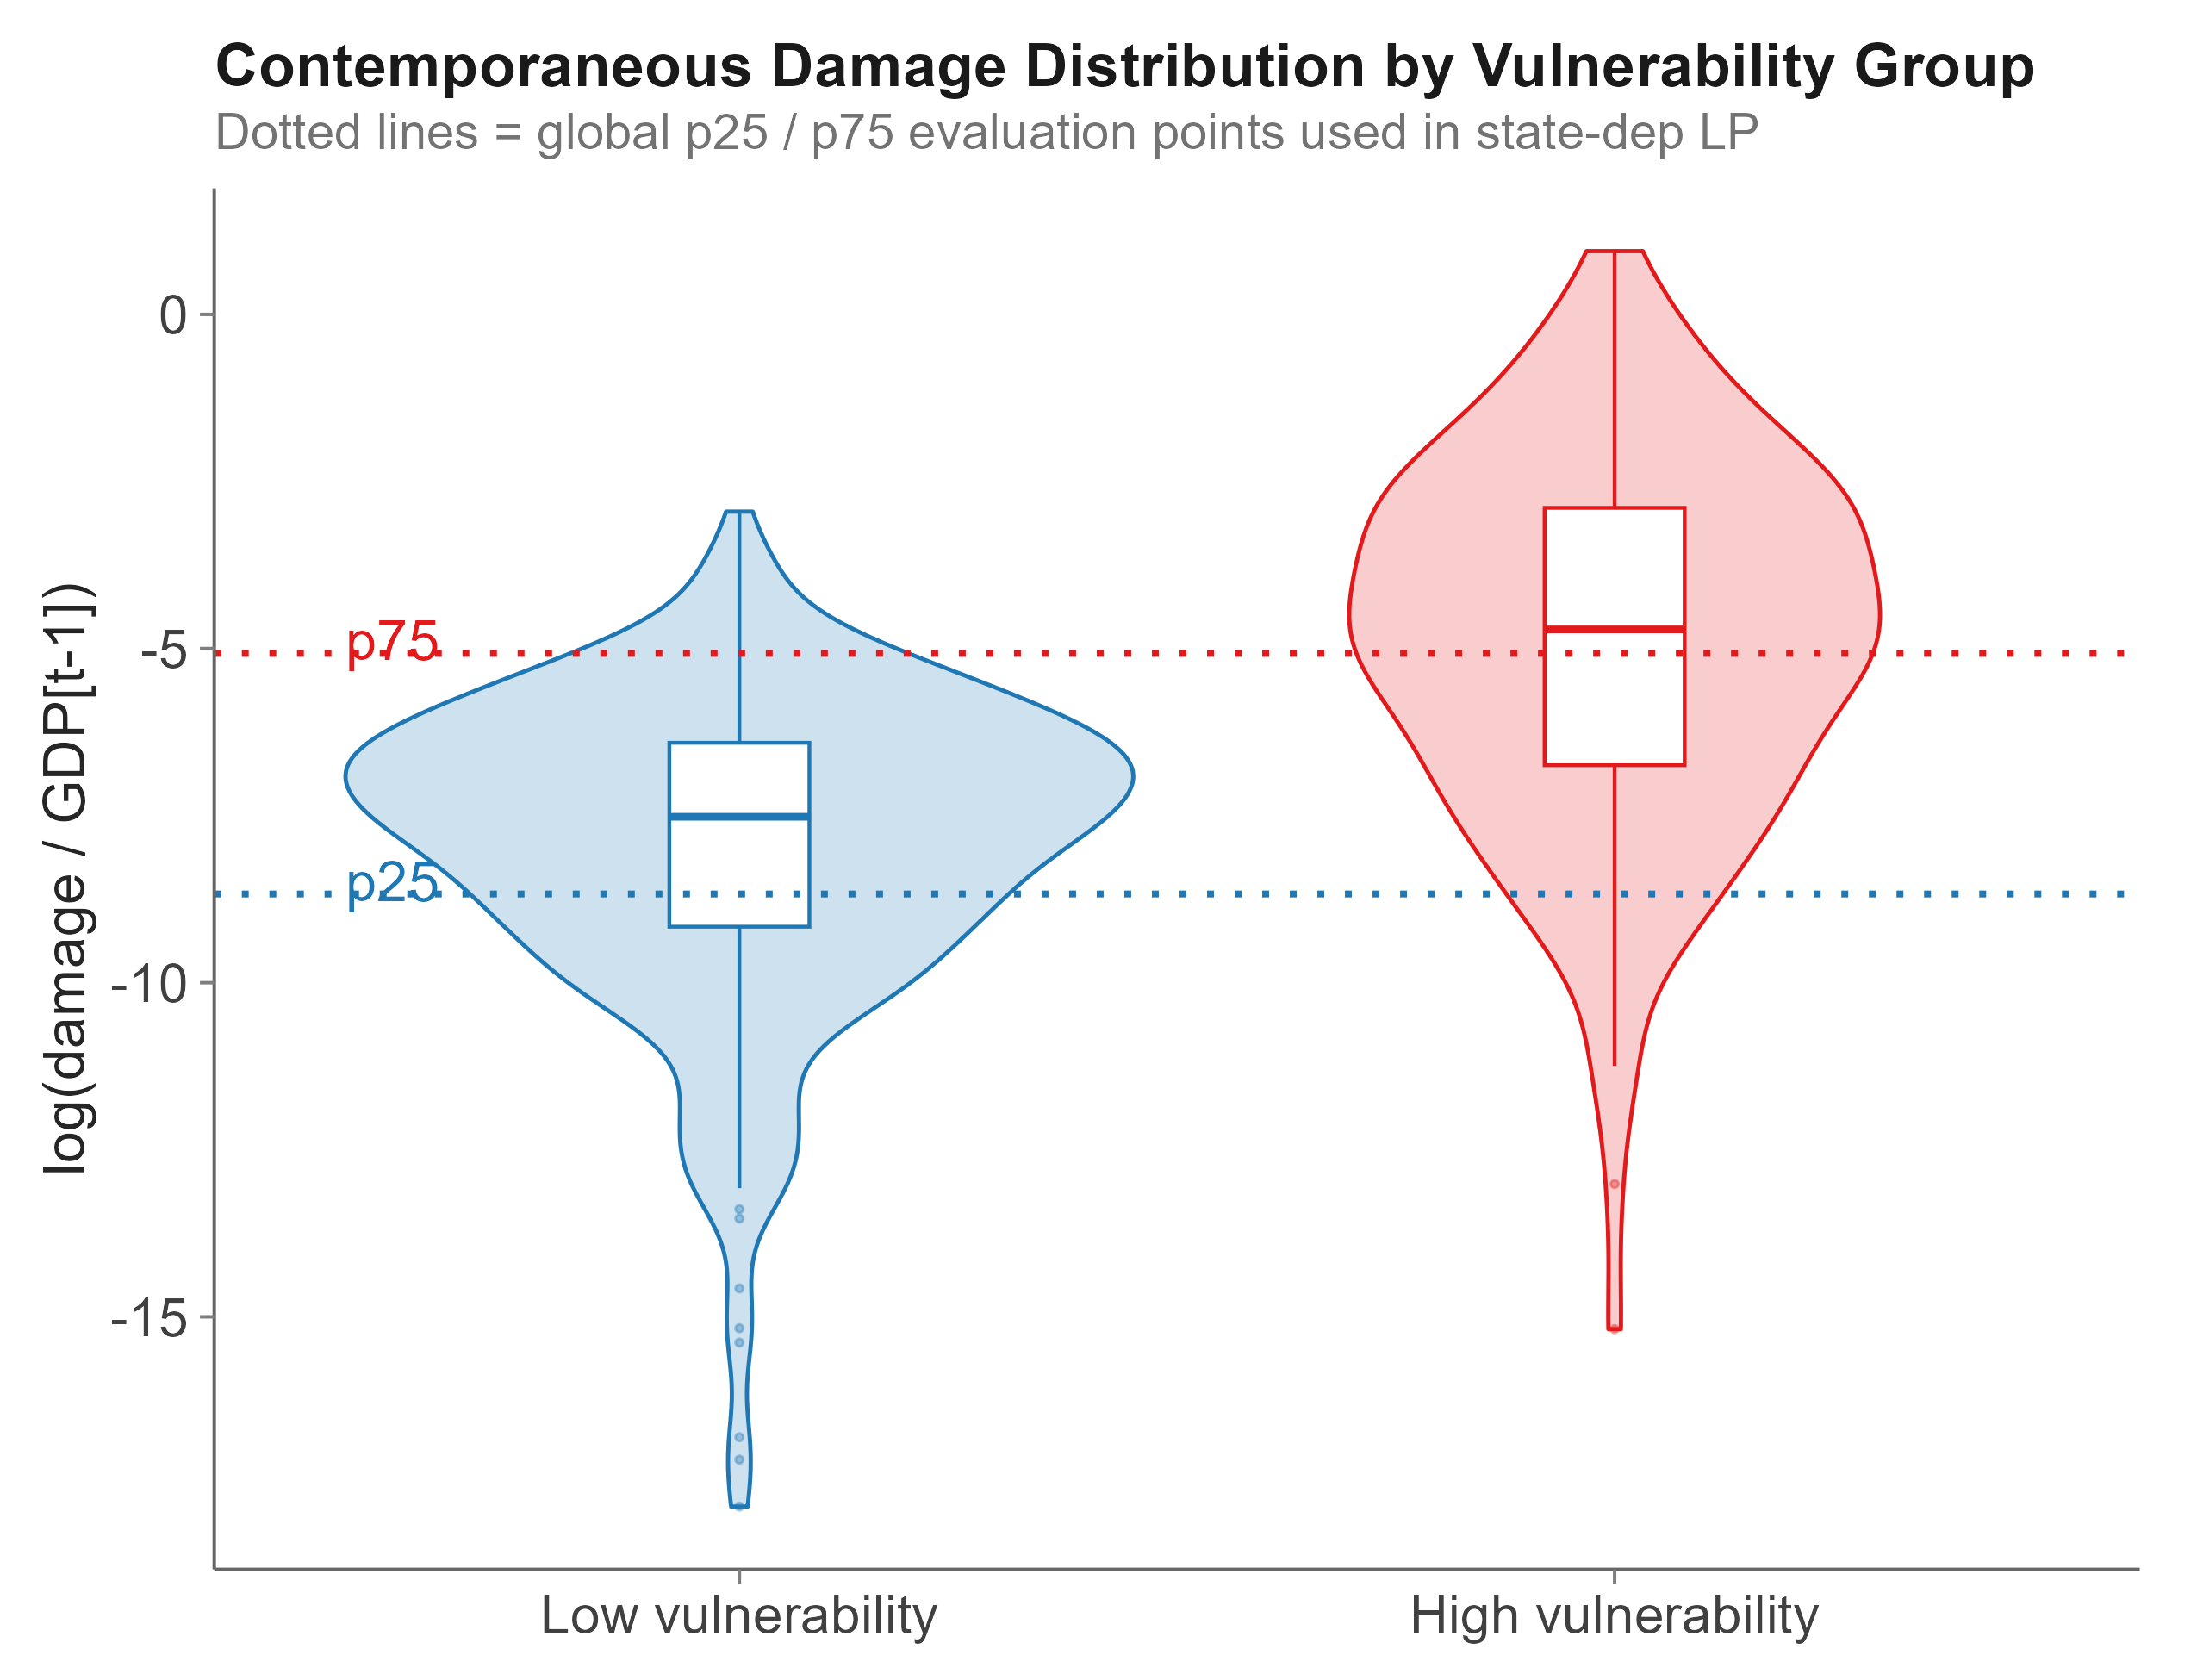
\includegraphics[width=0.88\textwidth,height=0.70\textheight,keepaspectratio]{figures/reconcile_damage_dist.png}

\smallskip\small
Distribution of contemporaneous $\log(\text{damage}/\text{GDP}_{t-1})$ in
storm-years with positive damage, by binary vulnerability group.
Dotted lines mark the global p25/p75 evaluation points used in the state-dep LP.
Overlap between groups indicates that the permanent vulnerability index and
the contemporaneous state variable are measuring related but distinct objects.
\end{frame}

\begin{frame}{Vulnerability Index Construction}

\textbf{Definition:} for each country $i$, compute the mean of
$\log(\text{damage}_{it}/\text{GDP}_{i,t-1})$ over all storm-years with
positive EMDAT damage:
\[
  v_i = \frac{1}{|S_i|}\sum_{t \in S_i}
        \log\!\left(\frac{\text{damage}_{it}}{\text{GDP}_{i,t-1}}\right),
  \quad S_i = \{t : \text{maxwind}_{it}>0,\; \text{damage}_{it}>0\}
\]
Countries are then split at the median of $v_i$ into Low and High vulnerability.
Countries with no positive-damage storm record receive no assignment (NA).

\medskip
\textbf{Why the log?}
\begin{itemize}
  \item Consistent with the state-dep LP state variable
        ($\log D_t/\text{GDP}_{t-1}$)
  \item Compresses extreme values; damage/GDP is heavily right-skewed
  \item Ensures the vulnerability index lives on the same scale as the
        interaction term
\end{itemize}
\end{frame}

\begin{frame}{Map: Vulnerability Binary Split by Country}
\centering
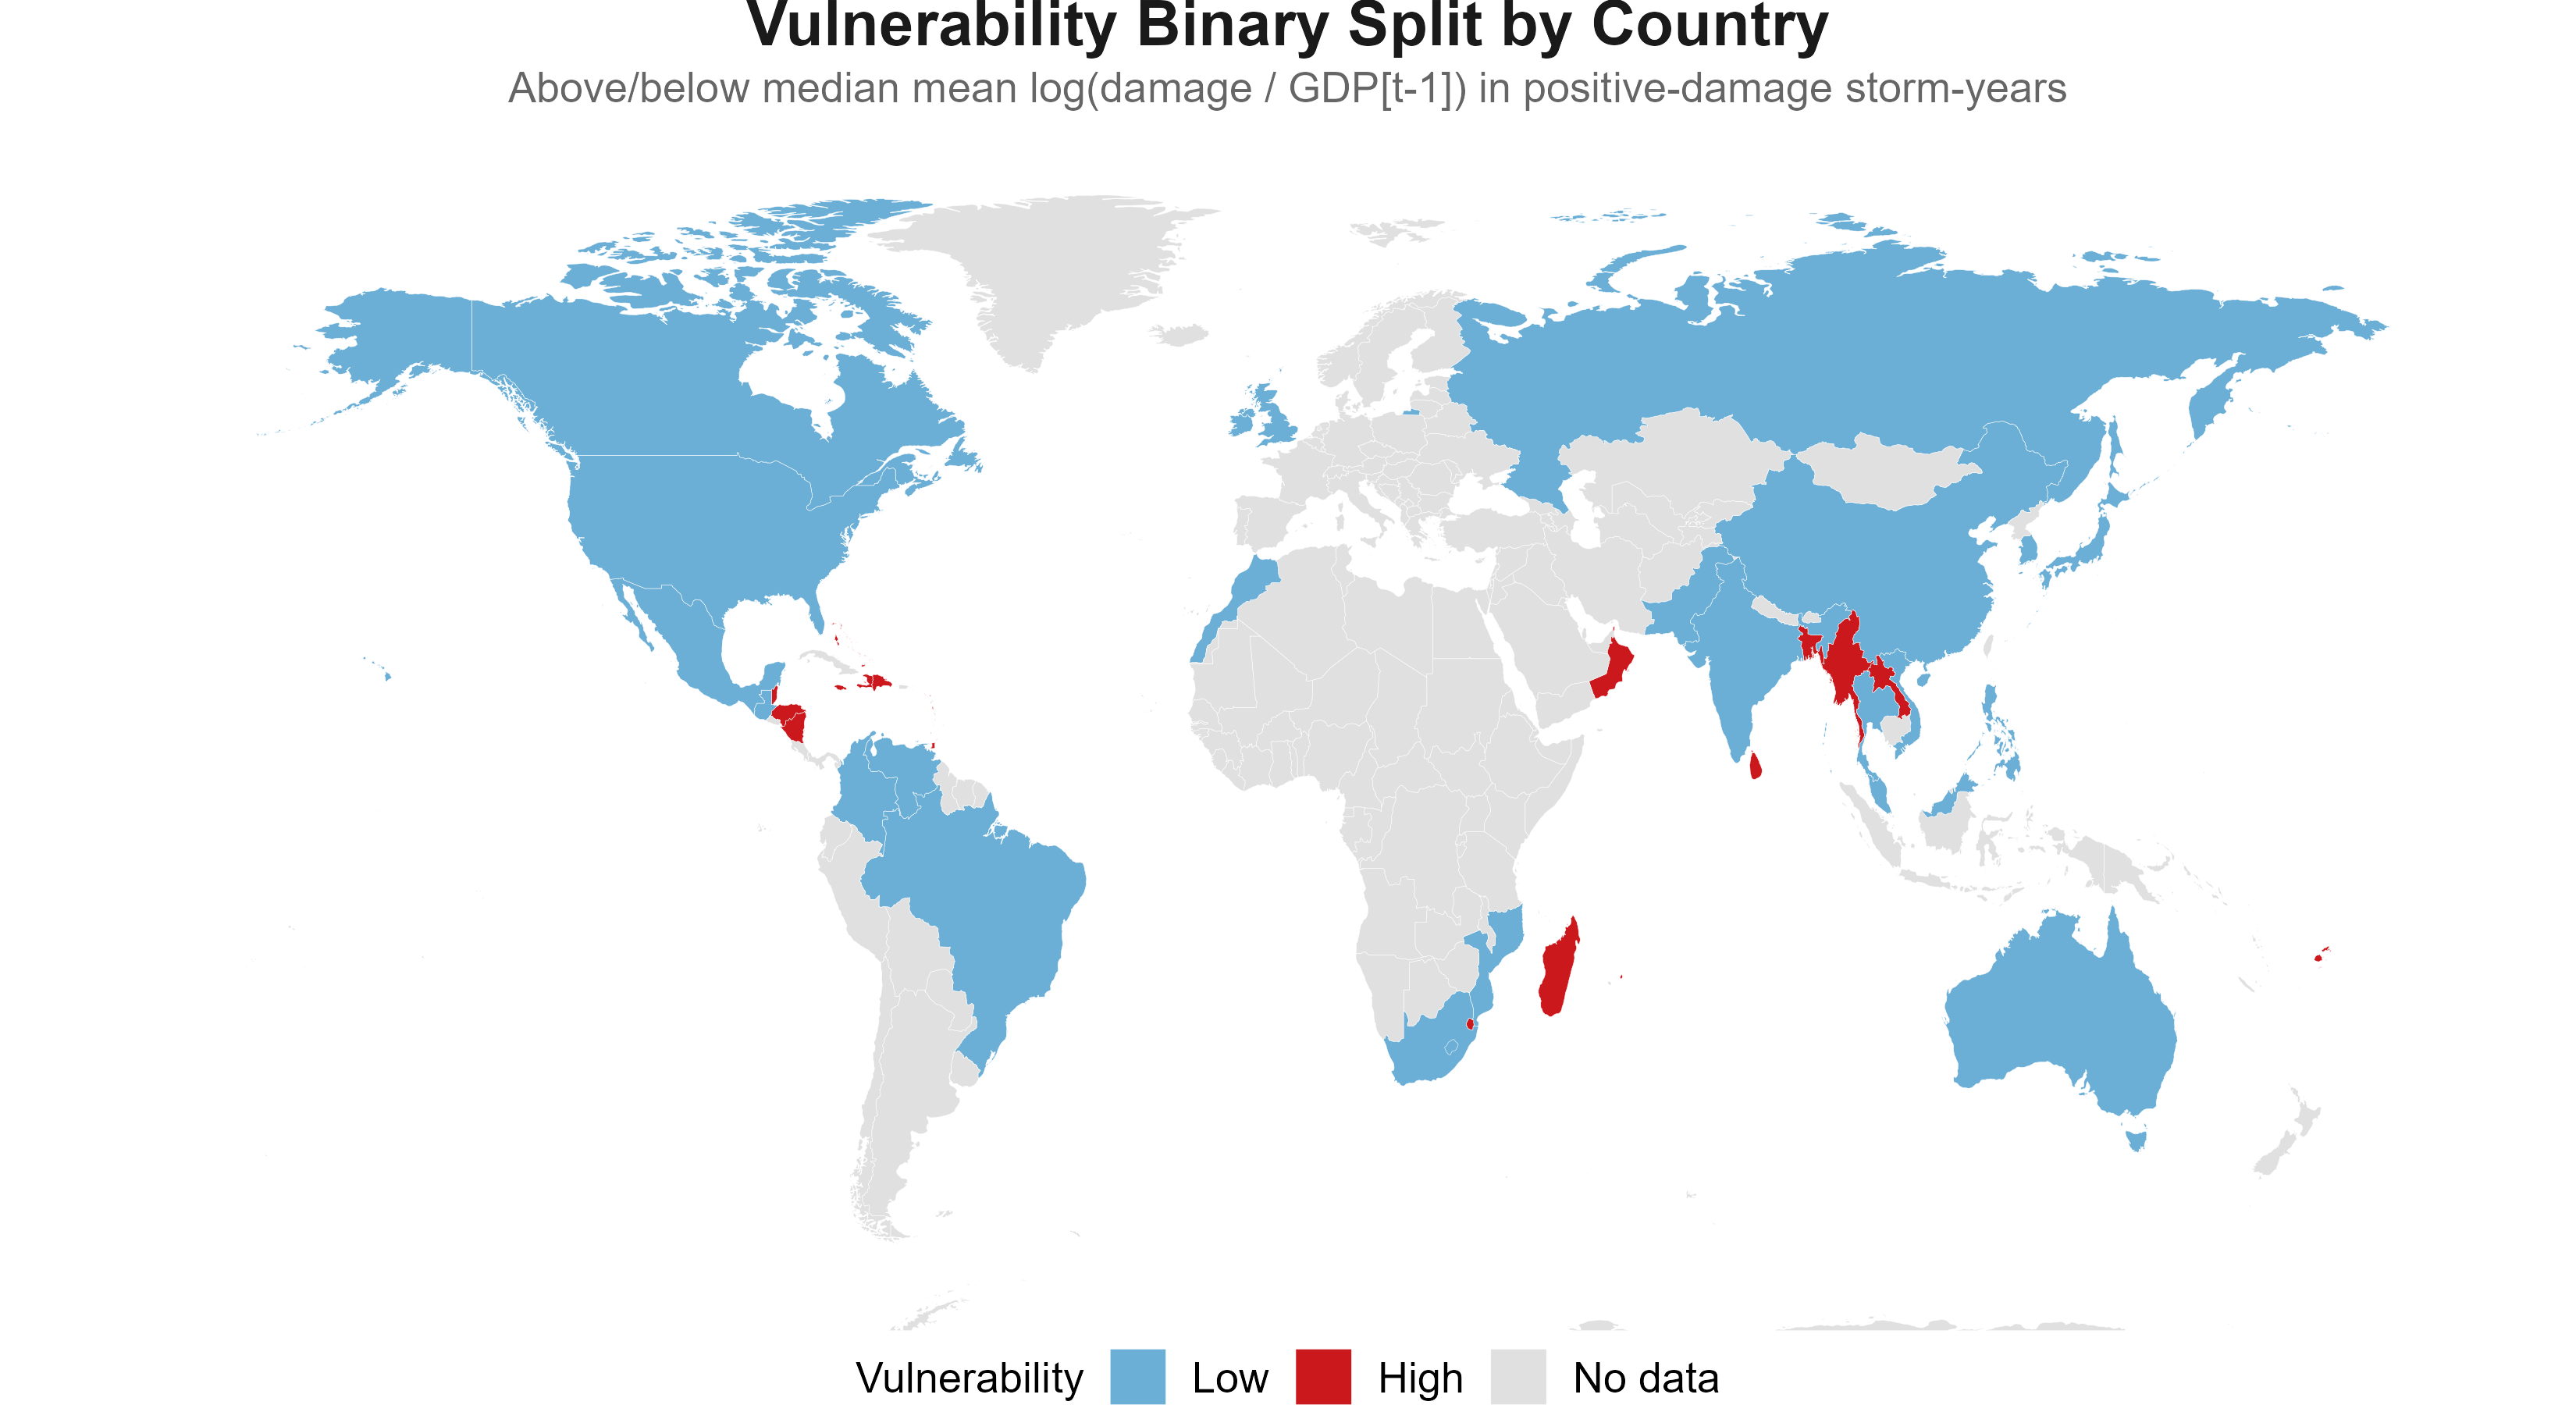
\includegraphics[width=0.95\textwidth,height=0.72\textheight,keepaspectratio]{figures/reconcile_vuln_map.png}

\smallskip\small
Countries shaded by binary vulnerability group (above/below median $v_i$).
High-vulnerability countries (red) concentrate in South and South-East Asia,
the Caribbean, and the Pacific.
Grey = no positive-damage storm record in EMDAT, 1970--2015.
\end{frame}

\begin{frame}{Balance Check: Is Tercile Assignment Quasi-Random?}
\centering
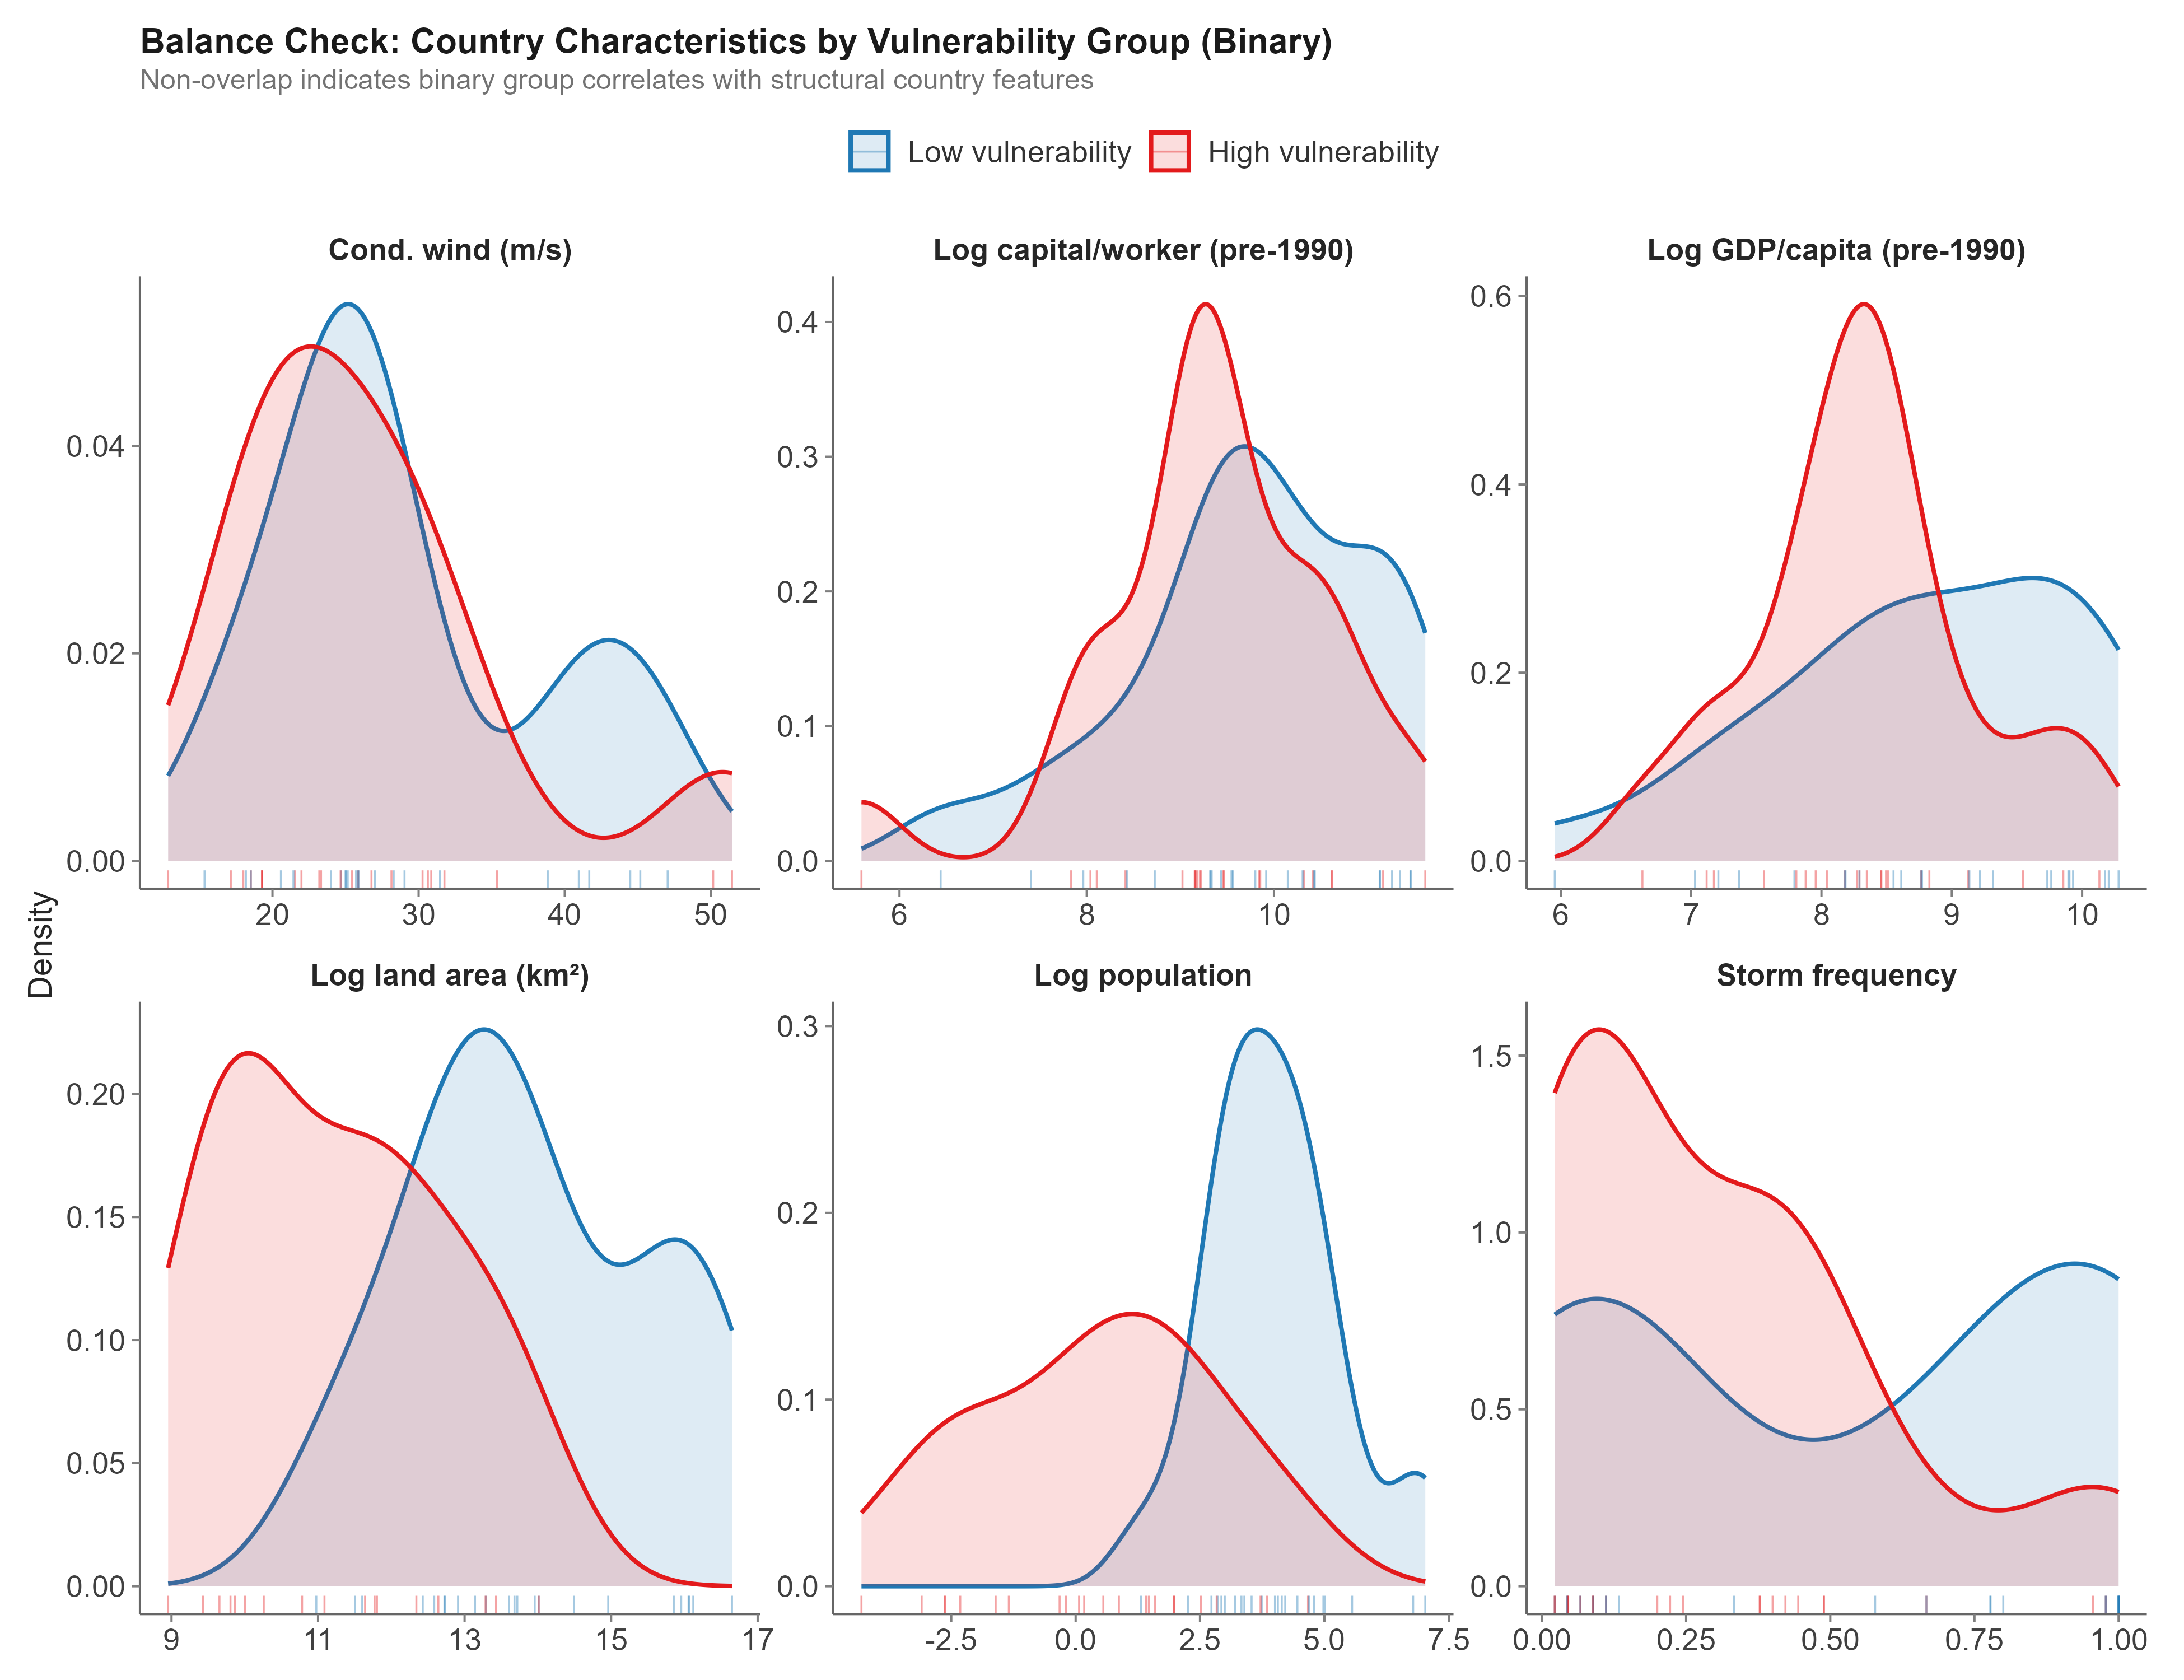
\includegraphics[width=0.95\textwidth,height=0.72\textheight,keepaspectratio]{figures/reconcile_balance.png}

\smallskip\small
Kernel density of pre-determined country characteristics (GDP/capita, population,
land area, storm frequency, conditional wind intensity, capital per worker) by binary group.
Systematic separation indicates the binary split proxies structural features
(income, geography, size) rather than pure damage vulnerability ---
relevant for interpreting the between-country identification in H2.
\end{frame}

\begin{frame}{EDA: Regional Composition by Vulnerability Group}
\centering
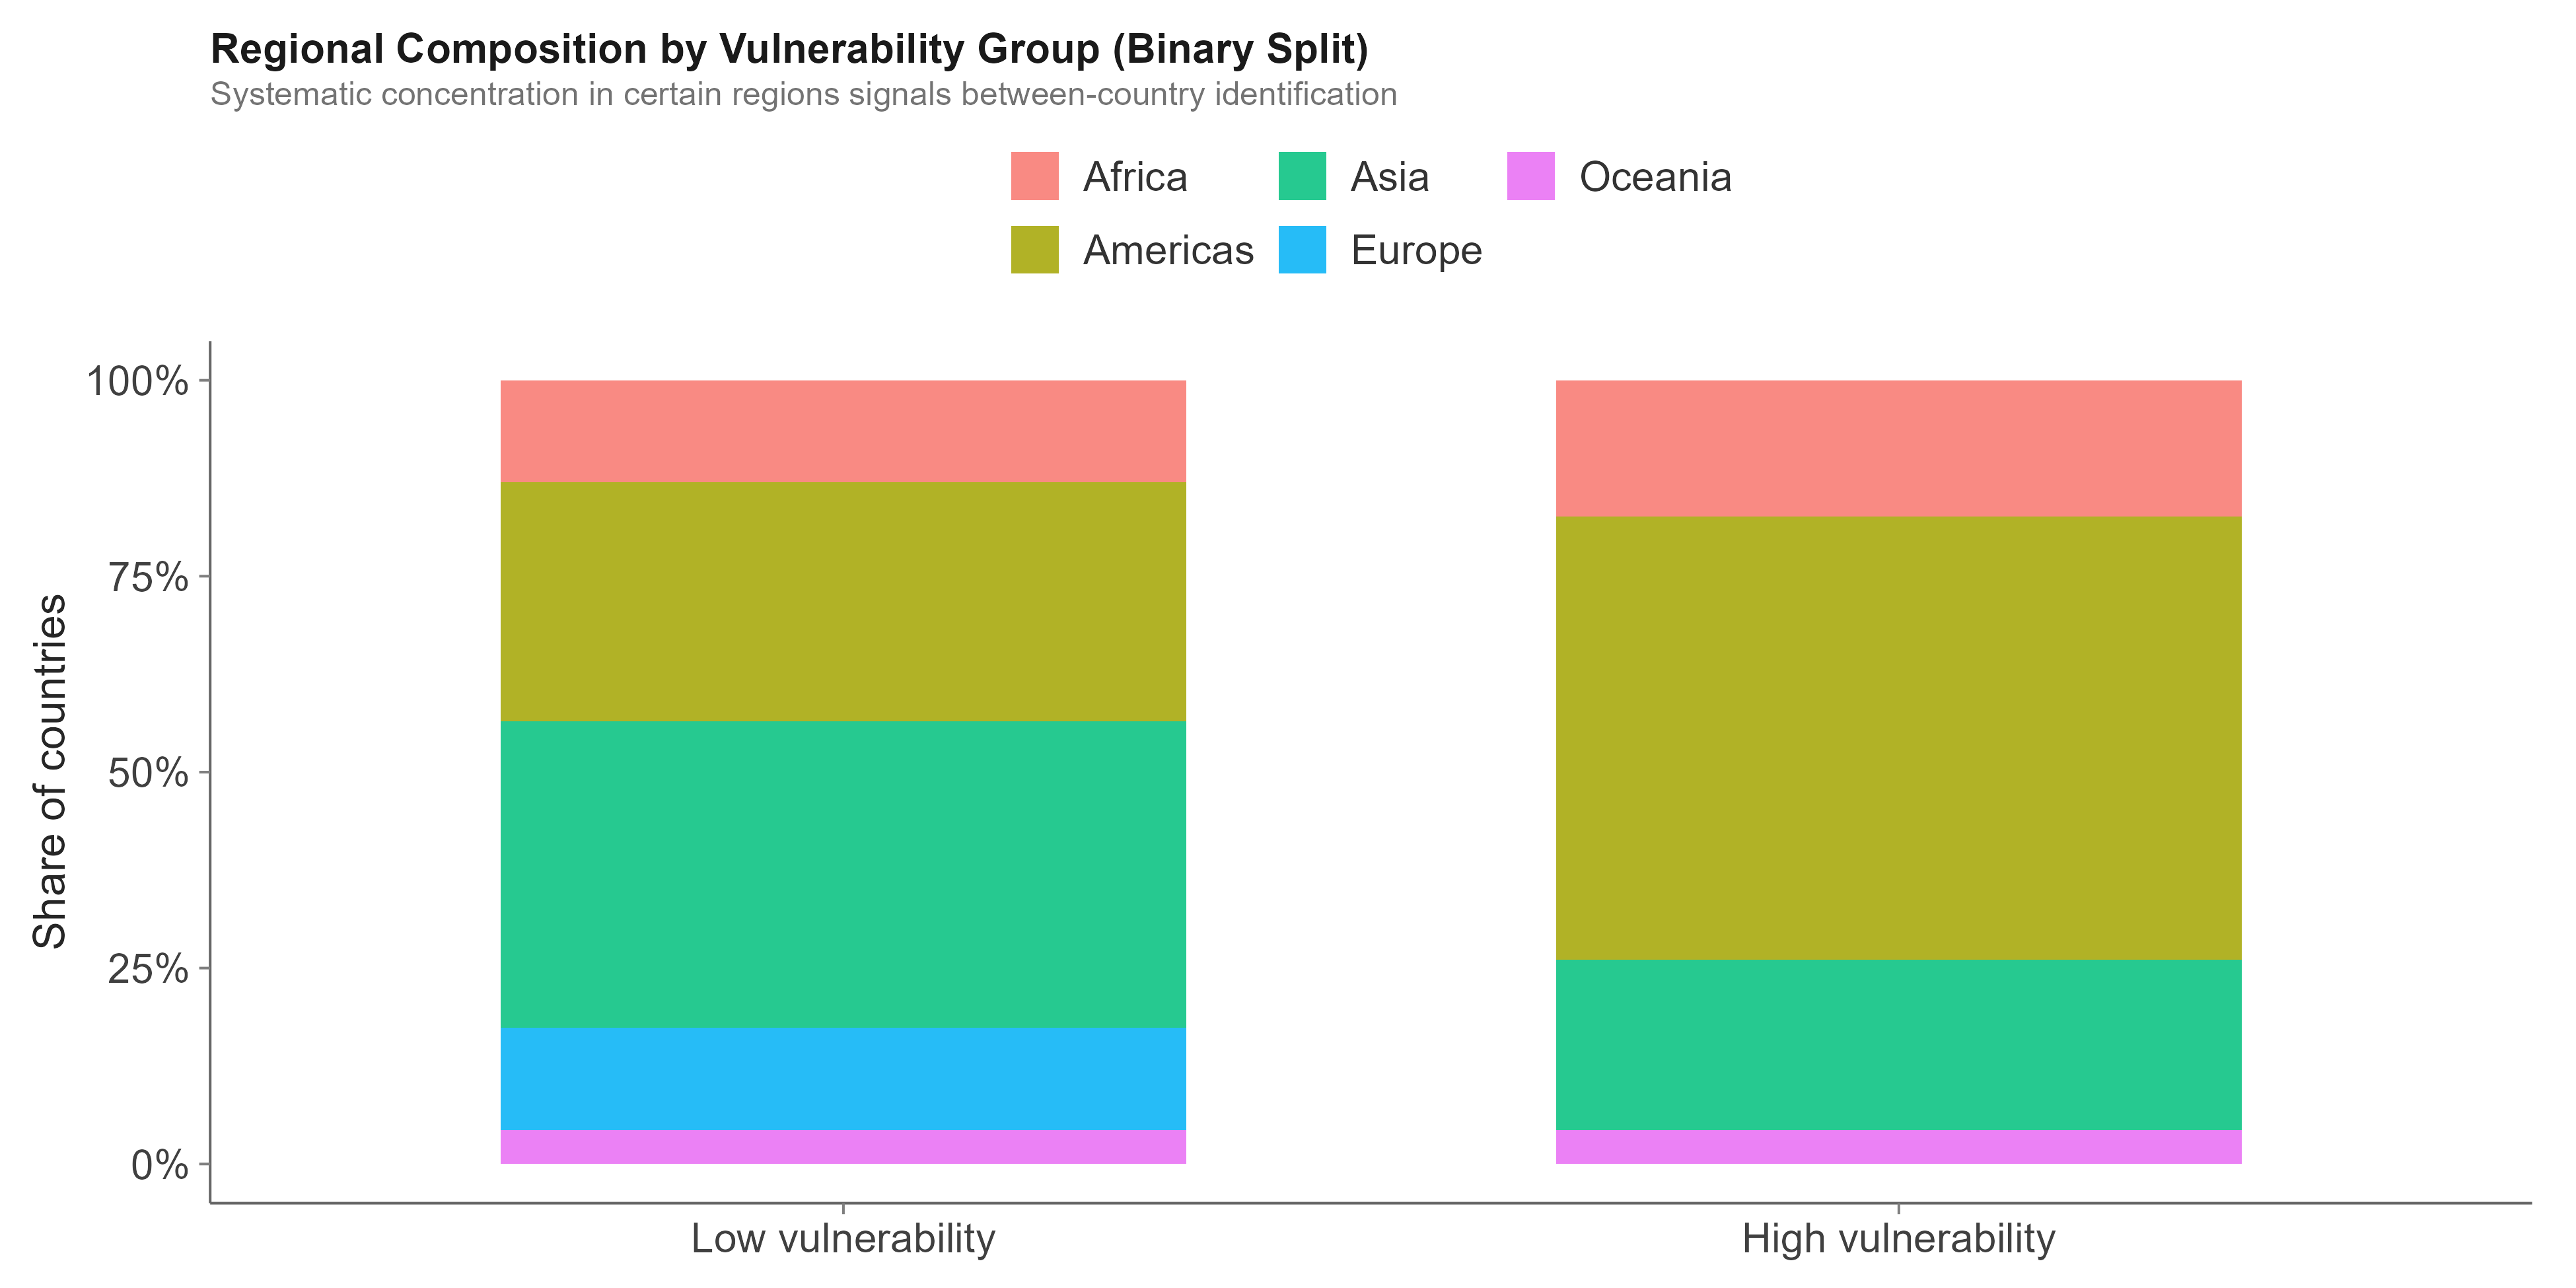
\includegraphics[width=0.75\textwidth,height=0.68\textheight,keepaspectratio]{figures/reconcile_composition.png}

\smallskip\small
Share of countries by continent within each vulnerability group.
Systematic concentration in Asia/Pacific for High vulnerability reflects
the geography of cyclone exposure rather than pure damage vulnerability.
\end{frame}

\begin{frame}{Direct Comparison: State-Dep vs Tercile LP}
\centering
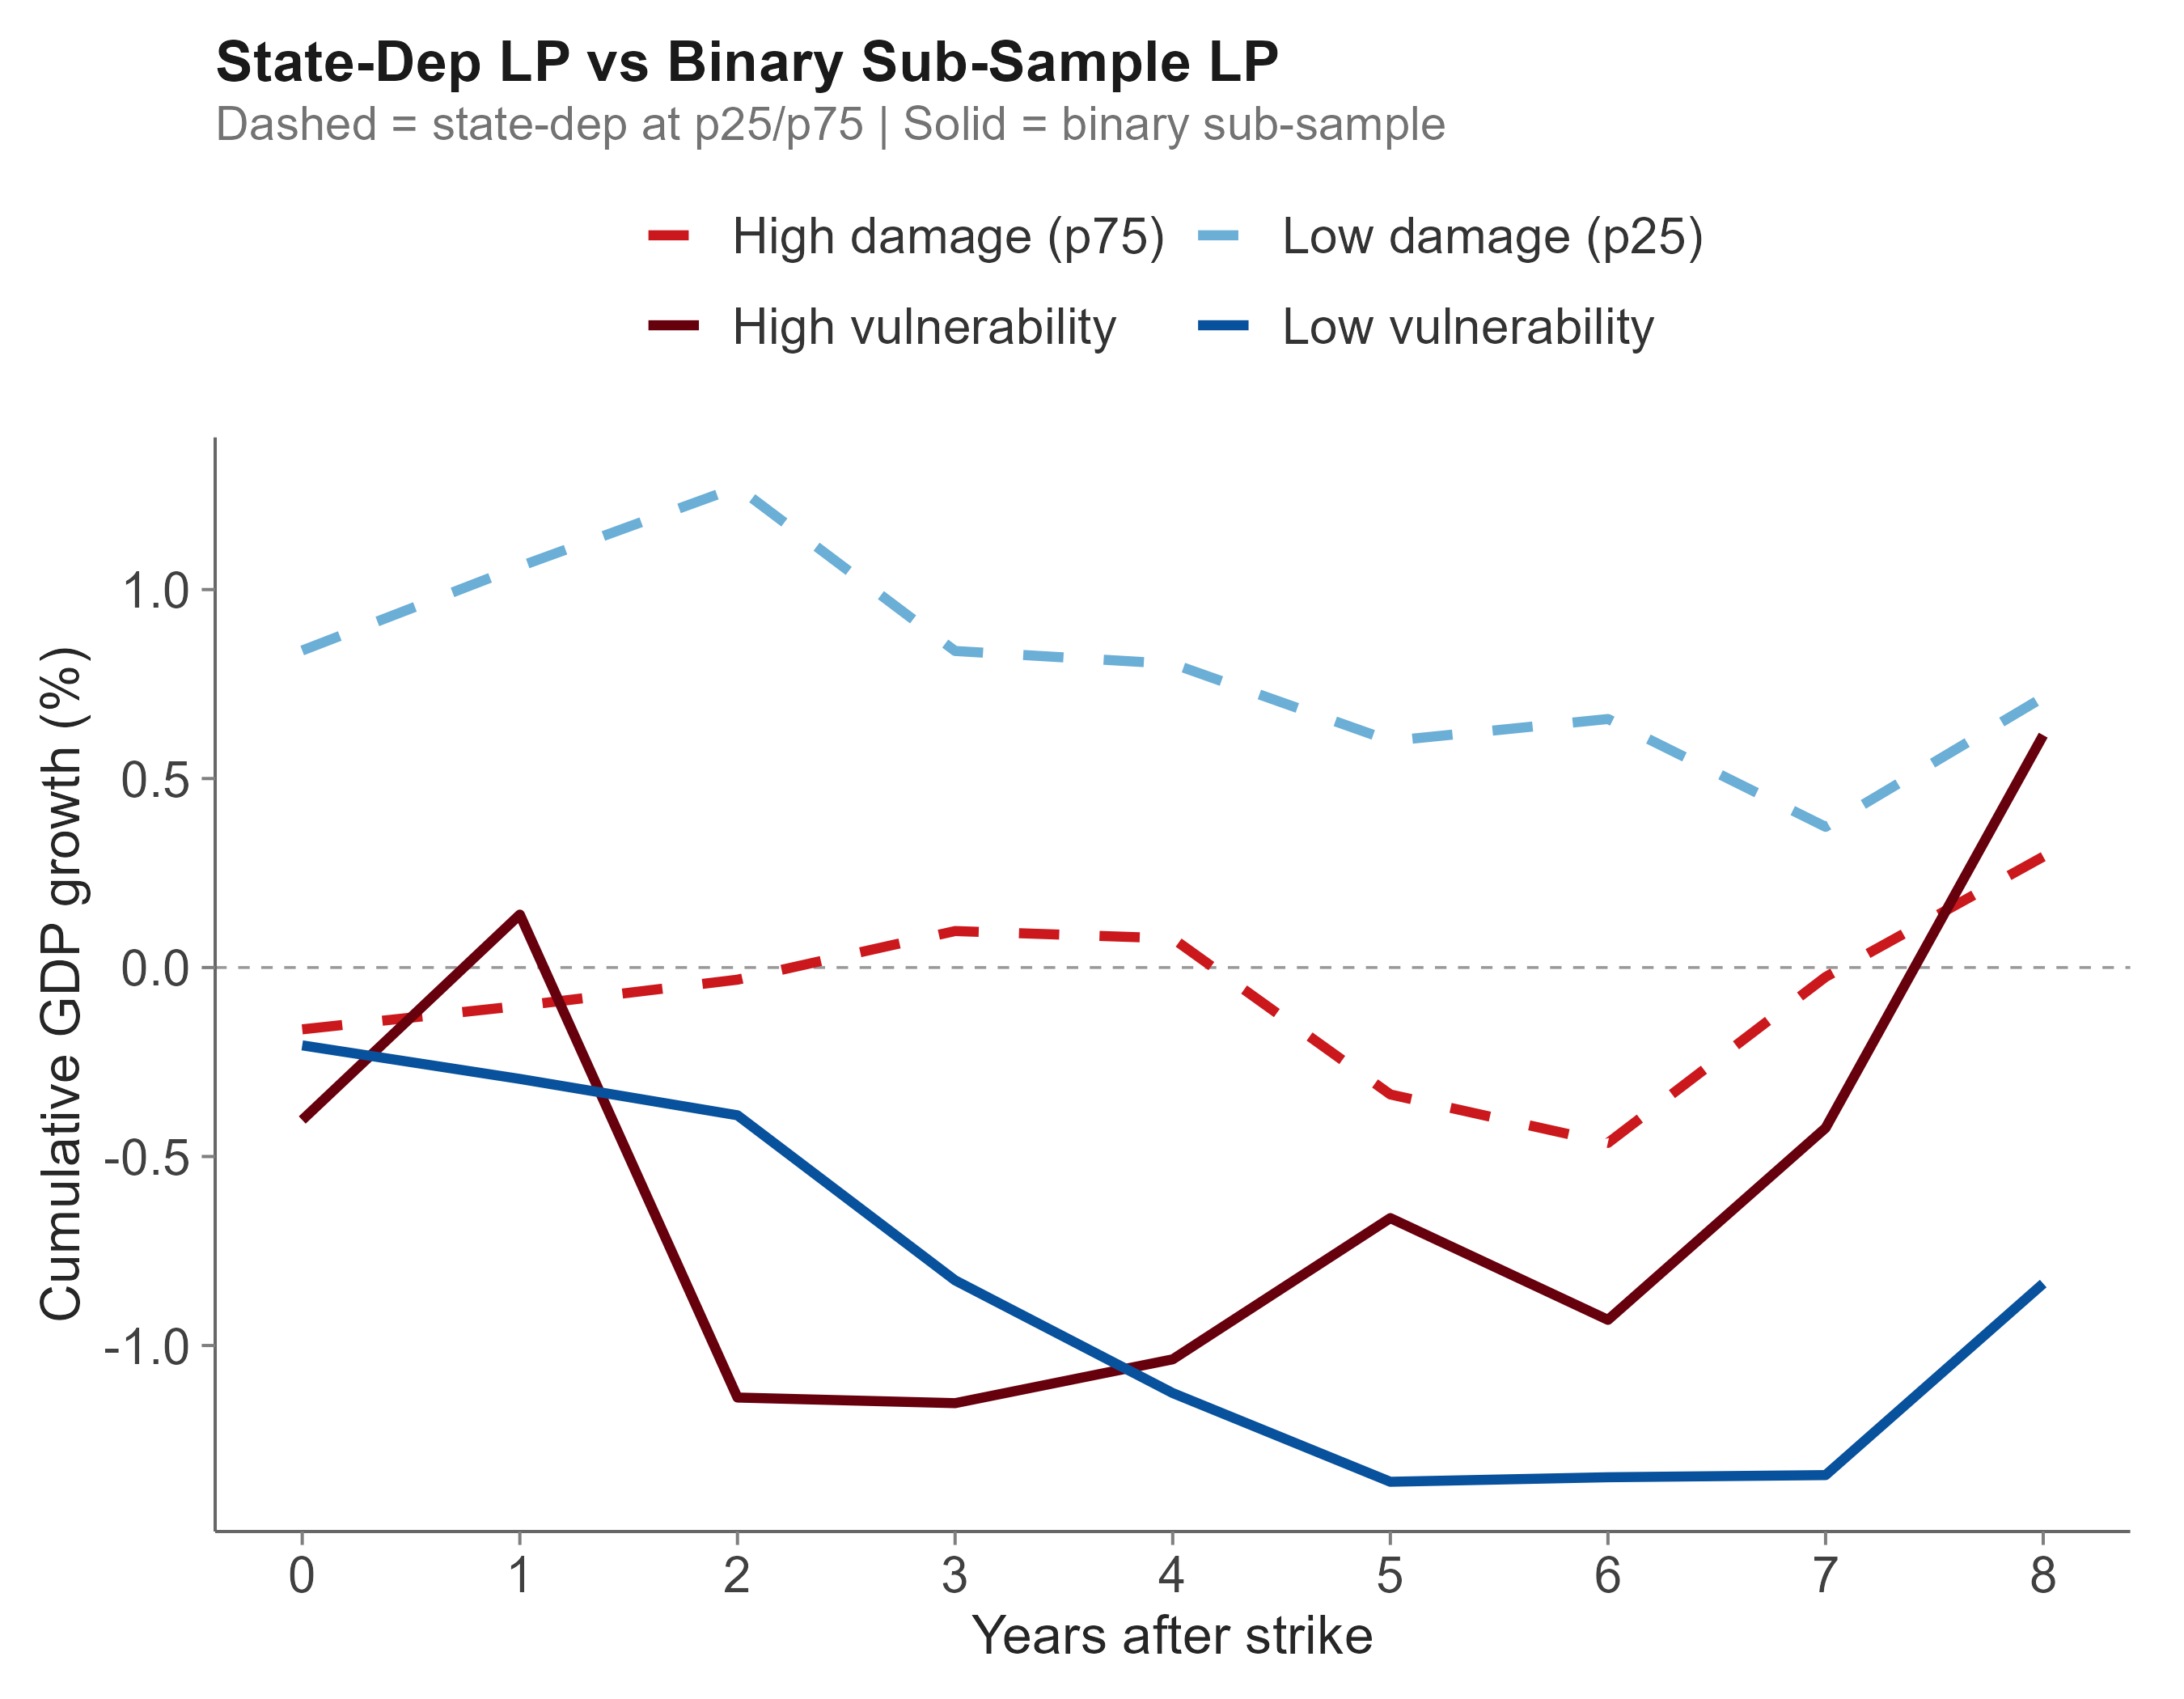
\includegraphics[width=0.82\textwidth,height=0.70\textheight,keepaspectratio]{figures/reconcile_overlay.png}

\smallskip\small
Dashed lines: state-dep LP evaluated at global p10/p50/p90 of contemporaneous
$\log(D_t/\text{GDP}_{t-1})$.
Solid lines: tercile sub-sample LP (all years within each tercile).
Agreement in \emph{ranking} with disagreement in \emph{level} points to
\textbf{H1} or \textbf{H2}; disagreement in ranking points to \textbf{H3}.
\end{frame}

\begin{frame}{H1 -- Storm-Years Only: Tercile LP}
\centering
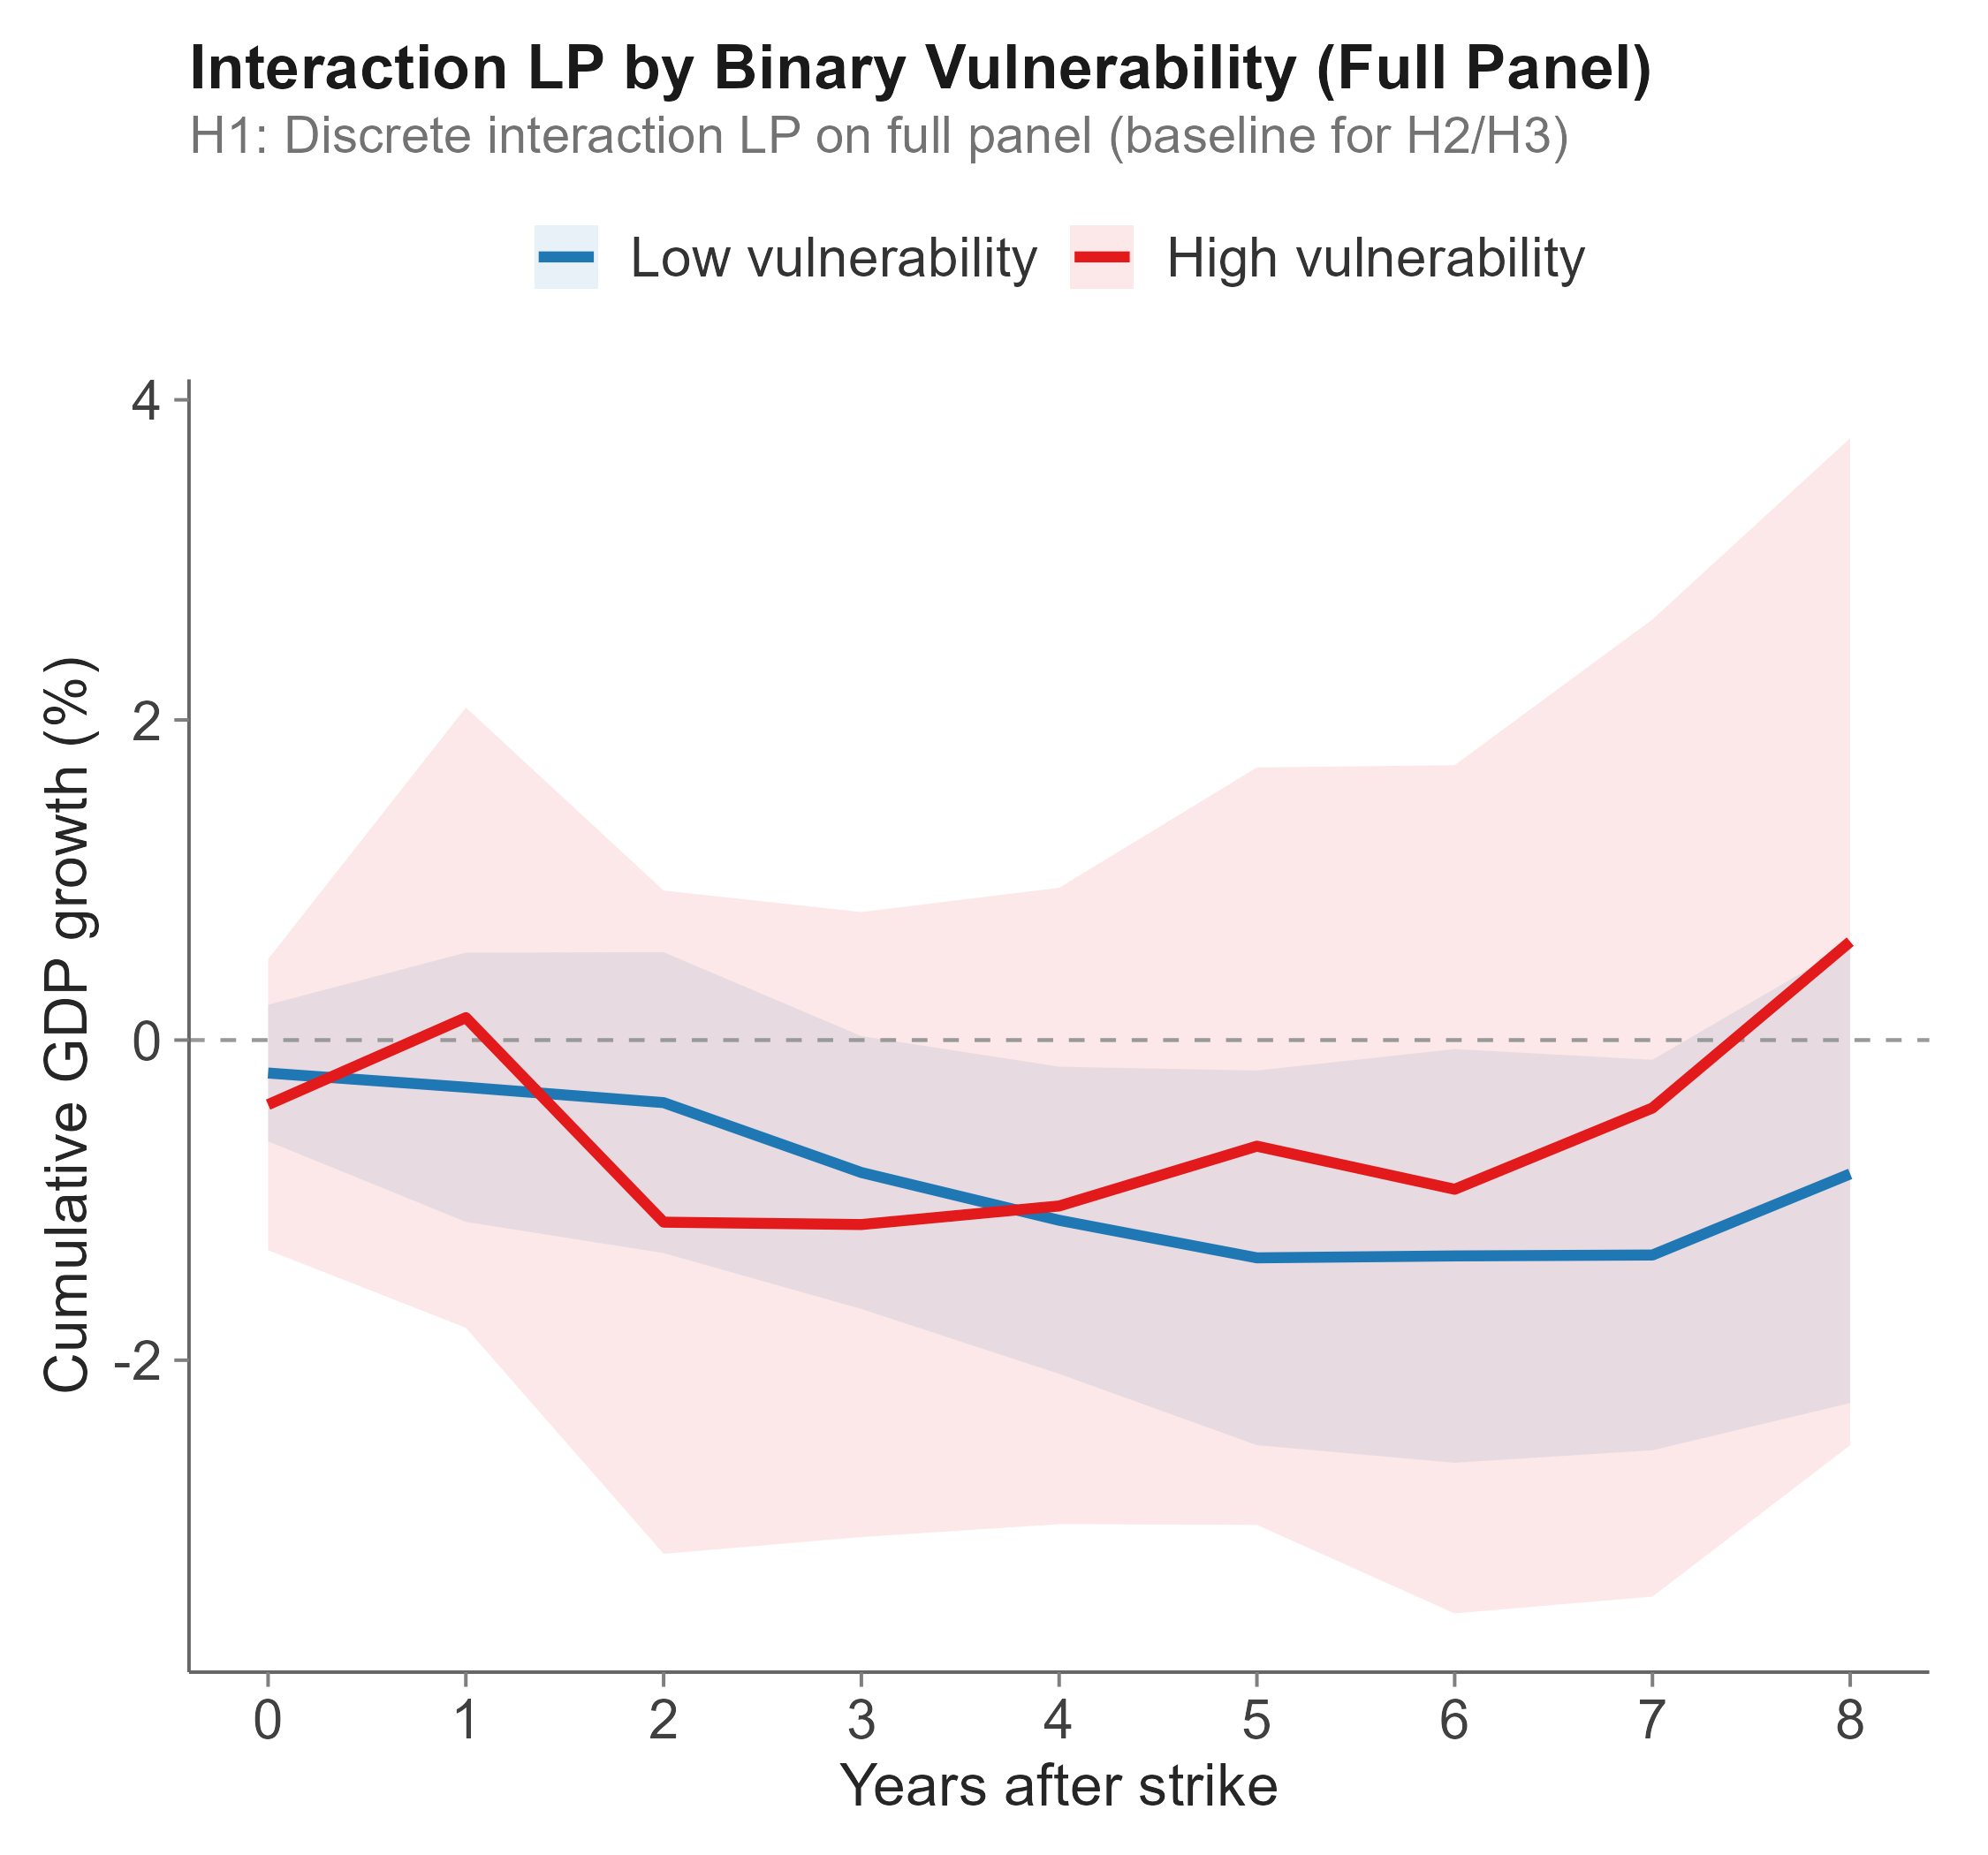
\includegraphics[width=0.82\textwidth,height=0.70\textheight,keepaspectratio]{figures/reconcile_stormyears.png}

\smallskip\small
Full-panel interaction LP (\texttt{lp\_panel\_inter}) using \texttt{i(damage\_binary, wind\_cat1plus)}.
Gives separate wind-on-GDP slopes for Low and High vulnerability directly from a
single pooled regression.  Serves as the discrete-interaction baseline for comparing
with H2 (time-invariant state) and H3 (continuous state-dep at p25/p75).
\end{frame}

\begin{frame}{H2 -- Time-Invariant State Variable}
\centering
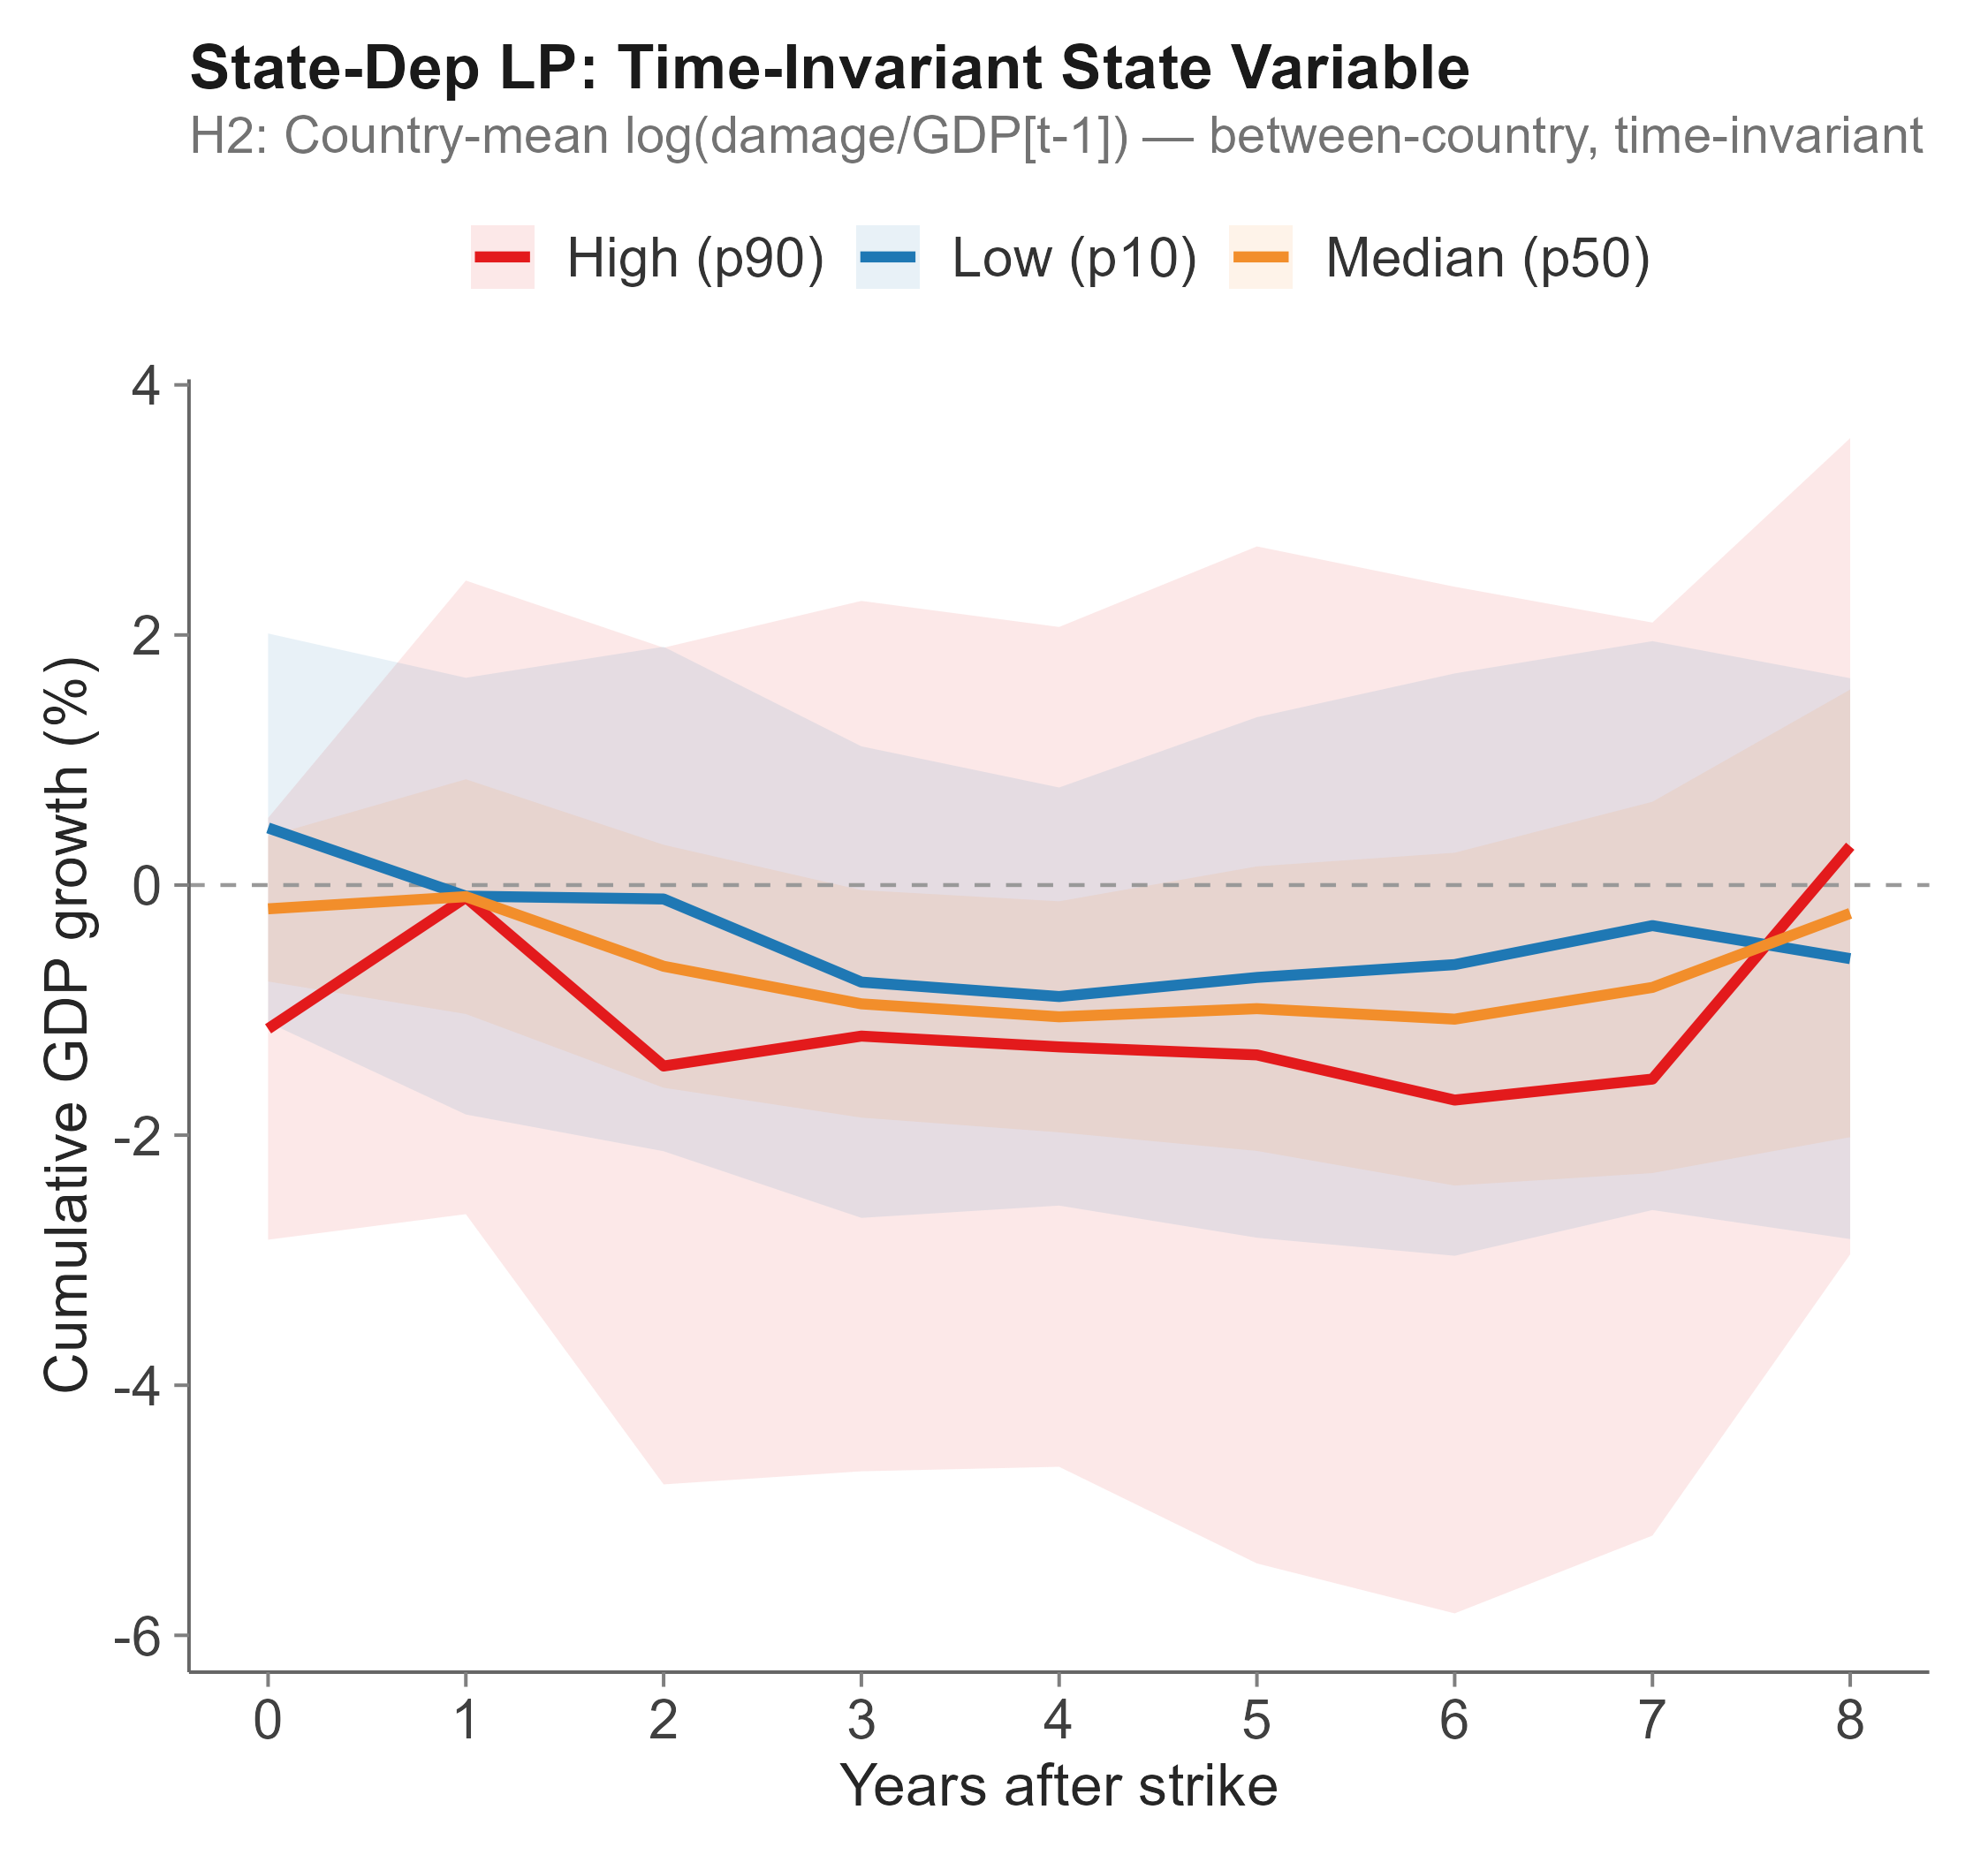
\includegraphics[width=0.82\textwidth,height=0.70\textheight,keepaspectratio]{figures/reconcile_timeinvariant.png}

\smallskip\small
State-dep LP re-estimated replacing contemporaneous $\log(D_t/\text{GDP}_{t-1})$
with each country's long-run mean over storm-years (time-invariant).
A time-invariant state variable captures between-country differences,
bringing the state-dep LP conceptually in line with the tercile approach.
Convergence here isolates \textbf{H2} as a key driver.
\end{frame}

\begin{frame}{H3 -- State-Dep Evaluated at Tercile Boundaries}
\centering
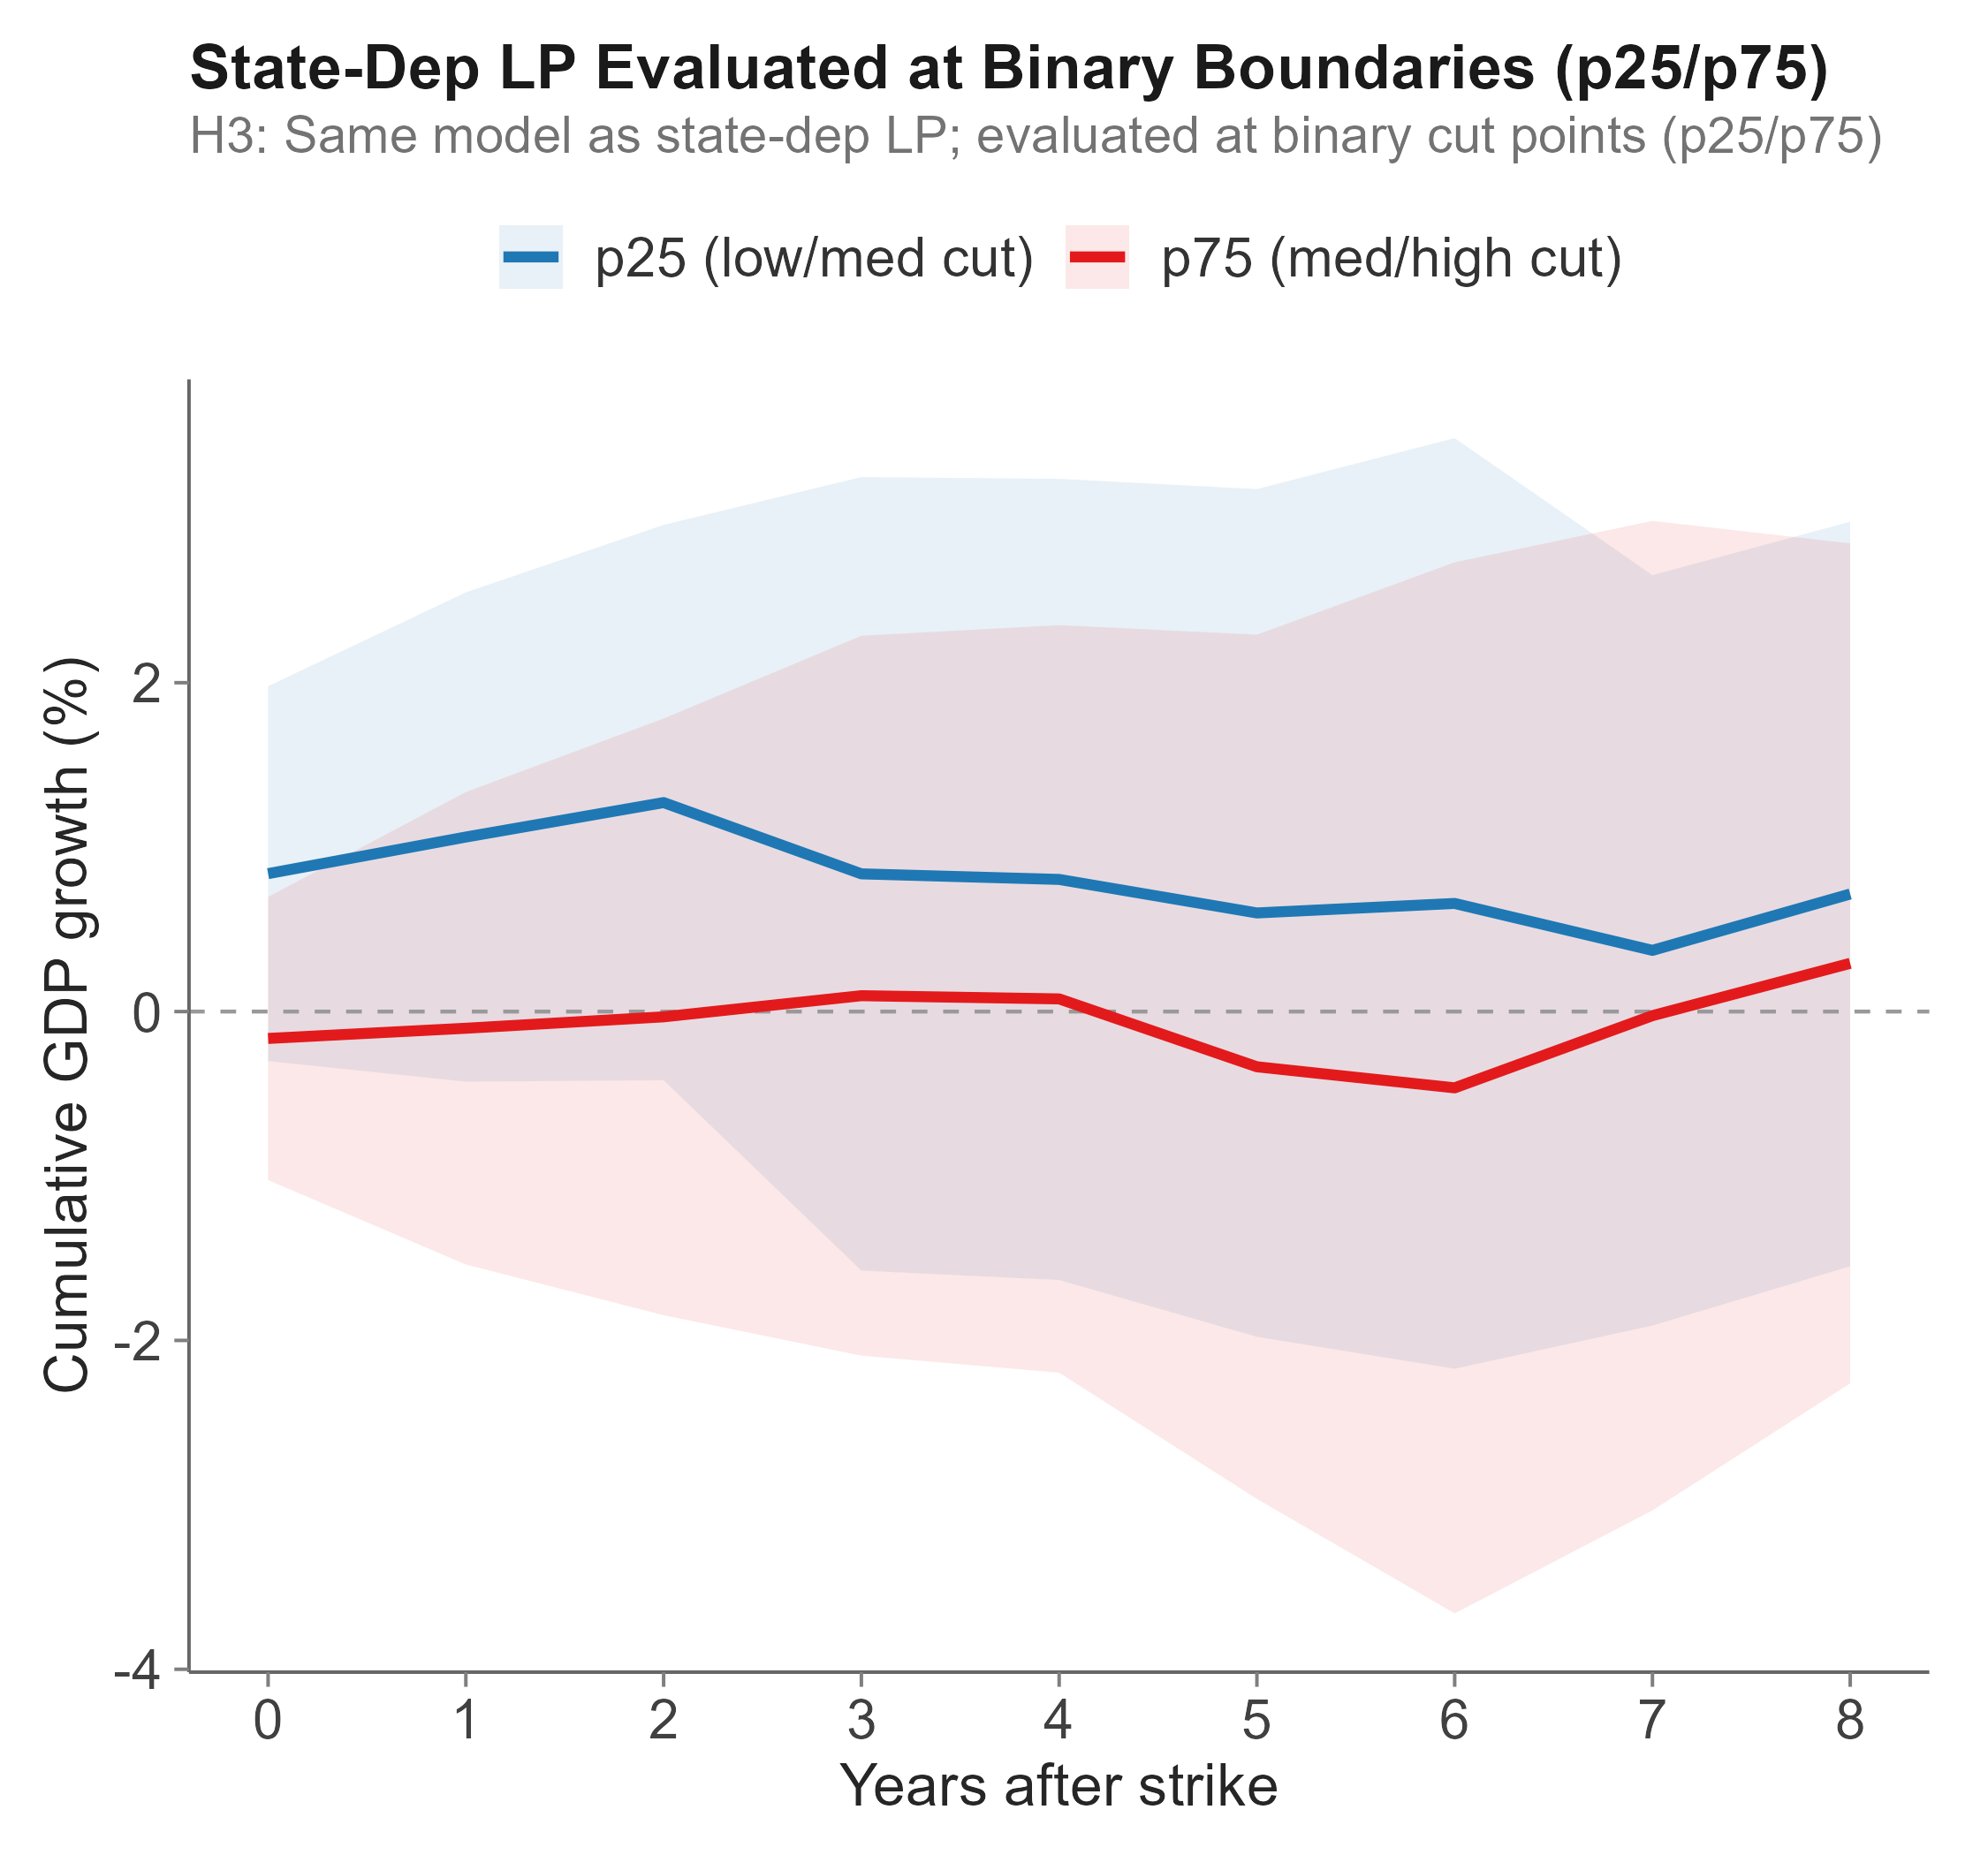
\includegraphics[width=0.82\textwidth,height=0.70\textheight,keepaspectratio]{figures/reconcile_tercile_cuts.png}

\smallskip\small
Same state-dep LP model; marginal effects evaluated at the tercile cut
points p33 and p67 rather than p10/p90.
If \textbf{H3} (functional form) matters, results at p33/p67 should bracket
the tercile LP estimates more closely than the wide p10/p90 range.
\end{frame}

\begin{frame}{Robustness: Ever-Treated Countries}
\centering
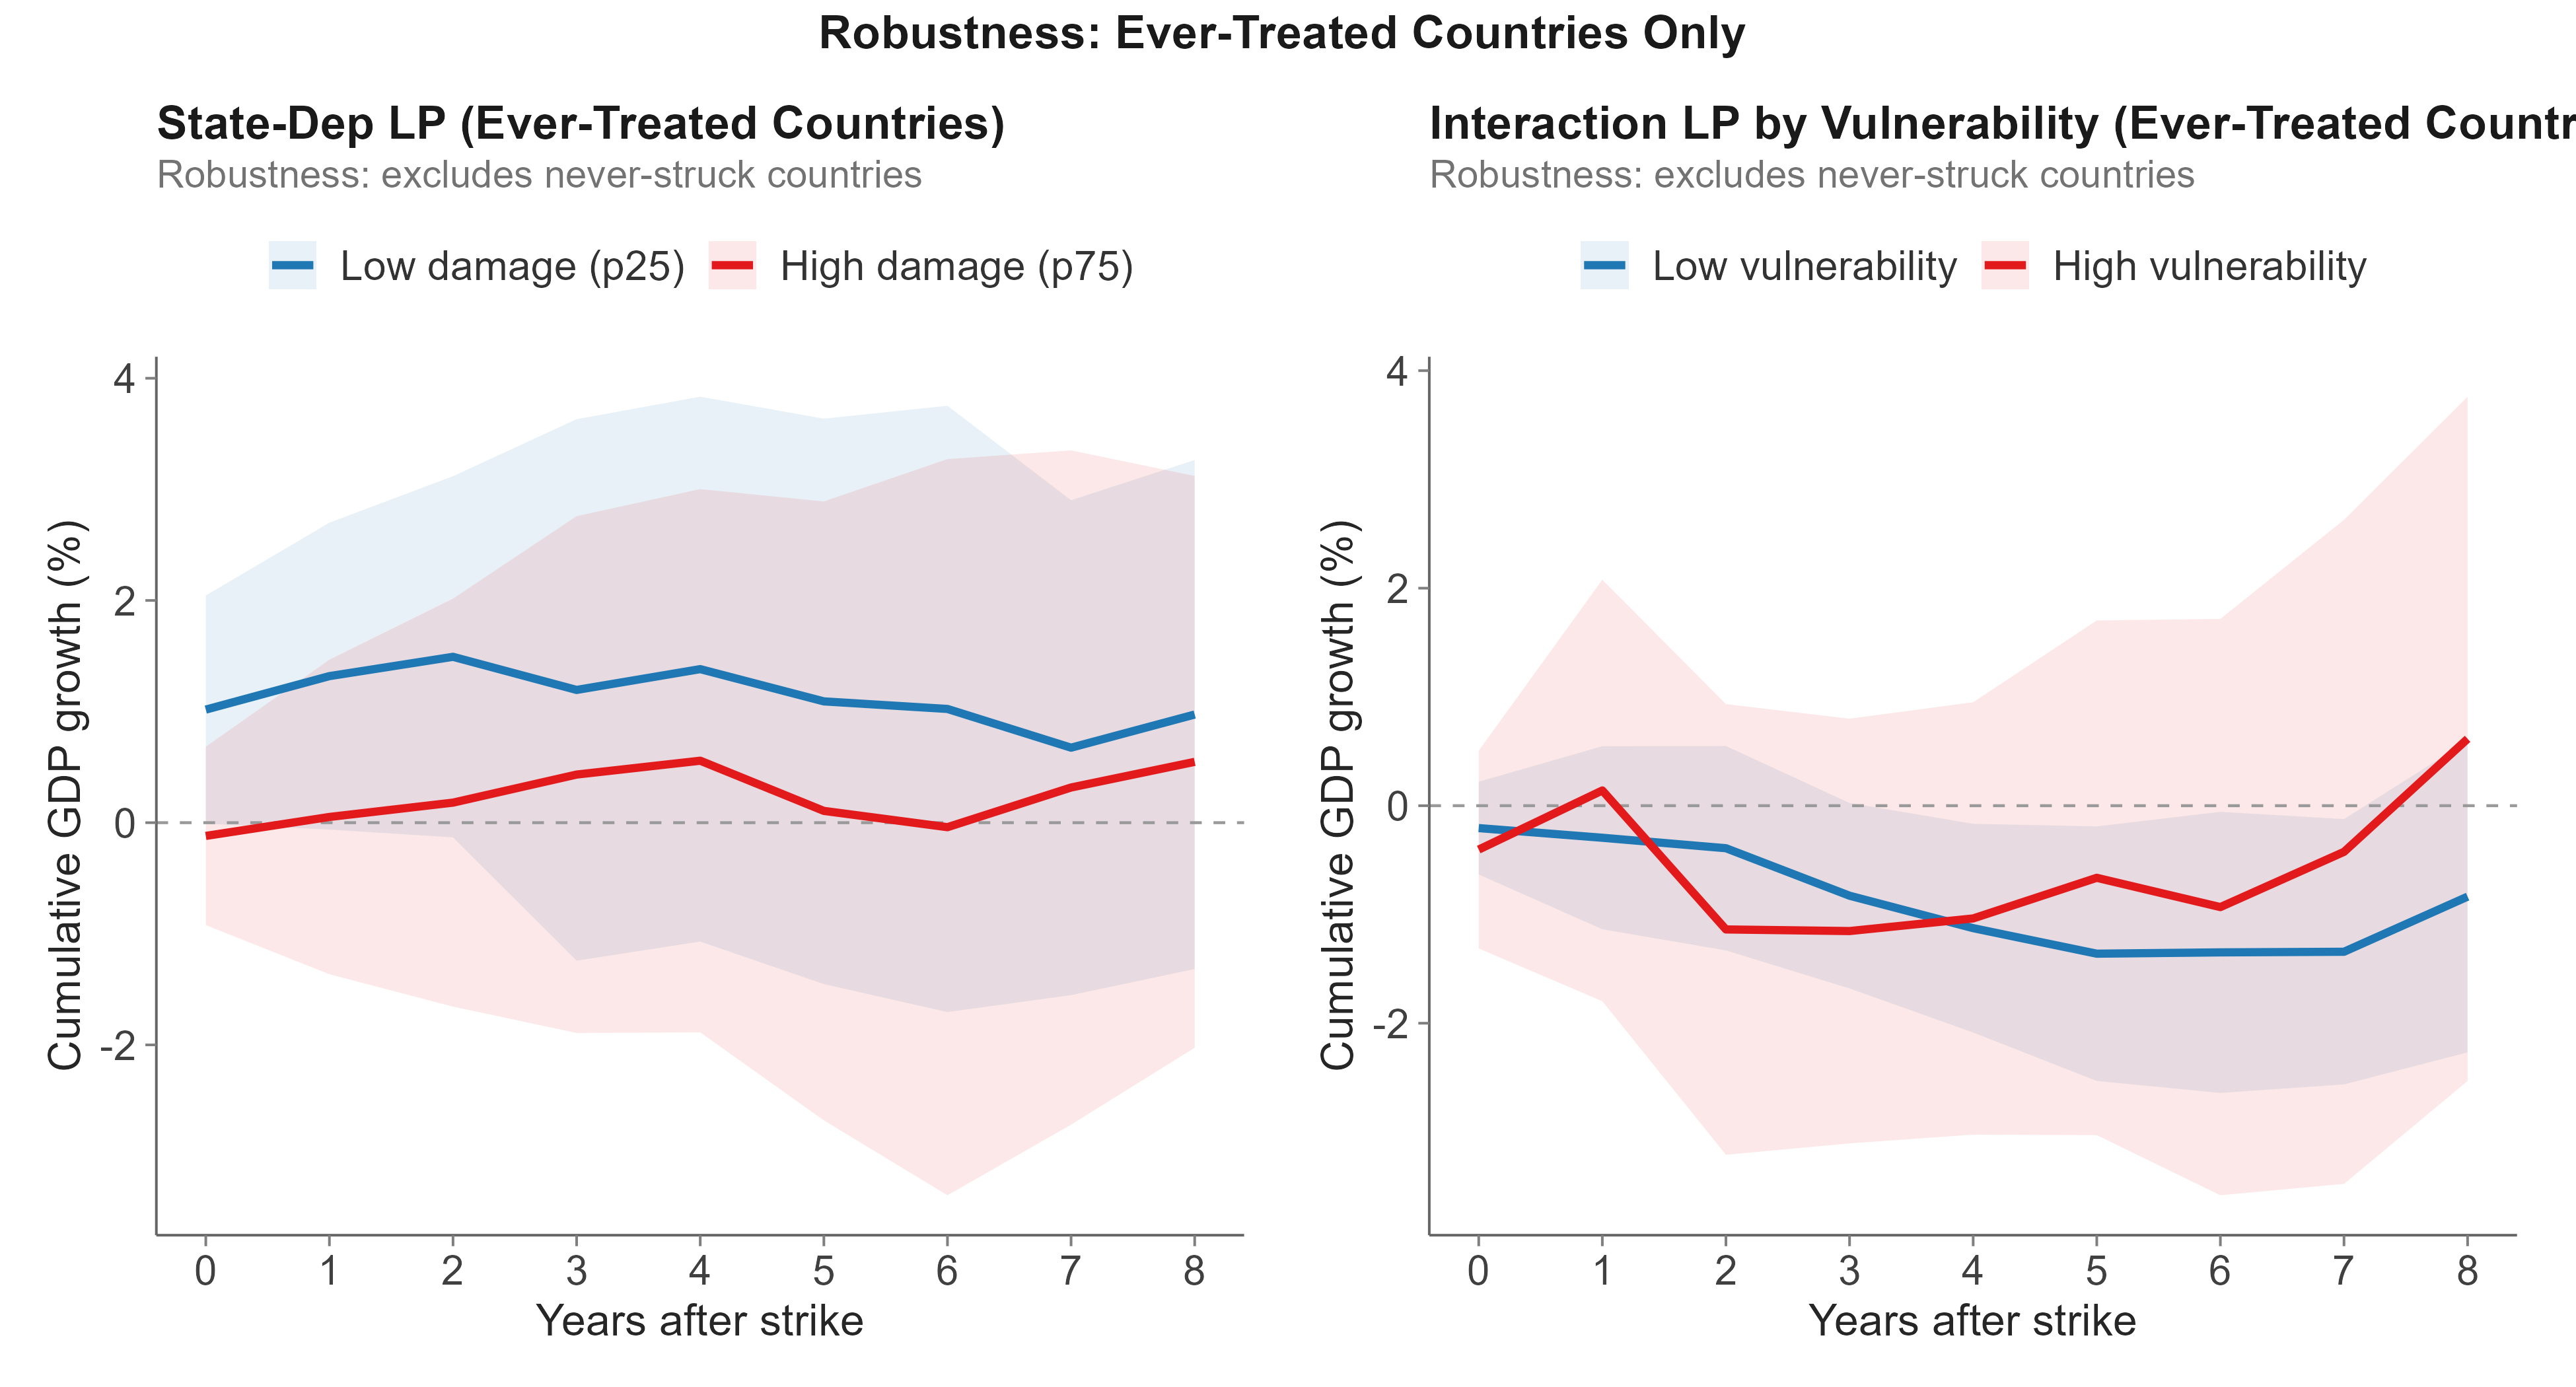
\includegraphics[width=0.96\textwidth,height=0.72\textheight,keepaspectratio]{figures/reconcile_ever_treated.png}

\smallskip\small
Both heterogeneity approaches re-estimated on countries that were ever struck
by any cyclone ($\text{maxwind}>0$ in at least one year).
Never-struck countries contribute only to fixed-effect precision in the full panel;
excluding them tests whether they distort the heterogeneity estimates.
\end{frame}

% ===============================================================
\section{Takeaways}
% ===============================================================
{\hideframenumber\begin{frame}\sectionpage\end{frame}\showframenumber}

\begin{frame}{Summary}
\begin{enumerate}
  \item \textbf{Direct losses scale with wind.}  Both $\log(\text{damage}/\text{GDP}_{t-1})$
        and $\log(\text{deaths/pop})$ increase monotonically from Cat~1 to
        Cat~3$+$, with mortality losses proportionally steeper.

  \medskip
  \item \textbf{GDP drag is intensity-graded.}  Cat~3$+$ strikes produce
        deeper and more persistent GDP declines than Cat~1$+$ events;
        effects accumulate over 3--5 years.

  \medskip
  \item \textbf{Prior damage amplifies the GDP channel.}
        The state-dependent LP shows that the same Cat~1$+$ shock
        generates substantially larger output losses when contemporaneous
        $\log(\text{damage}/\text{GDP}_{t-1})$ is high, consistent with a
        damage--vulnerability trap.

  \medskip
  \item \textbf{Heterogeneity matters.}
        Country damage vulnerability explains a significant share of
        cross-country variation in GDP responses, over and above
        wind intensity alone.

  \medskip
  \item \textbf{Caveat.}
        EMDAT under-reports damages for small/poor countries;
        true direct losses --- and the amplification channel ---
        may be larger than estimated.
\end{enumerate}
\end{frame}

% =============================================================================
% SUPPLEMENTAL: Adaptation Heterogeneity
% =============================================================================
\appendix

\begin{frame}
\centering
\vfill
{\color{primary!40}\rule{0.35\textwidth}{0.4pt}}\\[1.2em]
{\LARGE\bfseries\color{primary}Supplemental: Adaptation}\\[1.2em]
{\color{primary!40}\rule{0.35\textwidth}{0.4pt}}
\vfill
\end{frame}

\begin{frame}{Measuring Adaptation from Damage Data}

\textbf{Idea:} the within-country slope of log(damage/GDP) on wind speed
measures how much infrastructure amplifies cyclone intensity into economic losses.
\[
  \log(D_{it}/Y_{i,t-1}) = \alpha_i + \beta_i \cdot w_{it} + \varepsilon_{it}
\]

\medskip
\begin{tabular}{@{}lp{8.2cm}@{}}
\toprule
$\hat\beta_i$ & Interpretation \\
\midrule
\textbf{Low / flat} & Damage rises little with wind intensity. \textit{Adapted.} \\[4pt]
\textbf{High / steep} & Each extra m/s translates to much larger losses. \textit{Not adapted.} \\
\bottomrule
\end{tabular}

\medskip
\textbf{Estimation:} linear mixed-effects model with random slopes by country,
estimated on all country-years with positive EMDAT damage (349 obs, 45 countries).
Random slopes are shrunk toward the pooled mean --- prevents small-sample
countries with 1--2 damage obs from driving extreme slope estimates.

\medskip
Countries grouped into \textbf{terciles} of $\hat\beta_i$; GDP IRF
estimated separately for each group.
\end{frame}

\begin{frame}{Country Wind-Damage Elasticities}
\centering
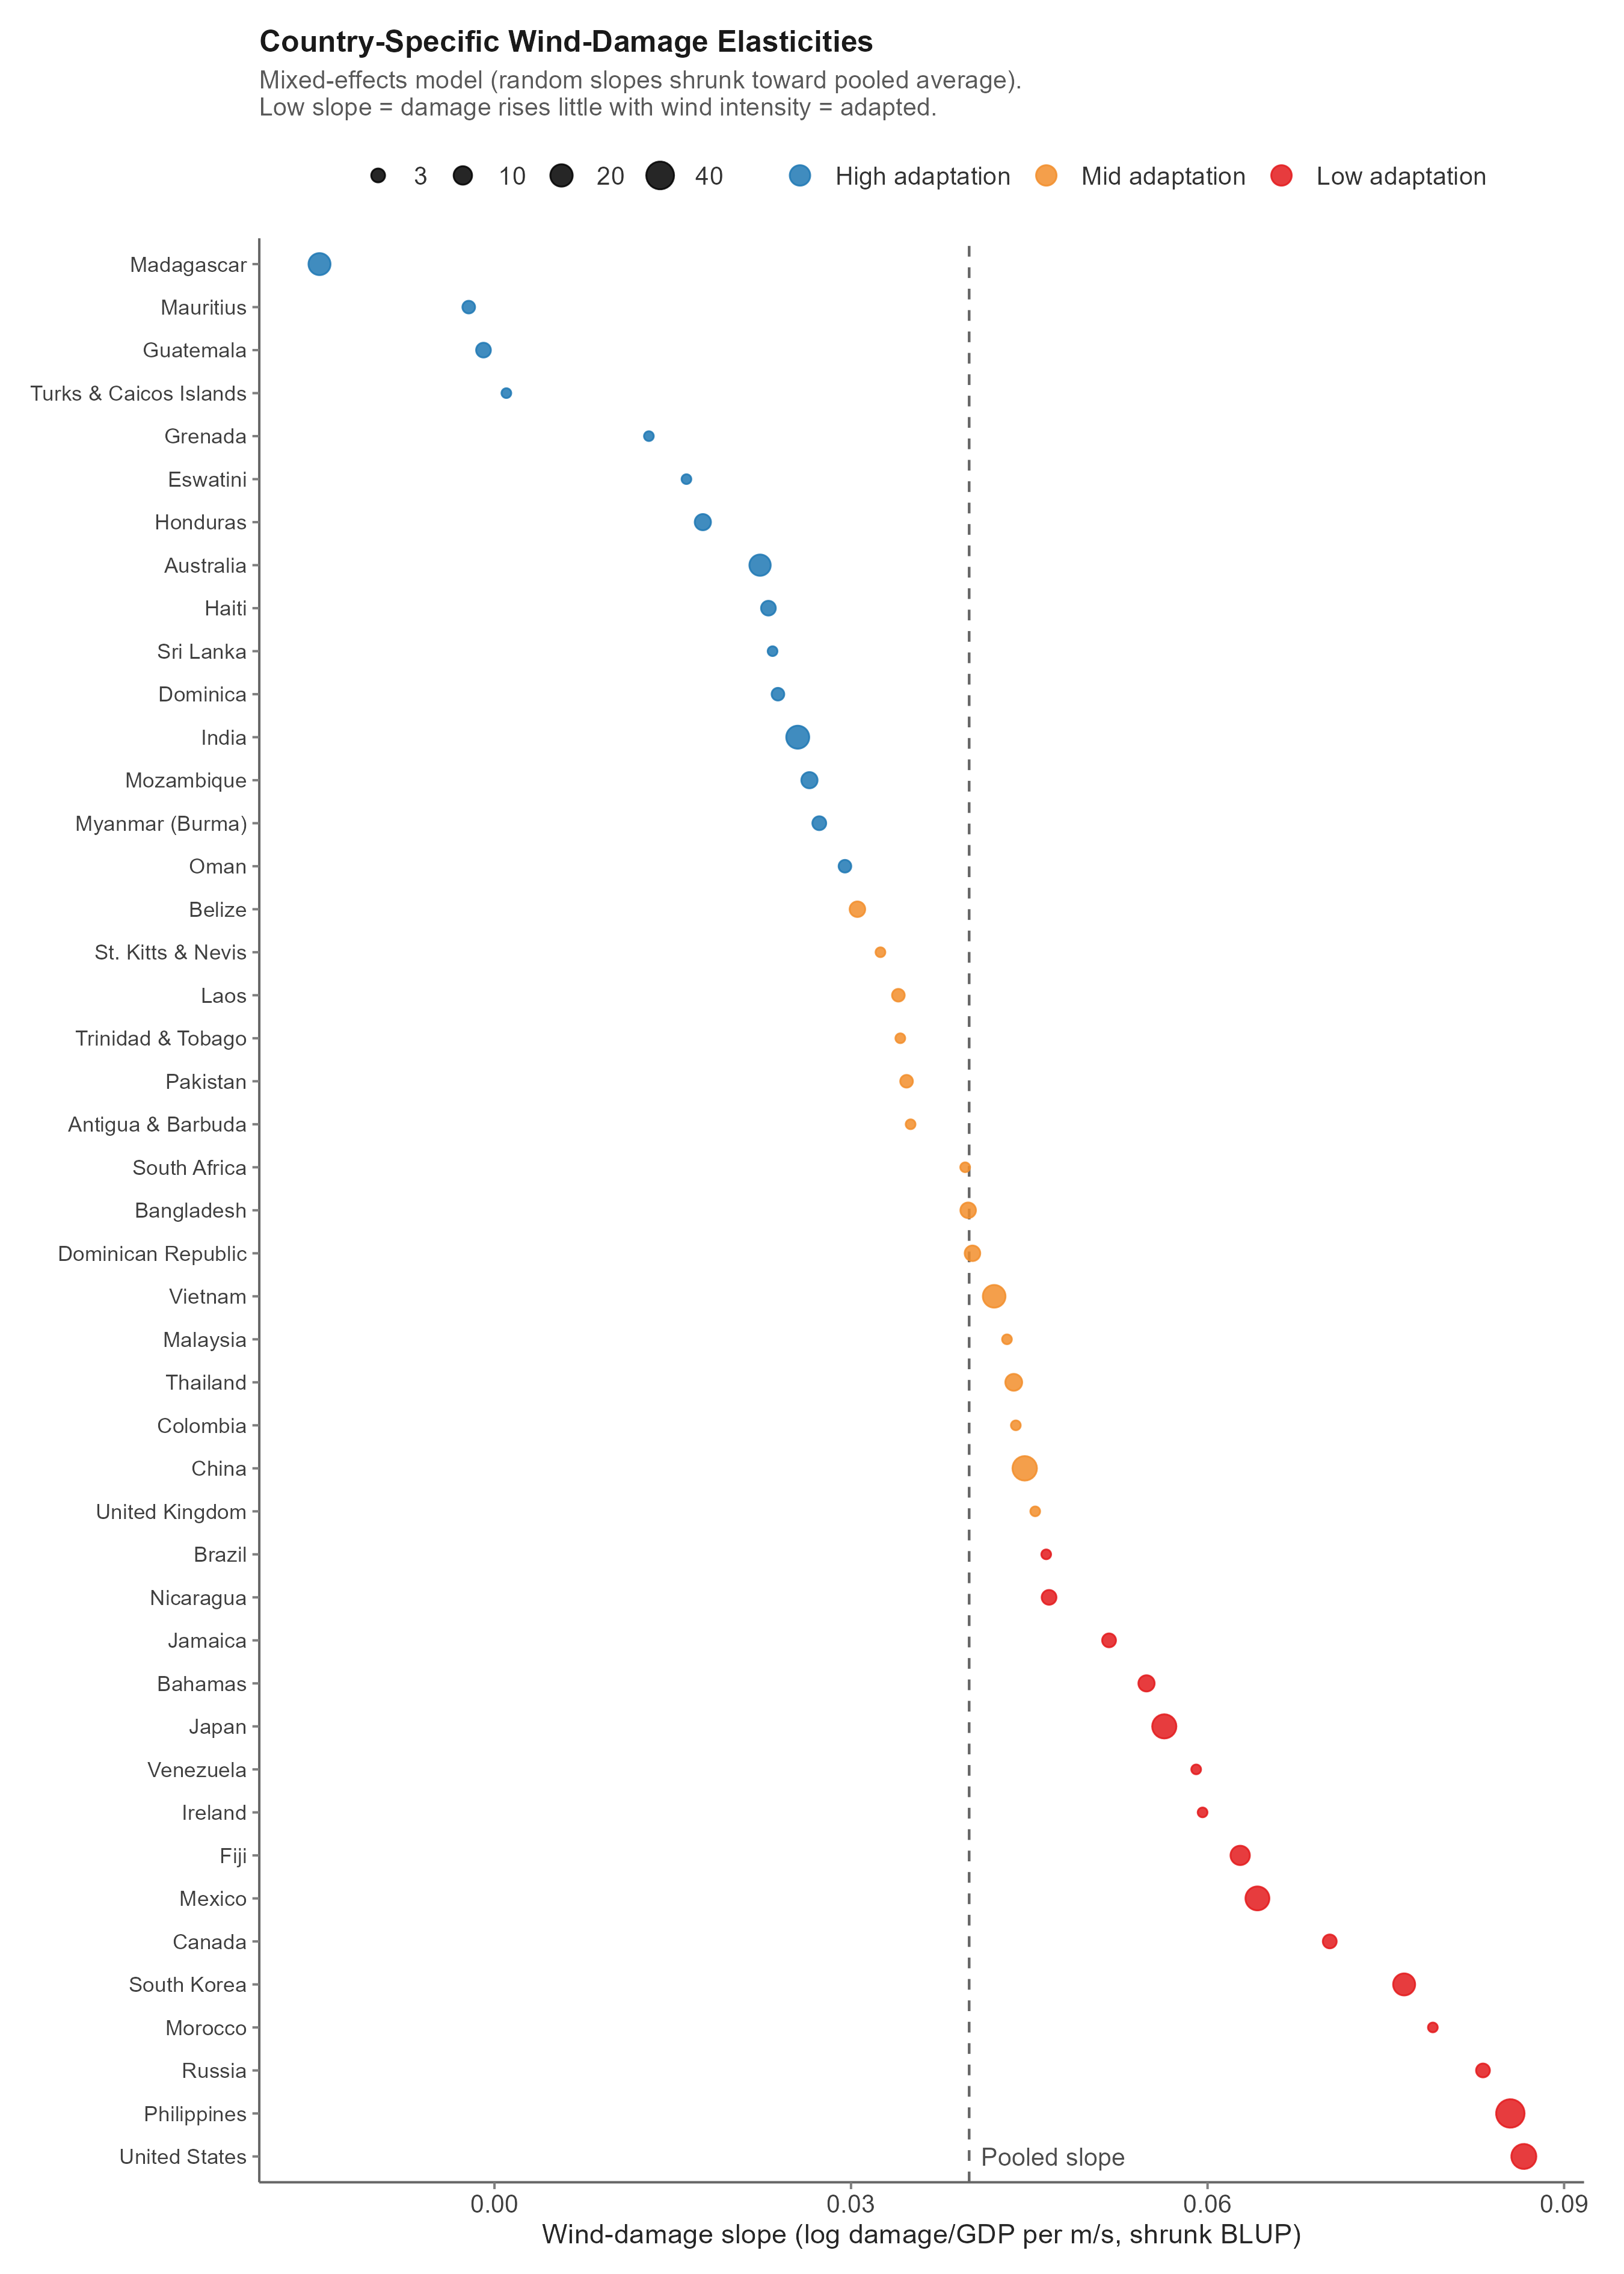
\includegraphics[width=0.88\textwidth,height=0.76\textheight,keepaspectratio]{figures/adapt_rank.png}

\smallskip\small
Shrunk BLUP slopes from the mixed-effects model.
Dashed line = pooled slope.
Countries with few damage observations are pulled toward the pooled average.
\end{frame}

\begin{frame}{Adapted Countries Recover Faster}
\centering
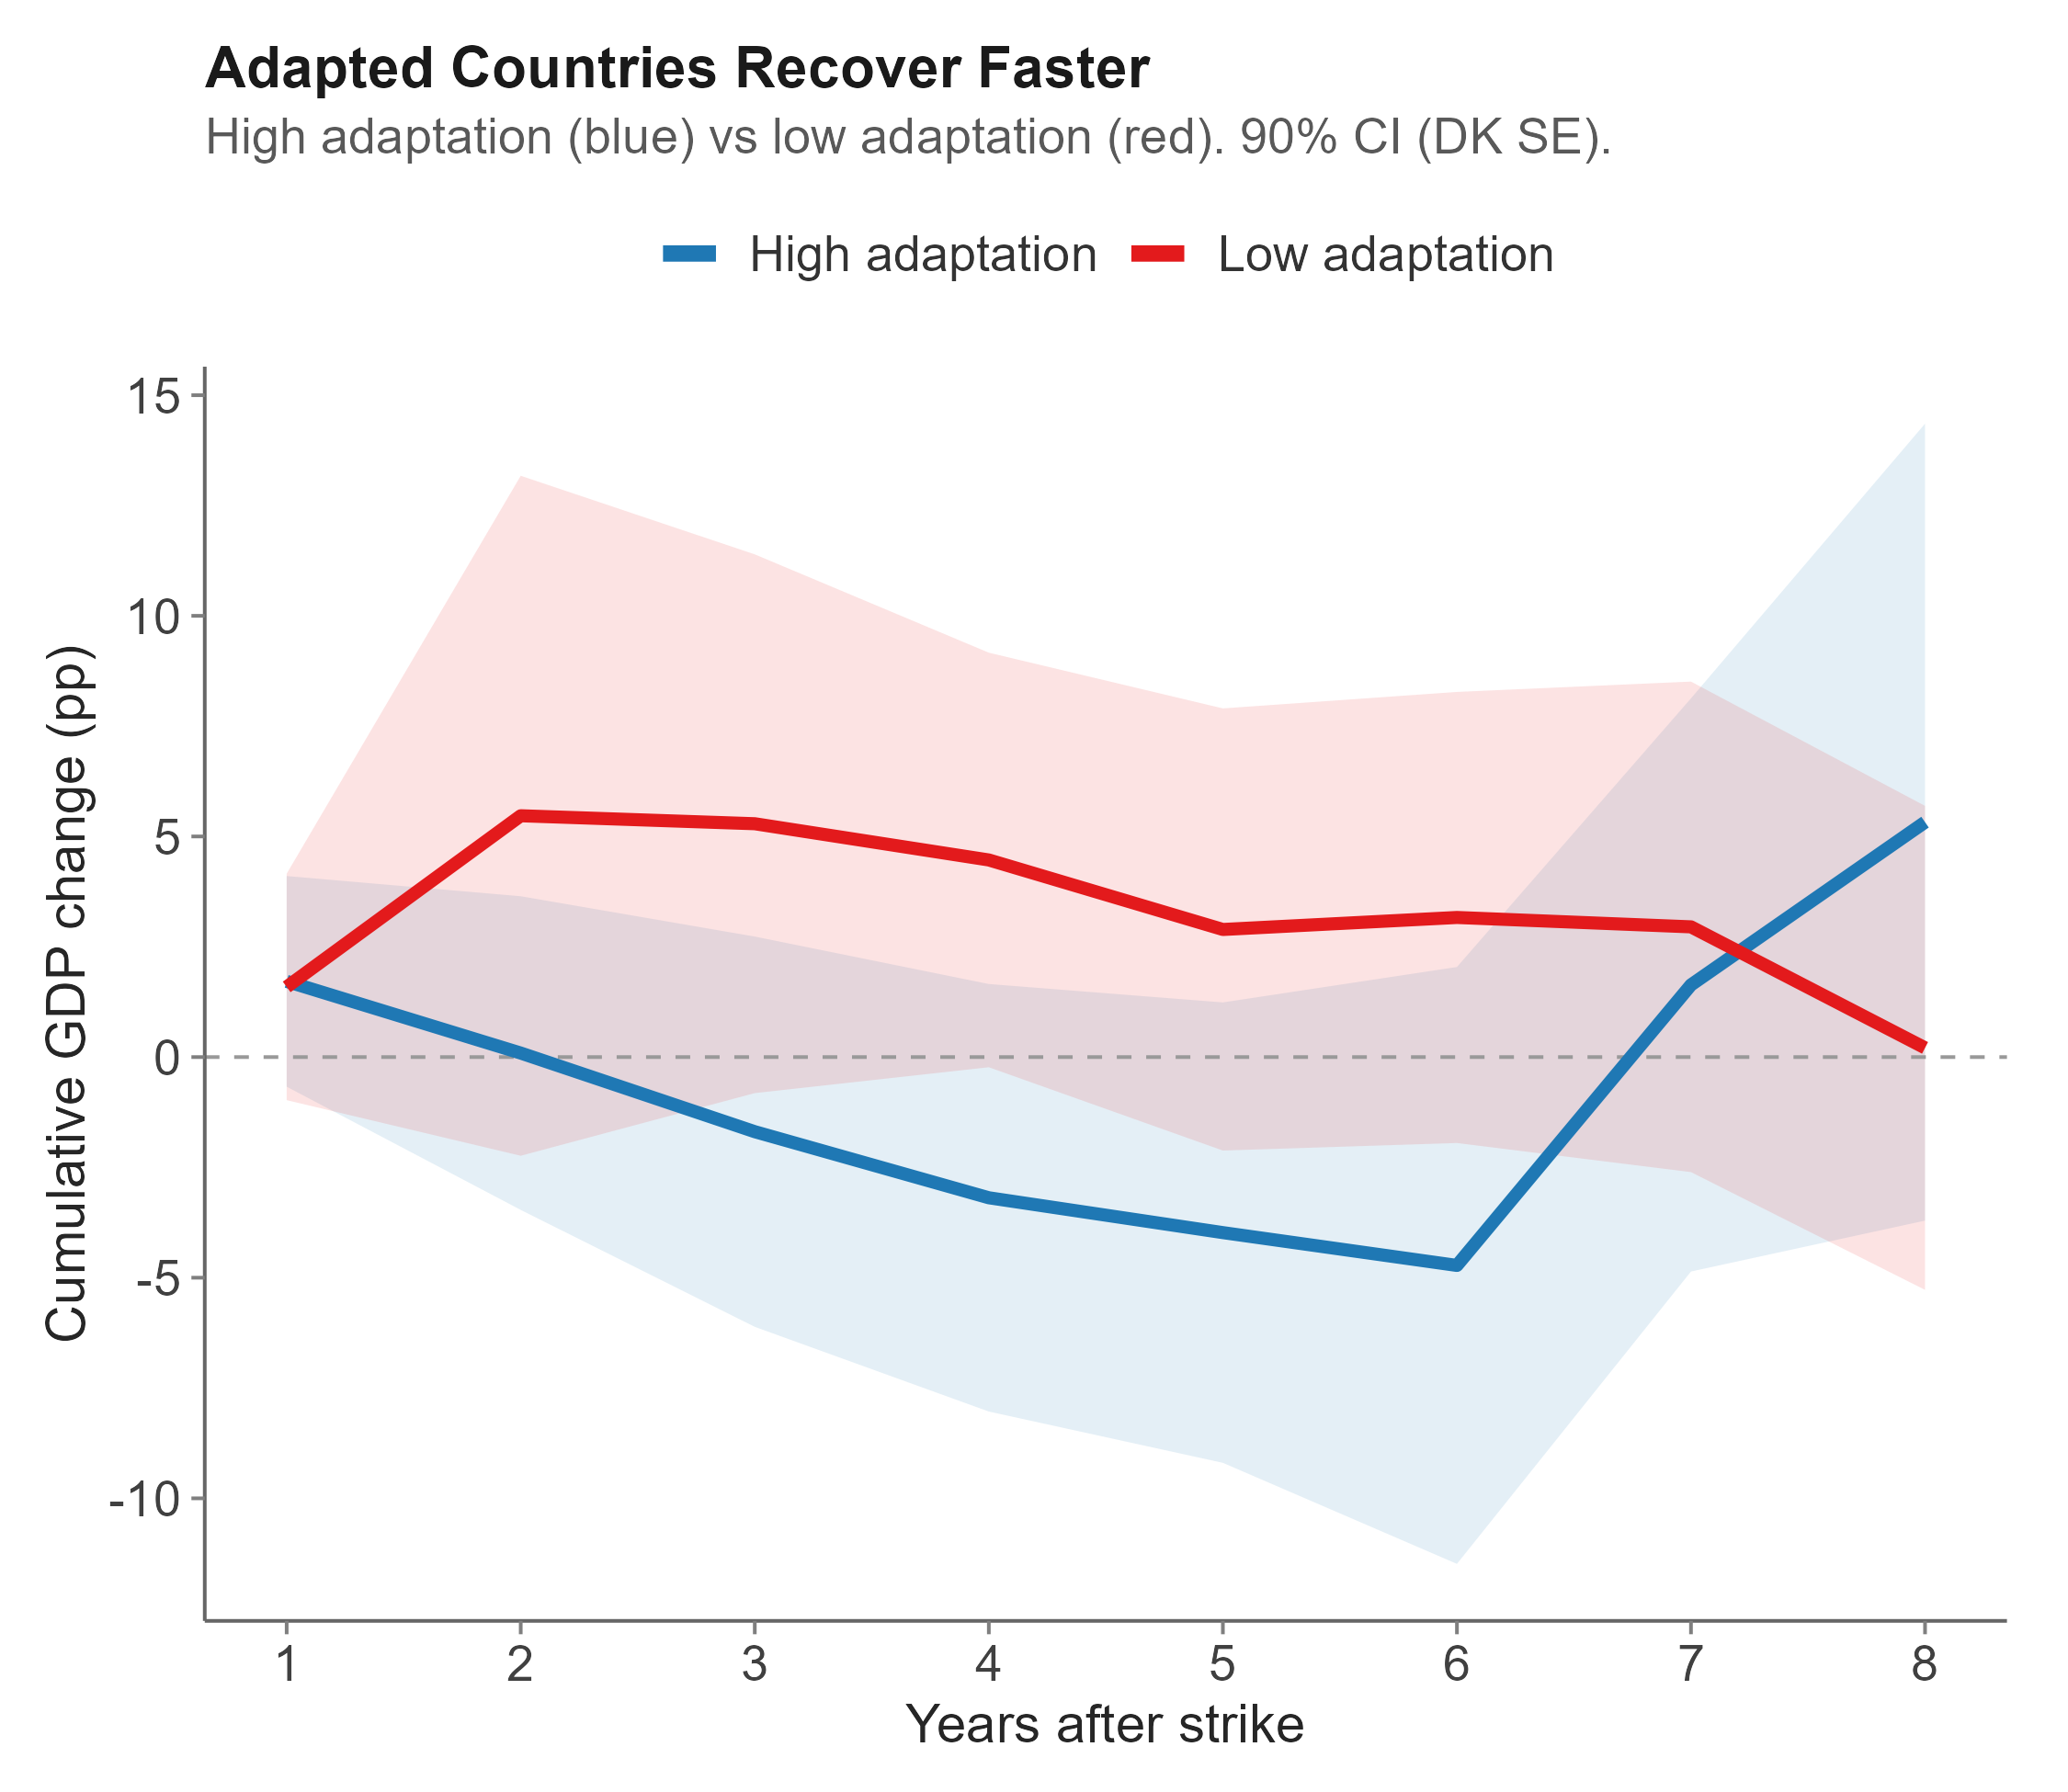
\includegraphics[width=0.80\textwidth,height=0.72\textheight,keepaspectratio]{figures/irf_by_adaptation_hl.png}

\smallskip\small
LP IRF to a Cat\,1+ strike by adaptation tercile
(high adaptation in blue, low in red; 90\,\% CI, DK SE).
Countries with a flat damage-wind slope show a smaller and shorter-lived
GDP dip after a cyclone.
\end{frame}

\begin{frame}{All Three Terciles}
\centering
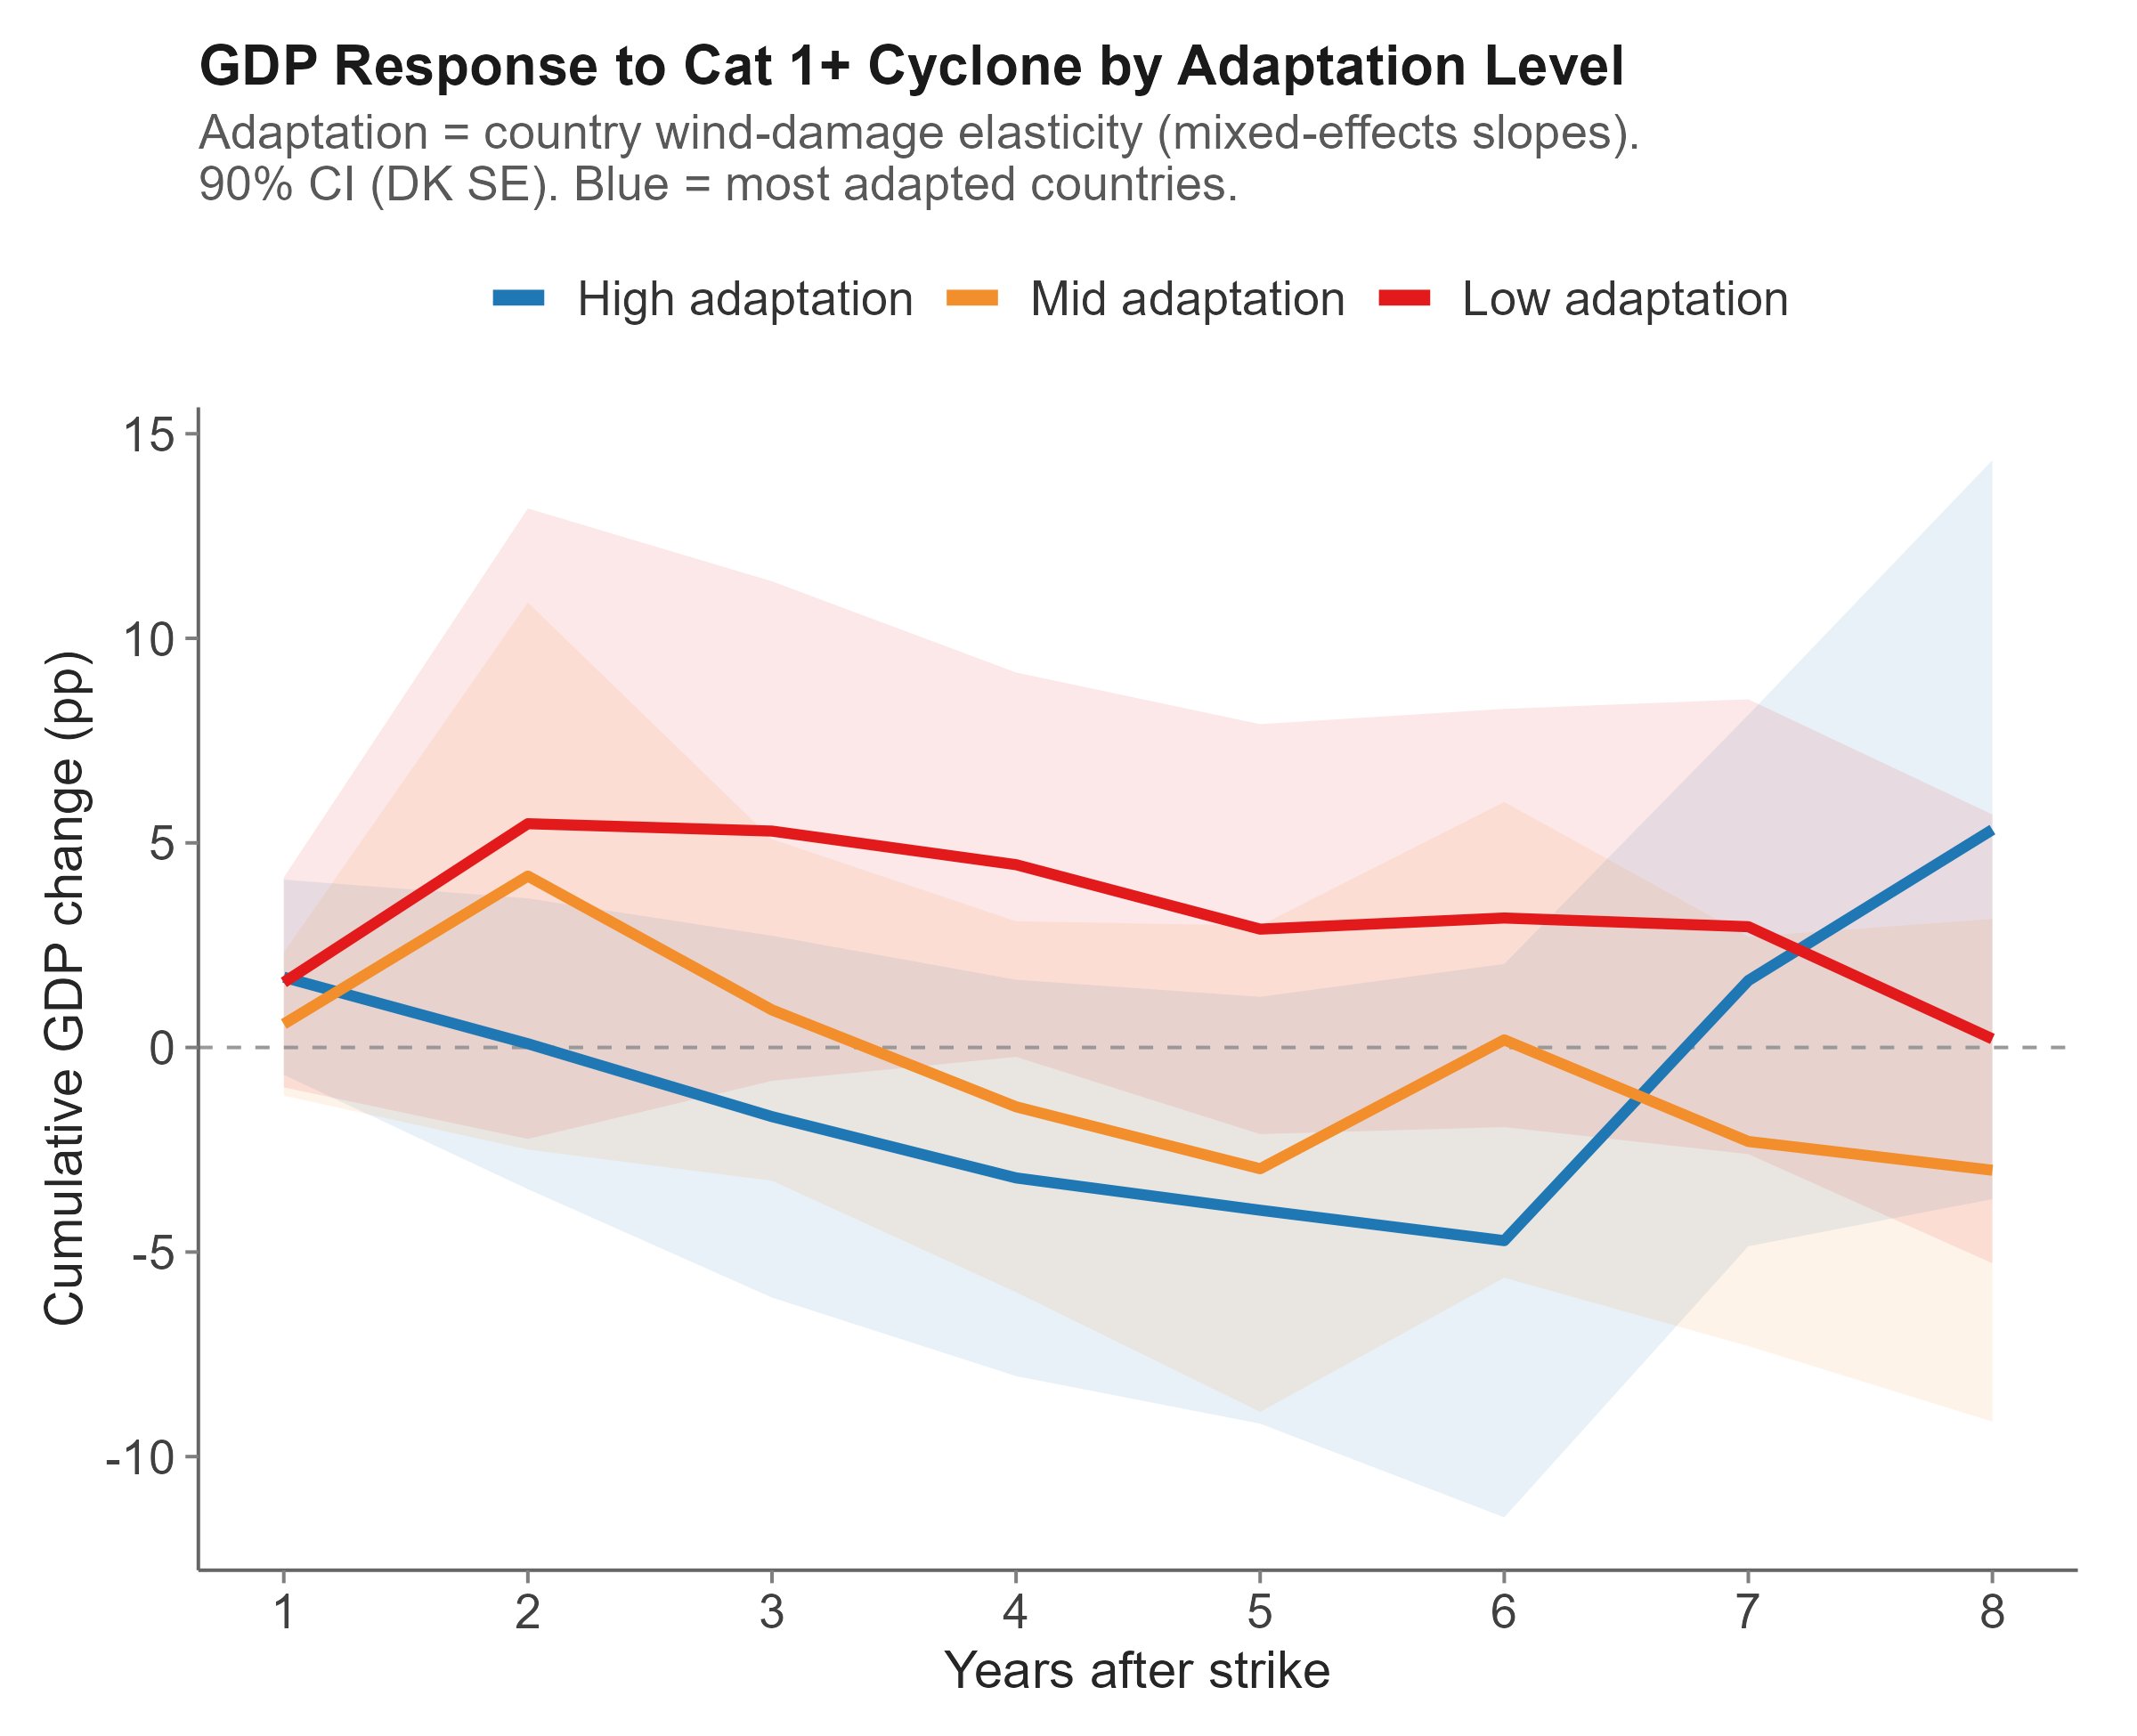
\includegraphics[width=0.80\textwidth,height=0.72\textheight,keepaspectratio]{figures/irf_by_adaptation.png}

\smallskip\small
Same LP IRF for all three adaptation terciles.
The gradient from high (blue) to low (red) adaptation is monotone:
less adapted countries suffer larger and more persistent GDP losses.
\end{frame}

\begin{frame}{Damage vs Wind by Adaptation Tercile}
\centering
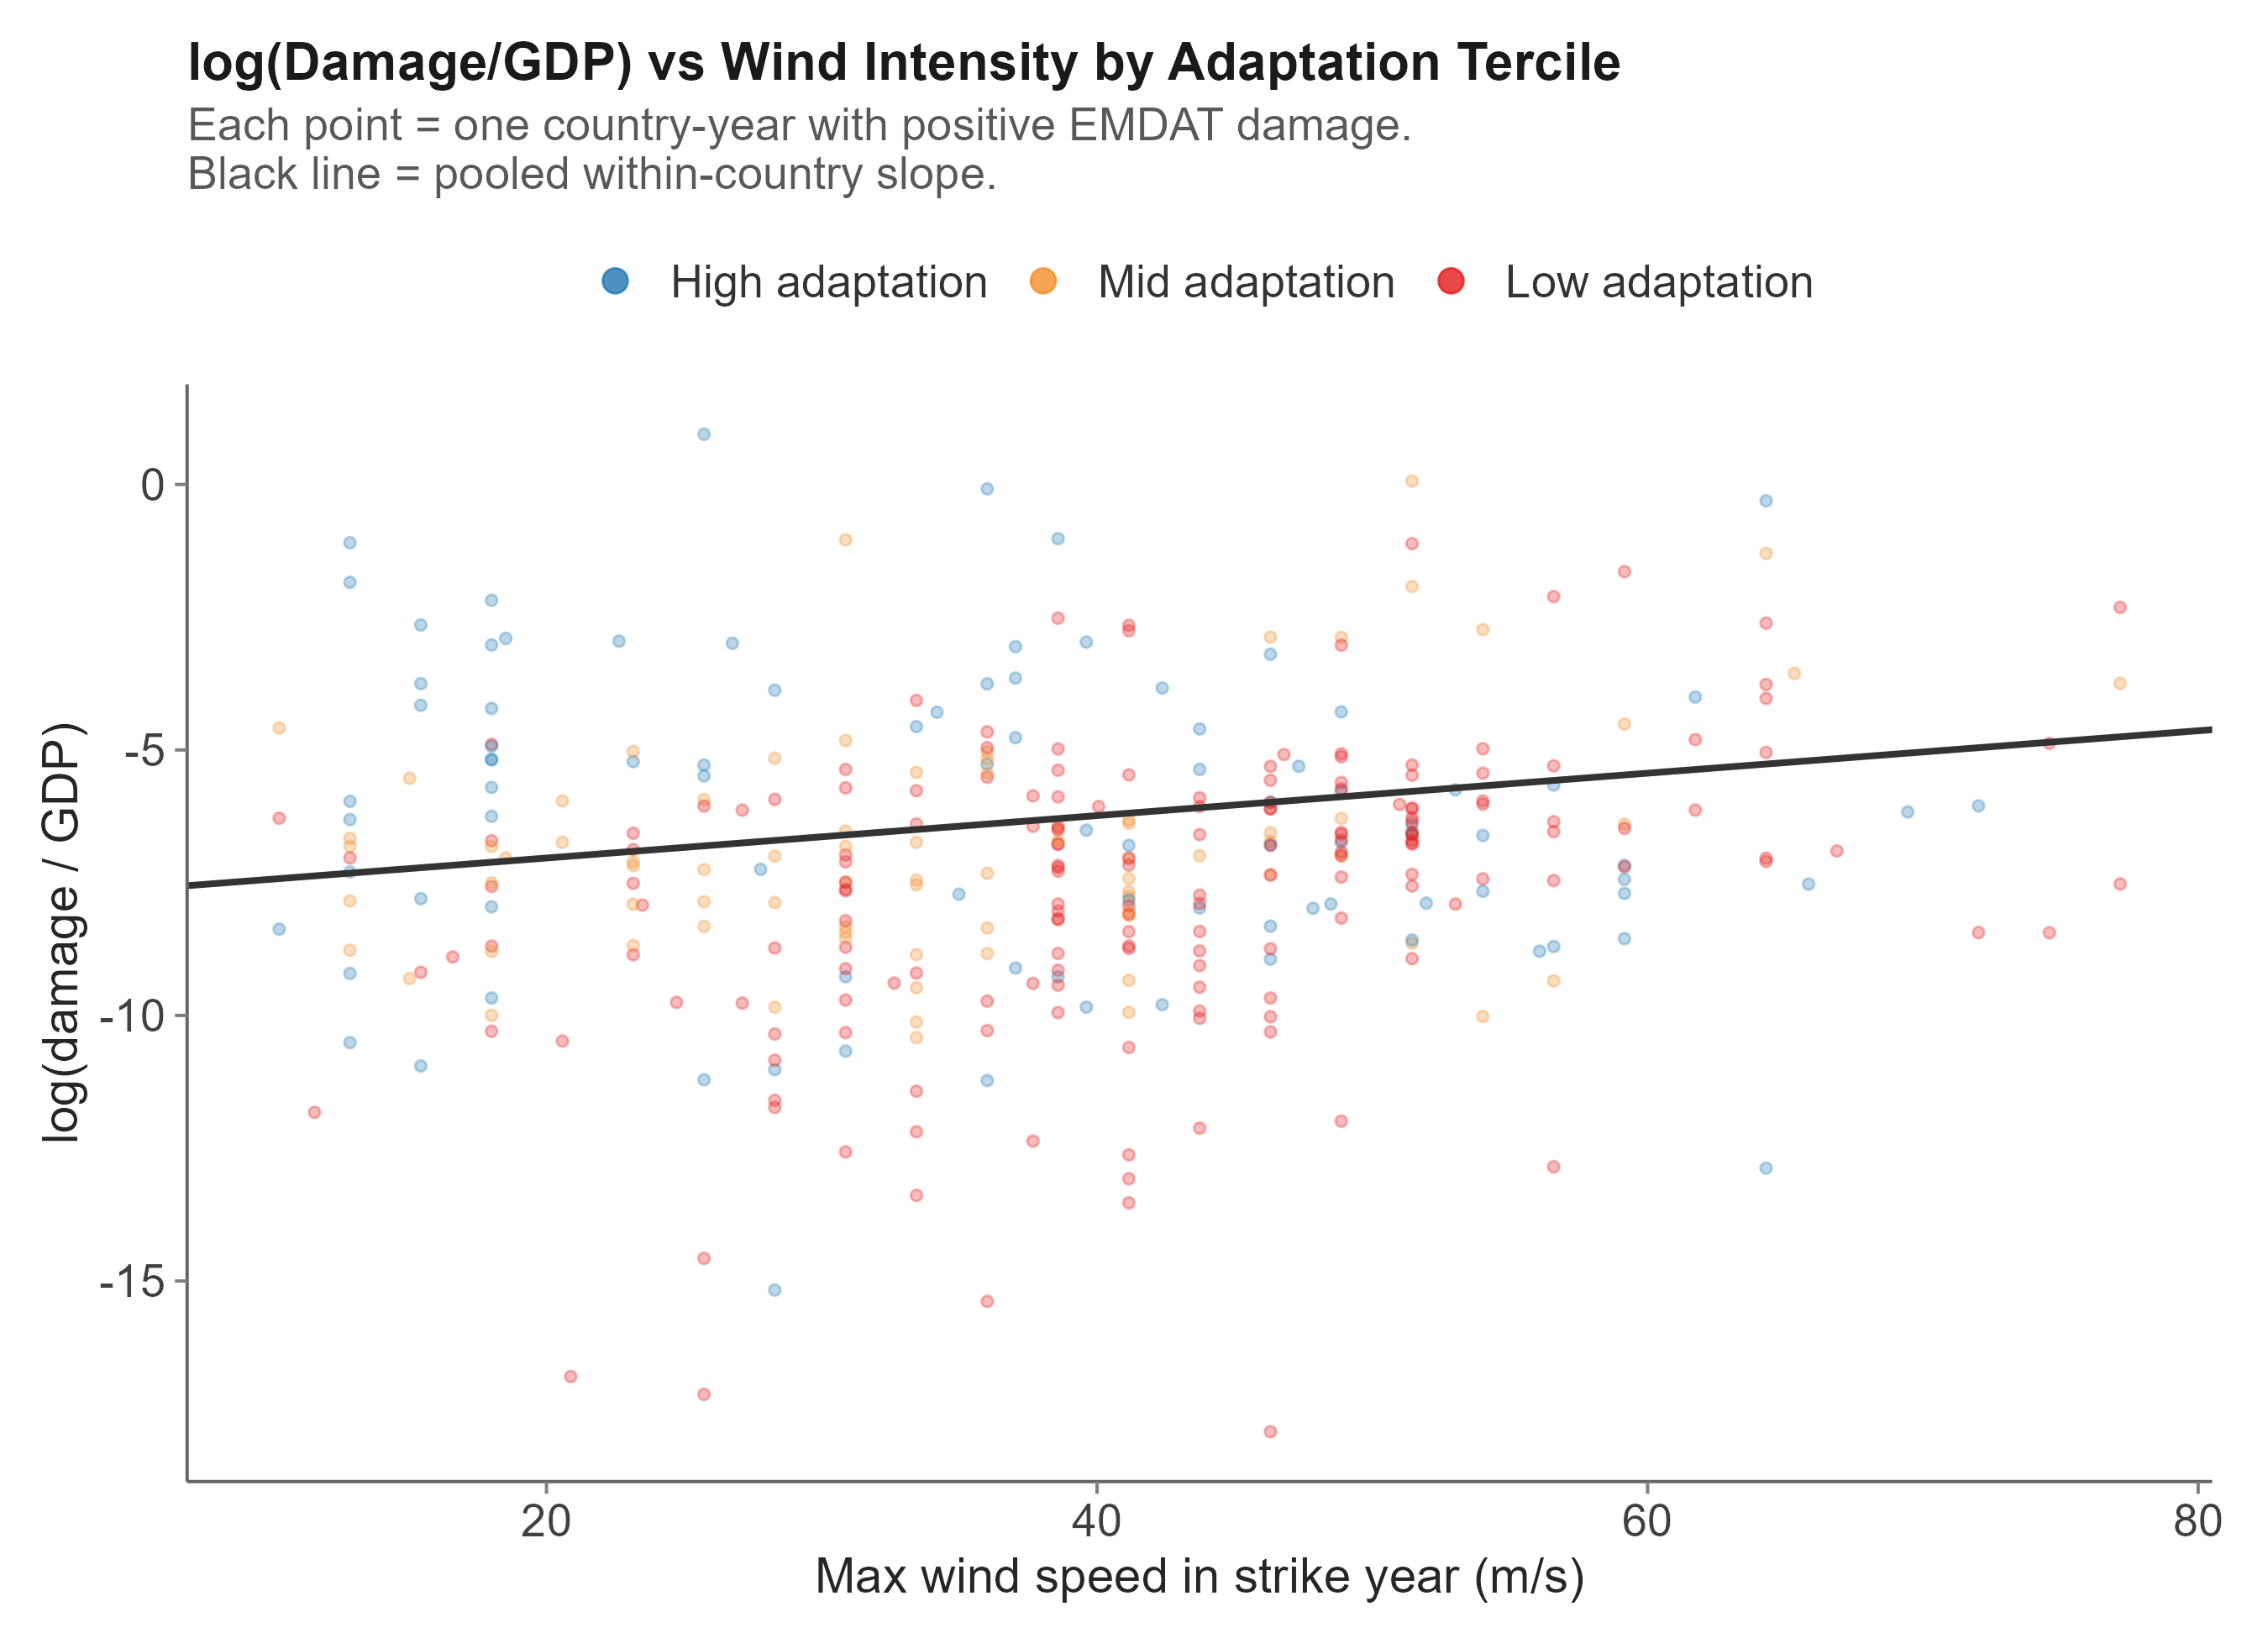
\includegraphics[width=0.82\textwidth,height=0.72\textheight,keepaspectratio]{figures/adapt_scatter.png}

\smallskip\small
Each point = one country-year with positive EMDAT damage.
Colour = adaptation tercile from the mixed-effects model.
Black line = pooled within-country slope.
\end{frame}

\end{document}
